%\documentclass[10pt,preprint]{aastex}  % for e-submission to ApJ
%\documentclass[12pt,preprint2]{aastex}  % for e-submission to ApJ - two column
\documentclass[onecolumn,iop]{emulateapj}  % this makes everything look like ApJ

\usepackage{graphicx, natbib, color, bm}

%%%% PUT NEW COMMANDS AND DEFINITIONS HERE %%%%
%%%% PUT NEW COMMANDS AND DEFINITIONS HERE %%%%

\newcommand{\Lmax}{\ell_{\rm max}}
\newcommand{\enzo}{{\small Enzo}}
\newcommand{\moray}{{\small Enzo+Moray}}
\newcommand{\zeus}{{\small ZEUS}}
\newcommand{\Lbox}{L_{\rm box}}
\newcommand{\Nroot}{N_{\rm root}}
\newcommand{\K}{\,\rm K}

%dcc color commands
\newcommand{\gtt}[1]{\textcolor{green}{{\tt#1}}}
\newcommand{\red}[1]{\textcolor{red}{#1}}
\newcommand{\blue}[1]{\textcolor{blue}{#1}}
\newcommand{\dcc}[1]{\textcolor{blue}{{\emph{#1}}}}

%mqk commands
\newcommand{\mqk}[1]{\textcolor{red}{mqk: #1}}

%dcc misc defs.
\def\grid{{\tt grid}}

\def\etal{{\sl et al.}}
\def\kms{{\rm km/s}}
\def\Ms{{\rm M_\odot}}
\def\nd#1{n_{ \rm #1}}
\def\k#1 {k_{{\rm #1}}}
\def\HH{H$_2$}
\def\HHp{H$_2^+$}
\def\Hp{H$^+$}
\def\Hm{H$^-$}
\def\Hep{He$^+$}
\def\Hepp{He$^{++}$}
\def\Dp{D$^+$}
\def\mHH{H_2}
\def\mH2p{H_2^+}
\def\mHp{H^+}
\def\mHm{H^-}
\def\mHep{He^+}
\def\mHepp{He^{++}}

%GB commands (overview section):
\newcommand{\myvec}[1]{\mathbf{#1}}
%\newcommand{\myvec}[1]{\vec{#1}}  %uncomment for traditional vectors
\newcommand{\rhop}{\rho^\prime}
\newcommand{\vecvp}{\myvec{v}^\prime}
\newcommand{\vecv}{\myvec{v}}
\newcommand{\vecB}{\myvec{B}}
\newcommand{\vecx}{\myvec{x}}
\newcommand{\Ep}{E^\prime}
\newcommand{\ep}{e^\prime}
\newcommand{\phip}{\phi^\prime}
\newcommand{\pp}{p^\prime}
\newcommand{\vecr}{\myvec{r}}
\newcommand{\rhob}{\rho}
\newcommand{\vecvb}{\vecv}
\newcommand{\Mach}{\mathcal{M}}
\newcommand{\fcond}{\myvec{F}_{\rm cond}}
\newcommand{\minmod}[2]{{\rm minmod} \left({#1},{#2} \right) }

%JHW commands
\newcommand{\cubecm}{\ifmmode{{\rm cm^{-3}}}\else{cm$^{-3}$}\fi}
\newcommand\unit[1]{\; \textrm{#1}}
\newcommand{\mh}{m_{\rm H}}



%%%%%%%%%%%%%%%%%%%%%%%%%%%%%%%%%%%%%%%%%%%%%

% Paper Outline  (last updated May 17, 2013)
%
% 1.  Introduction
% 2.  Physical equations and overview of numerical methodology
%   2.1 Physical equations
%   2.2 Overview of numerical methods
% 3.  The structured AMR method
% 4.  Fluid methods
%   4.1 PPM
%   4.2 MUSCL
%   4.3 MHD-CT
%   4.4 ZEUS 
% 5.  Gravity and N-body
%   5.1 Gravity
%   5.2 N-body dynamics
% 6. Microphysics
%   6.1  Chemistry
%   6.2  Radiative Cooling and heating
% 7. Radiation
%   7.1 Radiation: Homogeneous
%   7.2 Radiation: ray-tracing
%   7.3 Radiation: FLD
% 8. Other physics
%   8.1 Thermal conduction
%   8.2 Star formation & Feedback
% 9. Timestepping
% 10.  Analysis
% 11. Code tests
%   11.1 Verifying and Validating the Enzo code
%   11.2 Representative test problems
% 12. Parallelism 
%   12.1 Parallel strategy 
%   12.2 Parallel performance 
% 13. Code development methodology
% 14. Conclusions
%
%%%%%%%%%%%%%%%%%%%%%%%%%%%%%%%%%%%%%%%%%%%%%

\citestyle{aa}  % correct formatting for ApJ style files

\begin{document}

\title{Enzo: An Adaptive Mesh Refinement Code for Astrophysics}
\author{The Enzo Collaboration:}
\author{author 1}
\author{author 2}
\author{author 3...}

%\altaffiltext{1}{ Department of Astronomy, Columbia University,
%New York, NY, 10027, U.S.A.  Email: gbryan@astro.columbia.edu }
%\altaffiltext{2}{Center for Astrophysics and Space Sciences,
%University of California at San Diego.
%Email: mnorman,dcollins,akritsuk,jbordner@cosmos.ucsd.edu}
%\altaffiltext{3}{Theoretical Astrophysics (T-6), Los Alamos National
%Laboratories.  Email:  bwoshea@lanl.gov}
%\altaffiltext{4}{San Diego Supercomputing Center, University of California
%at San Diego.  Email: harkness@sdsc.edu}
%\altaffiltext{5}{Kavli Institute for Particle Astrophysics and Cosmology,
% Stanford University.  Email:  tabel@stanford.edu}

\begin{abstract}
This paper describes the open-source code \enzo, which uses a
block-structured adaptive mesh refinement to provide high spatial and
temporal resolution for modeling astrophysical fluid flows.  The code
is Cartesian and can be run in 1, 2, and 3 dimensions, and supports a
large variety of physics, including hydrodynamics, ideal and non-ideal
magnetohydrodynamics, N-body dynamics (and, more broadly, self-gravity
of fluids and particles), primordial gas chemistry, optically-thin
radiative cooling of primordial and metal-enriched plasmas, radiation
transport, and cosmological expansion.  In addition to explaining the
algorithms implemented, we present solutions for a wide range of test
problems, demonstrate the code's parallel scaling properties, and
discuss the \enzo\ collaboration's code development methodology.
\end{abstract}

\keywords{methods: numerical --- hydrodynamics}

\maketitle

%% Section: introduction

\section{Introduction}\label{sec.intro}


Many phenomena in astrophysics and cosmology require a high spatial and temporal dynamical range, and there are a number of numerical techniques that have been used to model such problems.  At the current time, the most common is a gridless, fully Lagrangian method call Smoothed Particle Hydrodynamcs \citep[SPH;][]{Lucy77, SPH} which has been very successful -- particularly for those situations dominated by gravity, where systems evolve over large spatial and temporal dynamic ranges.  Its development, however, is still at a relatively early stage when compared to the effort put into Eulerian, grid-based hydrodynamic schemes \citep[e.g.,][]{laney-1998, toro-1997, Woodward84}. 

Therefore, we would like to make use of the expertise that has been invested in Eulerian solvers; unfortunately, as originally developed, none of these schemes provide an easy way to adaptively and dynamically increase the spatial and temporal resolution in small volumes, as required by, for example, gravitational instability.  We have instead adopted an idea first suggested by \citet{Berger89} in the Computational Fluid Dynamics (CFD) community, which has become known as Structured Adaptive Mesh Refinement (SAMR).  The principle is to adaptively add and modify additional, finer meshes (``patches'') over regions that require higher resolution.  Since each patch has a simple geometry (Cartesian, in our case) the hyperbolic fluid-dynamical equations can be solved on that patch with a well-developed `off-the-shelf' numerical method.  In addition, it is relatively straightforward to add other advanced physics (e.g. magnetohydrodynamics, radiation transport, chemistry, etc.). This paper is devoted to describing how we have implemented this idea for astrophysics, including the addition of comoving coordinates, self-gravity, radiative cooling, chemistry, heat conduction, collisionless fluids, MHD, radiation transport, star formation and a range of other physical effects.

There have been many other numerical methods described in the astronomical literature which contain elements of this idea, or have a similar aim.  For example, an N-body solver \citep{Villumsen89} used non-adaptive meshing to increase the resolution in pre-selected regions.  This static approach, applied to hydrodynamics, has been used extensively \citep[e.g.,][]{Ruffert94, Anninos94}.  Adding adaptivity is a more recent enhancement, and there are now a number of N-body codes that possess this feature, both with and without  hydrodynamics  \citep{Couchman91, Jessop94, Suisalu95, Splinter96, Gelato97, ART97, Truelove98, flash_method, MLAPM01,  Yahagi01, RAMSES, Quilis04, Ziegler05, Zhang06, Astrobear09, Pluto-amr, GAMER, Nyx}.  Of these, perhaps the most comparable and widely used are FLASH \citep{flash_method}, which uses grid blocks of fixed size, and RAMSES \citep{RAMSES} and ART \citep{ART97}, both of which refine individual cells.   It is also possible to deform the grid to obtain high resolution \citep[e.g.,][]{Gnedin95, Xu97, Pen98}, and more recently a few grid codes have adopted an unstructured approach based on a moving Voronoi mesh \citep{Arepo10, Tess11}.

\enzo\ is a structured adaptive mesh refinement (SAMR) code that was originally developed for cosmological hydrodynamics and has been used on a wide variety of problems.  It has been expanded as a general tool for astrophysical fluid dynamics and is intended to be efficient, accurate and easily expanded.  Although many of the components of the code have been described in previous publications \citep{1995CoPhC..89..149B, BryanThesis96, Bryan97a, Bryan97b, Norman99, BryanCompSci99, Bryan01, Oshea04, 2007arXiv0705.1556N}, there has been no systematic and complete description of the code.  In this paper we provide that description, filling in many gaps and showing the code's performance for a wide variety of test problems.

The \enzo\ code has been extensively used over the last two decades in a wide variety of problems, and more than 100 peer-reviewed papers have been published based on results obtained with the code.  The code has previously been used to study a wide range of astrophysical systems, including galaxy clusters \citep{Loken02}, the interstellar medium \citep{Slyz05}, the intergalactic medium \citep{Fang01}, cooling flows \citep{Li12}, turbulence \citep{Kritsuk04}, and the formation of the first stars \citep{ABN02}.

Finally, we note that the numerical simulation of astronomical phenomena now plays a key role, along with observations and analytic theory, in pushing forward our understanding of the cosmos \citep[e.g.,][]{DecadalSurvey01, DecadalSurvey10}.   But along with this role comes responsibility.  We believe that those developing simulation tools must fulfill two key obligations: the first is to make those tools available to the community as a whole, much in the way that astronomical data is now regularly made publicly available.  The second is document, test and refine those methods so that they can be critically evaluated and expanded by others.  This paper represents one part of our attempt to meet our obligations with respect to the \enzo\ code.

The structure of the code is as follows.  In Section~\ref{sec.overview}, we first provide a top-level overview of the code method and structure.  This is designed to give a first broad-brush picture of the equations we aim to solve and the methods used to solve them.  Next, in Sections~\ref{sec.amr} through~\ref{sec.num.analysis}, we describe the methods we use in detail, reserving some of the longer descriptions of particular components for the appendix in order not to interrupt the flow of the paper.  The \enzo\ testing framework and code tests are described in Section~\ref{sec.tests}.  The parallelism strategy and scaling results are described in Section~\ref{sec.parallel}.  Finally, we discuss the code's development methodology (which is as far as we know unique in the astrophysics community) in Section~\ref{sec.development}.



%% Section:  Overview


\section{Physical Equations and Overview of Numerical Methodology}
\label{sec.overview}

We begin this section by first writing down the complete set of
physical equations that be solved by \enzo, and then briefly describe
the numerical algorithms that we use to solve these equations.  This
section is intended to be an overview of the \enzo\ code's
capabilities: thus, we gather all of the equations solved into a
single place and provide a brief and high-level introduction to the
numerics of the code.  Detailed descriptions of the individual
components are then provided in Section~\ref{sec.methods}.

% ====================================================

\subsection{Physical Equations}
\label{sec.equations}

% ----------------------------------------------------------------------------------------

%\subsubsection{Magnetohydrodynamics and Gravity}

The Eulerian equations of ideal magnetohydrodynamics including gravity
in a coordinate systems comoving with the cosmological expansion are
given by:

\begin{eqnarray} 
\frac{\partial \rho}{\partial t} 
          + \frac{1}{a} \nabla \cdot (\rho \vecv) & = & 0
        \label{eq:mass} \\
%
\frac{\partial \rho \vecv}{\partial t}  
   + \frac{1}{a} \nabla \cdot \left(\rho \vecv \vecv + \myvec{I}p^* - \frac{\vecB \vecB}{a} \right) & = &
    - \frac{\dot{a}}{a} \rho \vecv - \frac{1}{a} \rho \nabla \phi
    %
%          + \frac{1}{a} ( \vecv \cdot \nabla ) \vecv
%    & = & - \frac{\dot{a}}{a} \vecv 
%          - \frac{1}{a \rho} \nabla p
%          - \frac{1}{a \rho} (\nalba \times \vecB) \times \vecB
%          - \frac{1}{a} \nabla \phi, 
        \label{eq:momentum} \\
%
\frac{\partial E}{\partial t} 
+ \frac{1}{a} \nabla \cdot \left[ (E + p^*) \vecv -  \frac{1}{a} \vecB (\vecB \cdot \vecv) \right] & = &
     - \frac{\dot{a}}{a} \left( 2E - \frac{B^2}{2a} \right)  - \frac{1}{a} \vecv \cdot \nabla \phi 
     - \Lambda + \Gamma + \frac{1}{a^2} \nabla \cdot \fcond
     %
%         + \frac{1}{a} \vecv \cdot \nabla E
 %  & = & - \frac{\dot{a}}{a} (3 \frac{p}{\rho} + {\vecv \cdot \vecv} )
  %       - \frac{1}{a \rho } \nabla \cdot (p \vecv) 
%%\nonumber   & &   %uncomment for 2-column
 %        - \frac{1}{a} \vecv \cdot \nabla \phi 
 %               + \Gamma - \Lambda.
       \label{eq:total_energy}  \\
%
\frac{\partial \vecB}{\partial t} - \frac{1}{a}  \nabla \times (\vecv \times \vecB) & = & 0 \label{eq:induction}
\end{eqnarray}

%\begin{eqnarray} 
%\frac{\partial \rho}{\partial t} 
%          + \vecv \cdot \nabla \rho
%    & = & - \rho \nabla \cdot \vecv,
%        \label{eq:mass} \\
%%
%\frac{\partial \vecv }{ \partial t} 
%          + ( \vecv \cdot \nabla ) \vecv 
%    & = & - \frac{1}{\rho} \nabla p
%          - \nabla \phi,
%        \label{eq:momentum} \\
%%
% \frac{\partial E}{\partial t} + \vecv \cdot \nabla E
%    & = & - \frac{1}{\rho} \nabla \cdot (p \vecv) 
%          - \vecv \cdot \nabla \phi
%%\nonumber          \\  & &     % uncomment for 2-column
%     + \Gamma - \Lambda
%        \label{eq:total_energy}
%\end{eqnarray}
%
In these equations, $E$, $\rho$, $\vecv$, and $\vecB$ are the comoving
total fluid energy, comoving baryonic density, peculiar velocity, and
comoving magnetic field strength, respectively.  $\myvec{I}$ is the
identity matrix, and $a$ is the cosmological expansion parameter
(which is discussed in more detail below).
The first equation represents conservation of mass, the second, conservation of momentum, and the third, conservation of total fluid (kinetic plus thermal) energy.  They are respectively, the first, second and third moments of the Boltzmann equation.  The fourth equation is the magnetic induction equation.   Terms representing radiative cooling ($\Lambda$) and heating ($\Gamma$) enter on the right-hand side of the energy equation (\ref{eq:total_energy}), as well as the flux due to thermal heat conduction ($\fcond$).

The total fluid energy $E$ is given by:
\begin{equation}
E =  e + \frac{\rho v^2}{2}  + \frac{B^2}{2a}
        \label{eq:total_energy_def}.
\end{equation}
where $e$ is the comoving thermal energy density, and the total isotropic pressure $p^*$ is given by
\begin{equation}
p^* = p + \frac{B^2}{2a}
\end{equation}
The equations are closed with the equation of state and Poisson's equation (we work in the Newtonian limit):
%
\begin{eqnarray}
%
e   & = & p / [(\gamma - 1) \rho ],
        \label{eq:eq_of_state} \\
%
\nabla^2 \phi & = & 4 \pi G \rho_{\rm total}
%                   + 3 p_{total}/c^2) - \Lambda. 
        \label{eq:potential}
\end{eqnarray}
%
The equation of state is shown here for an ideal gas with a ratio of specific heats $\gamma$.
Equation (\ref{eq:potential}) includes contributions to the
gravitational potential $\phi$ from the total mass density $\rho_{\rm
  total}$.  Although we write the equations including both MHD and
comoving coordinates, the code can operate both in the pure
hydrodynamic limit ($\vecB = 0$) and without cosmological expansion
($a = 1$, $\dot{a} = 0$).

% ----------------------------------------------------------------------------------------

%\subsubsection{Comoving Coordinates}

For completeness, we note here that as part of the usual transformation to comoving coordinates, we have defined a set of comoving quantities.  See, for example, \citet{Peebles93} for more details.  Specifically, we define:
\begin{eqnarray}
\vecx & = & \vecr/a, \\
\vecv & = & a \hspace{0.5mm} d\vecx/dt = 
              \vecvp - \dot{a}\vecx, \\
\rho    & = & a^3 \rhop,   \\
p       & = & a^3 \pp, \\
E       & = & a^3 (\Ep - 
              \dot{a} \vecx \cdot \vecvp - 
              \frac{1}{2} \dot{a}^2 \vecx^2), \\
\phi    & = & \phip + \frac{1}{2} a \ddot{a} \vecx^2. \\
\vecB & = & a^2 \vecB^\prime
\end{eqnarray}
where primes indicate the usual quantities defined in a fixed frame frame, $\vecr$ is the proper distance and $\vecx$ is the comoving distance.

%These definitions result in the following comoving equivalents to eqs. 
%(\ref{eq:mass})-(\ref{eq:potential}).
%%
%
%\begin{eqnarray} 
%\frac{\partial \rhop}{\partial t} 
%          + \frac{1}{a} \vecvp \cdot \nabla \rhop 
%    & = & - \frac{1}{a} \rhop \nabla \cdot \vecvp, 
%        \label{eq:mass_prime} \\
%%
%\frac{\partial \vecvp}{\partial t}  
%          + \frac{1}{a} ( \vecvp \cdot \nabla ) \vecvp 
%    & = & - \frac{\dot{a}}{a} \vecvp 
%          - \frac{1}{a \rhop} \nabla \pp 
%          - \frac{1}{a} \nabla \phip, 
%        \label{eq:momentum_prime} \\
%%
%\frac{\partial \Ep}{\partial t} 
%         + \frac{1}{a} \vecvp \cdot \nabla \Ep 
%   & = & - \frac{\dot{a}}{a} (3 \frac{\pp}{\rhop} + {\vecvp \cdot \vecvp} )
%         - \frac{1}{a \rhop } \nabla \cdot (p \vecvp) 
%%\nonumber   & &   %uncomment for 2-column
%         - \frac{1}{a} \vecvp \cdot \nabla \phip 
%                + \Gamma - \Lambda.
%       \label{eq:total_energy_prime} \\
%%
%\Ep  & = & \ep + \frac{1}{2} {\vecvp \cdot \vecvp},
%        \label{eq:total_energy_def_prime} \\
%%
%\ep                  & = & 
%        \pp/\left[ \left( \gamma - 1 \right) \rhop \right],
%      \label{eq:state_prime} \\ 
%{\nabla}^2 \phip    & = & 
%        \frac{4\pi G}{a} ( \rhop_{total} - \rhop_0 ).
%      \label{eq:poisson}
%\end{eqnarray}
%%
%%We use the proper peculiar baryonic velocity $\vecv_b \equiv a(t) d\vecx / dt$, proper pressure $p$, and modified gravitational potential $ \phi $ which is related to the potential in proper coordinates $\Phi$ by 
%%$$\phi \equiv \Phi + \frac{1}{2} a \ddot{a} \vecx^2. $$
%%The density, however, is comoving:
%%$$\rho_b \equiv \rho_{b,proper}a(t)^3, $$
The expansion parameter $a \equiv 1/(1 + z)$ follows the expansion of a smooth, homogeneous background, where $z$, the redshift, is a function only of $t$.  All derivatives are determined with respect to the comoving position $\vecx$, which is defined simply to remove the universal expansion from the coordinate system.

The evolution of $a(t)$ is governed by the formula for the expansion of an isotropic, homogeneous universe:
%
\begin{eqnarray}
\frac{\ddot{a}}{a} & = & 
      - \frac{4 \pi G }{3 a^3 } (\rho_0 
      + 3p_0/c^2) 
      + \Lambda_c /3 .
      \label{eq:expansion} 
\end{eqnarray}
%
Here, $\rho_0$ is the mean comoving mass density (including both baryonic and dark matter), $p_0$ is the comoving background pressure contribution, and $\Lambda_c$ is the cosmological constant.
%$\gamma$ is the ratio of specific heats, and $\Lambda$ is the cosmological constant.
%We note that if $\gamma$ is not $5/3$ then $E$ in the first term on
%the right side of eq.~(ref{eq:total_energy}) must be replaced with 
%eq.~(\ref{eq:state}).
This system of equations is limited to the non-relativistic regime and assumes that curvature effects are not important --- both assumptions are reasonable as long as the  size of the simulated region is small compared to the radius of curvature and the Hubble length $c/H$ ($c$ is the speed of light and $H$ is the Hubble constant).

It is clear that the evolution equations are equivalent to the fixed coordinate version in the limit in which $a = 1$ and $\dot{a} = 0$.  We include the cosmological terms with the understanding that we are not restricting ourselves to cosmological applications.

%\subsubsection{Particles}

Any collisionless component (e.g. dark matter, stars) is modeled by particles which are governed by Newton's equations in comoving coordinates:
%
\begin{eqnarray}
\frac{d \vecx}{dt} 
    & = & \frac{1}{a} \vecv, 
          \label{eq:dm_position} \\
\frac{d \vecv}{dt} 
    & = & - \frac{\dot{a}}{a} \vecv
          - \frac{1}{a} \nabla \phi, 
          \label{eq:dm_velocity} 
\end{eqnarray}
%
The particles also make a contribution to the potential through their contribution to Poisson's equation.

%\subsubsection{Chemistry}

In addition, we can solve the mass conservation equations for a set of chemical species and reactions.  For any species $i$ with comoving number density $n_i$, these equations have the form:
\begin{equation}
\frac{\partial n_i}{\partial t} 
          + \frac{1}{a} \nabla \cdot (n_i \vecv) = 
        k_{ij}(T) n_i n_j 
      + \Gamma^{ph}_j n_j 
        \label{eq:species_evolution}
\end{equation}
where $k_{ij}$ are the rate coefficients for the two-body reactions
and are usually functions of only the gas species (we will
specifically note the cases where we either include three-body
reactions or have density-dependent rates).  The $\Gamma^{ph}_j$ are
destruction/creation rates due to photoionizations and/or
photodissociations.  Currently the species we can follow include H,
H$^+$, He, He$^+$, He$^{++}$, and $e^-$, as well as additional options
that add H$^-$, H$_2$, H$_2^+$, and  HD, D, and D$^+$.

%\red{
%There is some debate over whether to put in the hydro equations without cosmology, in addition
%to the equations that are already here.  Would this
%be more or less clear?  We're leaning towards saying ``when cosmology is turned off,
% $\dot{a}$ goes to zero and $a$ goes to 1, and the poisson equation changes to blah blah blah'' 
%and assuming our readers can figure it out for themselves.
%We also want to emphasize that the heating and cooling is glossed over in this section, 
%and it's discussed more thoroughly later.
%} %end red
% GB: I agree this would be shorter, and maybe it is a better idea, but I think it's nice to be able
% GB: to include both equations and at the same time make the transformation to comoving coords
% GB: very clear -- this has engendered a lot of confusion in the past and one of the goals of writing
% GB this paper is to answer peoples questions before they ask them.


% GB: I commented out the following.  It has now been incorporated into the above discussion
% GB: (see my comments anove on why I think this is a good way to do it)
%
%\enzo\ solves the equations of ideal gas dynamics
%in a coordinate system that is comoving with the expanding universe:

%\begin{equation}
%\frac{\partial \rho_b}{\partial t} + \frac{1}{a} \vecv_b \cdot \nabla \rho_b =  \label{enzoconserve}
% - \frac{1}{a} \rho_b \nabla \cdot \vecv_b 
%\end{equation}

%\begin{equation}
%\frac{\partial \vecv_b}{\partial t} + \frac{1}{a} (\vecv_b \cdot \nabla) \vecv_b = \label{enzomomentum} 
%-\frac{\dot{a}}{a} \vecv_b - \frac{1}{a \rho_b} \nabla p - \frac{1}{a} \nabla \phi
%\end{equation}

%\begin{eqnarray}
%\frac{\partial E}{\partial t} + \frac{1}{a} \vecv_b \cdot \nabla E =  
%- \frac{\dot{a}}{a} \left( 3 \frac{p}{\rho_b} + \vecv_b^2 \right)  \nonumber \\
%- \frac{1}{a \rho_b} \nabla \cdot (p \vecv_b) \nonumber \\
%- \frac{1}{a} \vecv_b \cdot \nabla \phi + \Gamma - \Lambda
%\label{enzoenergy}
%\end{eqnarray}

%Where $\rho_b$ is the comoving baryon density, $\vecv_b$ is the baryon velocity, $p$ is the pressure, 
%$\phi$ is the modified gravitational potential (in comoving coordinates, which is related to
%the potential in proper coordinates $\Phi$ by $\phi \equiv \Phi + 0.5 $a\"{a}$ \vecx^2$) and 
%$a$ is the ``expansion parameter'' which describes the expansion of a smooth, homogeneous 
%universe as a function of time.  This expansion parameter is related to the redshift:  
%$a \equiv 1/(1+z)$.  All derivatives are in comoving coordinates.  $E$ is the specific
%energy of the gas (total energy per unit mass), and
%$\Gamma$ and $\Lambda$ represent radiative heating and cooling processes as described below.
%  Equations~\ref{enzoconserve}, \ref{enzomomentum}
%and \ref{enzoenergy} represent the conservation of mass, momentum and total (e.g.,
%kinetic plus thermal) fluid energy.

%The equations above are closed with three more equations:

%\begin{equation}
%E = p / [(\gamma - 1) \rho_b] + \vecv^2/2   \label{enzoeos}
%\end{equation}

%\begin{equation}
%\nabla^2 \phi = \frac{4 \pi G}{a} (\rho_b + \rho_{dm} - \rho_0 )
%\label{enzopoisson}
%\end{equation}

%\begin{equation}
%\frac{\ddot{a}}{a} = - \frac{4 \pi G}{3 a^3} (\rho_0 + 3 p_0 / c^2) + \Lambda/3.
%\label{enzocomove}
%\end{equation}

%where $\rho_{dm}$ is the comoving dark matter density, $\rho_0$ is the comoving
%background density 
%($\rho_0 \equiv \Omega_{matter} \rho_{crit}$) and $p_0$ is the background pressure, 
%$\gamma$ is the ratio of specific heats and $\Lambda$ is the cosmological constant.
%Equations~\ref{enzoeos}, \ref{enzopoisson} and~\ref{enzocomove} are the 
%equation of state, Poisson's equation in comoving form and an equation that 
%describes the evolution of the comoving coordinates (i.e. the formula for the 
%expansion of an isotropic, homogeneous universe). 
%All particles in the simulation are governed by Newton's equations in comoving 
%coordinates:

%\begin{equation}
%\frac{d \vecx_{part}}{dt} = \frac{1}{a} \vecv_{part}
%\label{enzopartvel}
%\end{equation}

%\begin{equation}
%\frac{d \vecv_{part}}{dt} = -\frac{\dot{a}}{a} \vecv_{part} - \frac{1}{a} \nabla \phi
%\label{enzopartmom}
%\end{equation}

%Where $\vecx_{part}$ and $\vecv_{part}$ refer to the position and peculiar velocity of any
%particles in the system.  Note that the system of equations~\ref{enzoconserve}-\ref{enzopartmom} 
%is valid only in regimes where relativistic effects are not
%important ($v_b, v_{dm} \ll c$, where c is the speed of light) 
%and where cosmological curvature effects are 
%unimportant, meaning that the simulation volume is much smaller than the radius
%of curvature of the universe, as defined as $r_{hub} \equiv c/H_0$, where $c$ is the
%speed of light and $H_0$ is the Hubble constant.

%\dcc{Fixed punctuation, added 'no mhd, rhd' caveat to Zeus statements.  This has caused
%confusion in the past.}

%\subsubsection{Magnetohydrodynamics}



%\subsubsection{Radiation transport: ray-tracing}

The code can include either a homogeneous radiation background (with possible local self-shielding corrections), or evolve an inhomogeneous radiation field either by directly solving the radiative transfer equation along rays or by solving a set of moment equations derived from the radiative transfer equation.  

The radiative transfer equation in comoving coordinates 
\citep[e.g.,][]{Gnedin97} reads
%
\begin{equation}
  \label{eq:rteqn}
  \frac{1}{c} \; \frac{\partial I_\nu}{\partial t} + 
  \frac{\hat{n} \cdot \nabla I_\nu}{\bar{a}} -
  \frac{H}{c} \; \left( \nu \frac{\partial I_\nu}{\partial \nu} -
  3 I_\nu \right) = -\kappa_\nu I_\nu + j_\nu .
\end{equation}
%
Here $I_\nu \equiv I(\nu, \mathbf{x}, \Omega, t)$ is the radiation
specific intensity in units of energy per time $t$ per solid angle per
unit area per frequency $\nu$.  $H = \dot{a}/a$ is the Hubble
constant, where $a$ is the scale factor.  $\bar{a} = a/a_{em}$ is the
ratio of scale factors at the current time and time of emission.  The
second term represents the propagation of radiation, where the factor
$1/\bar{a}$ accounts for cosmic expansion.  The third term describes
both the cosmological redshift and dilution of radiation.  On the
right hand side, the first term considers the absorption coefficient
$\kappa_\nu \equiv \kappa_\nu(\mathbf{x},\nu,t)$, and the second term
$j_\nu \equiv j_\nu(\mathbf{x},\nu,t)$ is the emission coefficient
that includes any point sources of radiation or diffuse radiation.

%\subsubsection{Radiation transport: moment method}

In the other limit, we solve an equation derived from integrating
the equation of radiative transfer over angles.  In particular, we use a
flux-limited diffusion approximation for cosmological radiative
transfer, with couplings to both the gas energy and chemical number
densities. The equations solved are:
\begin{eqnarray}
  \label{eq:fld_radiation}
  \frac{\partial E_r}{\partial t} + \frac1a \nabla\cdot\left(E_r \vecv \right) &=& 
    \nabla\cdot\left(D\nabla E_r\right) -
    \frac{\dot{a}}{a} E_r - c\kappa E_r + \eta, \\
  \label{eq:fld_heating}
  \frac{\partial e_c}{\partial t} &=& -\frac{2\dot{a}}{a} e_c + \Gamma - \Lambda,
%  \label{eq:fld_chemistry}
%  \partial_t {\mathrm n}_i + 
%    \frac1a \nabla\cdot\left({\mathrm n}_i \vec{v}_b\right) &=& 
%    \alpha_{i,j} {\mathrm n}_e {\mathrm n}_j - {\mathrm n}_i
%    \Gamma_i^{ph}, \quad i=1,\ldots,N_s,
\end{eqnarray}
where $E_r$ is a grey radiation energy density and $e_c$ is the
internal energy correction due to photo-heating and chemical cooling.
%and ${\mathrm n}_i$ correspond to the chemical number densities of
%HI, HII, HeI, HeII and HeIII, and ${\mathrm n}_e$ is the electron
%number density.  
Here, we define the grey radiation energy density
through first assuming a fixed frequency spectrum, i.e.
$E_{\nu}(\nu,\vec{x},t) = \tilde{E}_r(\vec{x},t) \chi(\nu)$, and then
defining the integrated quantity
\begin{equation}
\label{eq:grey_radiation_energy}
   E_r(\vec{x},t) \equiv \int_{\nu_0}^{\infty}
   E_{\nu}(\nu,\vec{x},t)\,\mathrm d\nu \  = \ 
   \tilde{E}_r(\vec{x},t) \int_{\nu_0}^{\infty} \chi(\nu)\,\mathrm d\nu.
\end{equation}
In addition, $D$ in (\ref{eq:fld_radiation}) is the {\em Larsen
square-root flux-limiter} \citep[see][]{Morel2000}, $\kappa$ is the total
opacity, $\eta$ is the field of radiation sources, $\Gamma$ provides the
radiation induced photo-heating, and $\Lambda$ the chemical
cooling.
%, $\alpha_{i,j}$ are the reaction rate coefficients defining
%the interactions between species ${\mathrm n}_i$ and ${\mathrm n}_j$,
%and $\Gamma_i^{ph}$ are the radiation induced photo-ionization rates. 

%\subsubsection{Thermal conduction}

Enzo implements the equations of isotropic heat conduction in a manner
similar to that of \citet{2007ApJ...664..135P}, where we model the
flux of isotropic heat transport:

\begin{equation}
\fcond = -\kappa_{sp} \nabla T
\end{equation}

Where $\kappa_{sp}$ is the Spitzer conduction coefficient
\citep{1962pfig.book.....S} and T is the baryon temperature (with
fluids explicitly assumed to be single-temperature).  Saturation of the heat flux in
high-temperature, low-density regimes (such as the intracluster medium
in galaxy clusters) is taken into account.  Thermal conduction in a
plasma can be strongly affected by the presence of magnetic field
lines, which may strongly suppress heat flow perpendicular to the
magnetic field.  In that case, we allow for heat transport only along
the magnetic field lines in simulations that include this physics, as follows:

\begin{equation}
\fcond= -\kappa_{sp} \hat{\textbf{b}} (\hat{\textbf{b}} \cdot \nabla T)
\end{equation}

Where $\hat{\textbf{b}}$ is the unit vector denoting the direction of the
magnetic field.  In both the isotropic and anisotropic limits, we
assume that conductivity can be suppressed relative to the ideal
Spitzer conductivity, and express this as a multiplicative constant.

% ====================================================

\subsection{Overview of Numerical Methods}
\label{sec.method_overview}

In this section, we briefly describe the numerical methods which are
used to solve the equations outlined in Section~\ref{sec.equations}.  We
proceed through the numerical methods in the same order as will be used in
section~\ref{sec.methods} so that there is a one-to-one correspondence
between each of the following overviews and the complete description
provided in that section.  The goal here is to introduce the reader to
the basic principles of the methods without drowning in detail.

\subsubsection{Structured Adaptive Mesh Refinement}

The primary purpose of the \enzo\ code is its Adaptive Mesh Refinement (AMR)
capability, which allows it to reach extremely large dynamical ranges
with limited computational resources, opening doors previously closed
by finite memory and computational time. Unlike moving mesh methods
\citep{1995ApJS..100..269P,1995ApJS...97..231G} or  
methods that subdivide 
individual cells \citep{Adjerid}, Berger \& Collela's AMR (also referred 
to as \emph{structured} AMR) utilizes an adaptive hierarchy of grid 
patches at varying levels of resolution.  Each rectangular grid patch 
(referred to as a ``grid'') covers some region of space in its 
\emph{parent grid} which requires higher resolution, and can itself 
become the parent grid to an even more highly resolved \emph{child grid}. 

The grid hierarchy begins with the root grid, which covers the entire
domain of interest with a coarse, uniform, Cartesian grid. Then, as
the solution evolves and interesting regions form, finer meshes are
placed below these regions (we use the notation `below' to refer to
finer grids and `above' for coarser grids).  We restrict the ratio
between cell sizes to be an integer, typically 2 or 4, and refer to a
level as all grids with the same cell size.  In order to keep
things as simple as possible, the edges of subgrids must coincide with
the cell edge of its immediate parent (coarser) grid. Additionally,
the hierarchy can be initialized with one or more static grids if a
higher initial resolution is required.

Given the hierarchy at some time $t$, we advance the solution in the
manner of a W-cycle in a multigrid solver.  First, we determine the
maximum time step allowed for the coarsest grid based on a variety of
accuracy and stability criteria and advance the grid by that time
interval, $\Delta t_0$.  We then move down to the next level and
advance all the grids on that level by a timestep $\Delta t_1$
($\Delta t_1 \leq \Delta t_0$), which is the minimum of all the allowed
timesteps for those grids.  If there are more levels, we repeat this
procedure until the bottom level of the hierarchy has been reached.
Once there, we continue advancing the grids on the lowest level until
they have `caught up' to the next highest level above (i.e. $\sum
\Delta t_l = \Delta t_{l-1}$).  This procedure repeats itself until
all grids have been advanced by a total time of $\Delta t_0$.

Since interesting regions on the grid may move, the hierarchy must
adapt itself.  We do this whenever a level has caught up to the
coarser level above it and consists of entirely rebuilding the grids
on that level and below.  This is done by applying the grid refinement
criteria to the grids on that level, flagging zones that require
extra grids.  These criteria depend on the physical problem being
simulated.  We have implemented a number of options, including shock
and steep gradient detectors, but in the problem described here,
employ one based on the mass within a cell, imitating the Lagrangian
nature of the SPH algorithm.  Once a grid has a set of flagged cells,
we run a machine-vision based algorithm \citep{Berger91} to find edges
and determine a good placement of subgrids.  These subgrids must not
overlap one another, must cover all flagged cells and their
neighbouring cells, and be above a preset efficiency threshold, where
the efficiency of a cell is defined as the ratio of flagged cells to
total cells.  Once these new subgrids have been identified, the
solution from the next coarser grid is interpolated (see below) in
order to initialize the values on the new grids.  Finally, any overlap
between these new subgrids and the old ones is identified and the
solution within the regions of overlap is copied to the new subgrids.
The entire procedure just outlined is then repeated on the new grids
and in this way the entire hierarchy (from the original level examined
and below) is rebuilt.

\subsubsection{Godunov PPM method (HD only)}

Four different (magneto)-hydrodynamic methods are implemented in
\enzo: (i) the hydrodynamic-only piecewise parabolic method (PPM)
developed by~\citet{1984JCoPh..54..174C} and extended to cosmology
by~\citet{1995CoPhC..89..149B}; (ii) the MUSCL-like Gudonov scheme
\citep{MUSCL} with or without magnetic fields and Dedner-based
divergence cleaning, described in more detail in
\citet{WangAbelZhang08} and \citet{WangAbel09}; (iii) a constrained
transport staggered MHD scheme \citep{Collins10}, and (iv) the
second-order finite-difference hydrodynamics method described in
\zeus~\citep{Stone92a,Stone92b}.

We begin with the direct-Eulerian PPM implementation.  This is an
explicit, higher-order-accurate version of Godunov's method for ideal
gas dynamics with third order-accurate piecewise parabolic monotonic
interpolation and a nonlinear Riemann solver for shock capturing.  It
advances the hydrodynamic equations in the following steps:
%\begin{enumerate}
% \item 
 (i) Construct monotonic parabolic interpolation of cell average data, for each fluid quantity.
% \item 
(ii) Compute interface states by averaging the parabola over the domain of dependence for each interface
% \item 
(iii) Use interface data to solve the Riemann problem.
 %\item 
 (iv) Difference the interface fluxes to update the cell average quantities.
%\end{enumerate}

This PPM implementation does an excellent job of capturing strong
shocks in a few cells.  Multidimensional schemes are built up by
directional splitting and produce a method that is formally second
order-accurate in space and time and which explicitly conserves mass,
linear momentum, and energy.  A variety of reconstruction methods and
Riemann solvers have been implemented.

As described in \citet{Bryan95}, we modify the method for use in
hypersonic flows when the thermal energy $e$ is extremely small
compared to the total energy $E$.  This is a problem because in the
total energy method, the temperature is computed by subtracting one
large number from another (i.e. the kinetic energy from the total
energy), a situation which can generate large numerical inaccuracies.
We address this situation by also solving the thermal energy equation
and using $e$ from this equation when we expect the error to be large.

%The advantage of the PPM method is that it conserves energy better and is higher-order accurate.  The disadvantage is that it is generally less robust than the ZEUS method.

\subsubsection{Godunov MUSCL (HD) with Dender divergence cleaning (MHD)}

\subsubsection{MHD with Constrained Transport (MHD)}

\subsubsection{Second order finite difference method (HD only)}

The last hydrodynamics method we briefly describe is the
finite-difference algorithm used in the \zeus\ code, as given in more
detail in \citet{Stone92a}.  For this reason, we call this the \zeus\
method, although the code is entirely independent of the \zeus\ code,
and only the hydrodynamical algorithm of \zeus\ is implemented in
\enzo -- the MHD and RHD schemes are not.

The ZEUS method uses a staggered mesh such that the velocities are
face-centered, while the density and internal energy quantities are
cell-centered.  It splits the solution up into two steps, the
so-called source step, in which the momentum and energy values are
updated to reflect the pressure and gravity forces, as well as the
effect of an artificial viscosity required for stability.  The second
step (known as the transport step) accounts for the advection of
conserved quantities (mass, momentum and energy) across the grid.

\subsubsection{Gravity}

The current implementation of self-gravity in \enzo\ uses a Fast
Fourier Technique \citep{Hockney88} to solve Poisson's equation on the
top (level 0) grid.  The advantage of using this method is that it
naturally allows both periodic and isolated boundary conditions for
the gravity, choices which are very common in astrophysics and
cosmology.  On subgrids, we interpolate the boundary conditions from
that grid's parent (either the level 0 grid or some other subgrid).
The Poisson equation is then solved using a multigrid technique.  In
\enzo, self-gravity is optional.  Aside from calculating the
gravitational potential from the baryon fields and particles existing
in the simulation, there are also a number of options for static gravitational fields.

\subsubsection{N-body Dynamics}

Collisionless matter (dark matter, stars, etc.) is modeled with
particles that interact with the baryons only via gravity.  These
particles are advanced in a single time step using a drift-kick-drift
algorithm to provide second-order accuracy even in the presence of
changing timesteps.  Since the particles follow the collapse of
structure, they are not adaptively refined.  Nor are there duplicate
sets of particles for each level; instead, each particle is associated
with the highest refined level available at its position in space, and is
moved as the hierarchy is rebuilt.  Thus, a particle has the same
timestep and feels the same gravitational force as a grid at that refinement
level.

Although the particles are fixed in mass once initialized, we can
create them with any initial set of masses and positions.  For example, in
many cosmological simulations, a static subgrid is included from the
beginning in order to improve the initial baryonic mass resolution.
On this subgrid, we also use smaller particles to improve the
collisionless mass resolution.  One particle per initial grid point
seems to provide approximately equal sampling between the dark matter
and gas.

\subsubsection{Chemistry}
\label{sec.ov.chem}

\enzo\ includes the capability of following up to
12 chemical species using a non-equilibrium solver.  The species can
be turned on in sets, with the simplest model including just H, H$^+$,
He, He$^+$, He$^++$, and $e^-$, and more complete models adding first
species important for gas-phase molecular hydrogen formation: $H^-$,
H$_2$ and H$_2^+$, and then $HD$ formation: $HD$, $D$, $D+$.  The
cooling and heating due to these species is also included (see the
next section).  The solution of the rate equations is carried out
using a time-backwards differencing which insures stability; to
maintain accuracy we sub-cycle the rate equations with a shorter
timestep such that the electron and neutral fractions do not change by
more than 10\%.

\subsubsection{Radiative Cooling and Heating}

Enzo may operate in a number of modes with regard to radiative cooling
and heating.  In the simplest mode, with the multi-species flag turned
off (i.e. set to zero), the cooling rate is computed from a simple
temperature-dependent cooling rate, taken from \citet{SW87}.  If
chemistry is turned on, then the code can include cooling from all
species of Hydrogen and Helium (including H$_2$) -- this primordial cooling is
also treated using a backwards-time differencing scheme with
sub-cycling to maintain accuracy.  Finally, we have also recently
added metal cooling based on a set of multi-dimensional lookup tables
computed with the \texttt{Cloudy} code \citep{1998PASP..110..761F} as
described in \citet{2008MNRAS.385.1443S} and
\citet{2011ApJ...731....6S}.  Finally, we note that the cooling and
heating is (almost always) treated in the optically-thin limit,
although the code can also follow radiative transfer in a limited set
of energy bins (see below).

\subsubsection{Homogeneous radiation backgrounds}

The chemical networks and heating rates described in the previous
section can be affected by external radiation fields, and the code
includes a number of pre-set radiation backgrounds that are uniform in
space but can very in time.  These are generally based on the
redshift-dependent rates given in \citet{1996ApJ...461...20H} and
\citet{2012ApJ...746..125H}, but can also include a uniform H$_2$
photo-dissociating background that is either constant in time or
varying as in \citet{WiseAbel05}.

\subsubsection{Radiation transport: ray tracing}

The code includes a photon-conserving radiative transfer algorithm
that is based on an adaptive ray-tracing method that utilizes the
HEALPix pixilation of the sphere \citep{AbelWandelt02}.  Photons are
integrated outwards from sources using an adaptive time-stepping
scheme that preserves accuracy in ionization fronts even in the
optically-thin limit.  This has been integrated with the chemistry and
cooling network to provide ionization and heating rates on a
cell-by-cell basis.  The method is described in more detail in our
main methodology section but is fully detailed and tested in
\citet{Wise11_Moray}.

\subsubsection{Radiation transport: Flux-limited diffusion}

A second option for radiative transfer is a moment-based method that
adds an additional field tracking the radiant energy density
This field is evolved using the flux-limited diffusion method, which
transitions smoothly between streaming (optically thin) and opaque
limits and is coupled to the hydrogen ionization network.  The
resulting set of linear equations is solved using the parallel HYPRE
framework.  Full details for the enzo implementation can be found in
\citet{ReynoldsHayesPaschosNorman2009}.

\subsubsection{Heat Conduction}

Heat conduction, both isotropic and anisotropic, can be included using
an sub-cycled, operator-split method.  The heat fluxes are computed
with simple second-order accurate finite differences and stability is
ensured by restricting the time step, and using flux-limiters where
appropriate.

\subsubsection{Star Formation and Feedback}

A family of simple heuristic methods are used to model the formation
of stars and their feedback of metals and energy into the gas.  These
methods are based on the work of \citet{CO1992}, and involve the
identification of plausible sites of star formation based on a set of
criteria (for example, dense gas with a short cooling time, which is
both collapsing and unstable).  The local star formation rate is
computed using a range of methods, such as a density-dependent method
based on the Schmidt-Kennicutt relation \citep{K89}.  The affected gas
is converted into a star particle over a few dynamical times, and
metals and thermal energy are injected into the region surrounding the
star particle.

\subsubsection{Timestep constraints}

All grids on a given level are advanced with the same timestep.  To
determine this timestep, we calculate, for each cell and for each
physical process (except for the chemistry step, which is sub-cycled),
the minimum $\Delta t$ allowed for stability.  Then the minimum of all
timesteps is taken and the level is advanced with this step.

%%% Local Variables:
%%% mode: latex
%%% TeX-master: "ms"
%%% End: 


%% Section: numerical methods
% \section{Numerical Methods}
% \label{sec.methods}

% We now describe each of the numerical methods in detail.  
\section{The Structured Adaptive Mesh Refinement (SAMR) Method}
\label{sec.amr}


The back-bone of the SAMR idea is the patch, or grid, which we take to
be rectilinear to simplify bookkeeping (in practice, the lower-level
routines such as the hydro solvers all assume Cartesian coordinates).
The single root grid covers the entire computational domain and plays
the role of the root node in the grid hierarchy.  Subgrids are placed
such that they cover (hopefully small) sub-volumes of the root grid at
higher resolution.  This structure forms a tree that may be extended
to arbitrary depths by adding additional grids to refine regions in
the subgrids.  We use the following notation to describe grid
relationships.  A grid's \textit{parent} is the coarse grid that
completely contains it.  The \textit{root grid} is the most
coarsely-resolved grid, and it has no parent.  A \textit{child grid}
is a grid completely contained by its parent grid (note that a grid
may have many children but only one parent), while sibling grids are
those that have the same resolution, but not necessarily the same
parent.  We also refer to levels of the hierarchy, where the root grid
is labeled level zero and all grids with the same resolution are on
the same level. 


In order to simplify bookkeeping, a number of restrictions are imposed
on the subgrids:

\begin{itemize}
 \item The refinement factor $r$, or the ratio of the coarse cell
   width to the fine cell width, must be an integer.  In practice, we
   generally adopt $r=2$, since tests have shown this typically
   provides the best performance.
 \item Each subgrid must begin and end on the boundary of a coarse
   cell.  This means that the number of cells in a patch will be a
   multiple of the refinement factor.
 \item A subgrid must be completely enclosed by its parent.
\end{itemize}

The AMR grid patches are the primary data structure in \enzo.  Each
patch is treated as an individual object that can contain both field
variables and particle data.  Individual grids are organized into a
dynamic, distributed hierarchy of mesh patches.  

\begin{figure}
\begin{center}
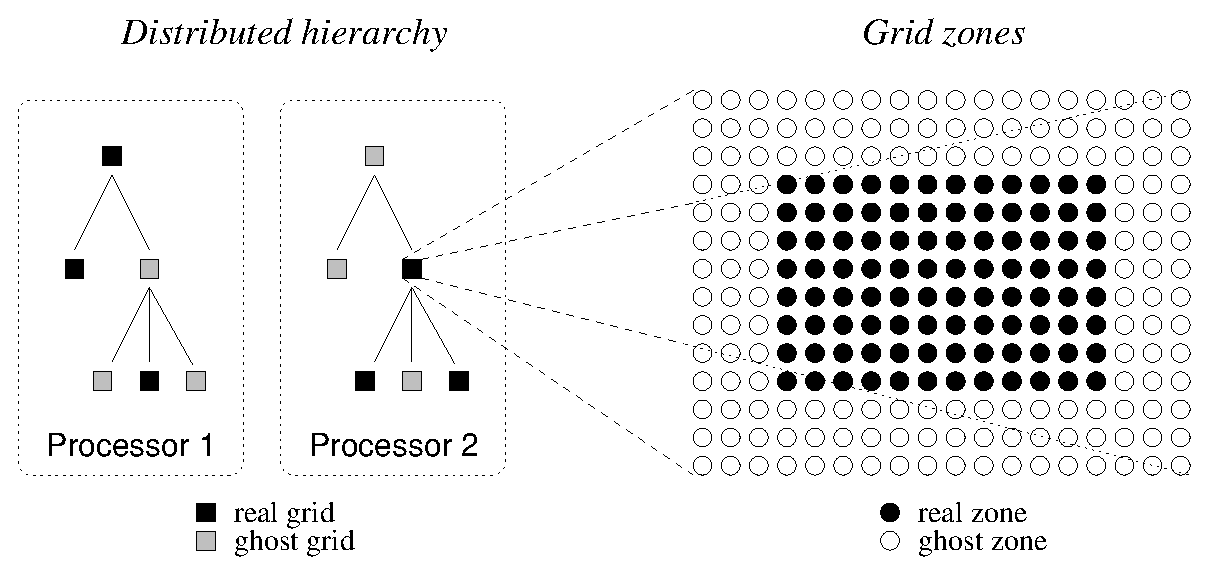
\includegraphics[width=0.5\textwidth]{figures/amr_hierarchy.eps}
\end{center}
\caption{\emph{Left:} Example of a simple, distributed AMR hierarchy
showing real and ghost grids.  \emph{Right:} Example 2D \enzo\ grid
showing real and ghost zones, as needed for the PPM hydro stencil. }
\label{fig.amr_hierarchy}
\end{figure}

Each grid patch in \enzo\ contains arrays of values for baryon and
particle quantities.   Grids are partitioned into a core of
\emph{active zones} and a surrounding layer of \emph{ghost zones}, as
shown in Figure~\ref{fig.amr_hierarchy}.  The active zones store field
values and ghost zones are used to temporarily store values that have
been obtained directly from neighboring grids or interpolated from a
parent grid.  These zones are necessary to accommodate the
computational stencil of the (magneto)hydrodynamics solvers
(Sections~\ref{sec.hydro.ppm} through~\ref{sec.hydro.zeus}) and the
gravity solver (Section~\ref{sec.gravity}).  The PPM and \zeus\ hydro
solvers require 3 layers of ghost zones,  and the gravity solver
requires 6 (although only for the density and potential fields).  This
can lead to significant memory and computational overhead,
particularly for smaller grid patches at high levels of refinement.  


From the point of view of the hydro solver, each grid is solved as an
independent computational fluid dynamics (CFD) problem, with Dirichlet
boundary conditions stored in the ghost zones.  At the beginning of
each timestep, cells on a given level fill ghost zones by
interpolating from the parent and copying from neighbors on the same
level.  Grids then correct the flux at the interface boundary between
fine and coarse zones, and finally project their active zone data to
the parent grid. 

\begin{figure}
\begin{center}
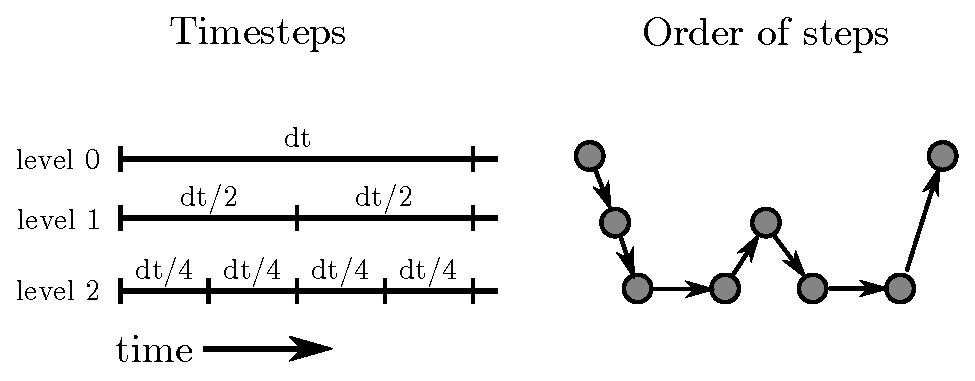
\includegraphics[width=0.6\textwidth]{figures/timestepping.eps}
\end{center}
\caption{\emph{Left:} Example of the timesteps on a 2-level AMR
  hierarchy.  \enzo\ does not restrict the timesteps on the finer levels
  to be a factor of $1/2^n$ smaller.  \emph{Right:} The order in which
  the AMR grids are evaluated on each level.\vspace{1ex}}
\label{fig:wcycle}
\end{figure}

Timesteps are determined on each level as described in
Section~\ref{sec.timestepping}, and the hierarchy is advanced on a
level-by-level basis in a W-Cycle.  Beginning with the coarsest level,
$l$, all grids on that level are advanced one timestep.  Then, one
timestep is taken on all grids at the next level of refinement, $l+1$,
and so on until the finest level is resolved. The finest level is then
advanced, using as many steps as it takes to reach the level
immediately above.  The finest level is then synched to the level
above it, which then proceeds forward in time one more step.  This is
shown graphically in Figure~\ref{fig:wcycle}.


At the end of every timestep on every level, each grid updates its
ghost zones by exchanging information with its neighboring grid
patches (if any exist) and/or by interpolating from a parent grid.  In
addition, cells are examined to see where refinement is required and
the entire grid hierarchy is rebuilt at that level (including all more
highly refined levels).  The timestepping and hierarchy
advancement/rebuilding process described here is repeated recursively
on every level to the specified maximum level of refinement in the
simulation.

The basic control algorithm looks very much like any used in a
grid-based code of a single resolution, and can be written
schematically as:

\begin{verbatim}
InitializeHierarchy
While (Time < StopTime):
   dt = ComputeTimeStep(0)
   EvolveLevel(0, dt)
   Time = Time + dt
   CheckForOutput(Time)
\end{verbatim}

The AMR control algorithm is contained within the recursive
EvolveLevel algorithm, which takes the level upon which to operate as
an argument.  This looks something like the following pseudo-code:

\begin{verbatim}
EvolveLevel(level):
   SetBoundaryValues
   while (Time < ParentTime):
      dt = ComputeTimeStep(level)
      SolveHydroEquations(dt)
      SolveOtherEquations(dt)
      Time = Time + dt
      SetBoundaryValues
      EvolveLevel(level+1, dt)
      FluxCorrection
      Projection
      RebuildHierarchy(level+1)
\end{verbatim}

Each function operates on all the grids on the given level.  In the
following sections, we will address each of the major elements in
turn.


\subsection{Setting the boundary values}
\label{sec:interpolation}

In order to solve the hydrodynamic equations on a patch, it is
necessary to specify the boundary conditions on that patch.  There are
two cases.  The first is that the boundary is external to the
computational domain.  This occurs for all the boundaries of the root
grid.  The second possibility is that the boundary is within the
computational domain, which is true for most, but not all, subgrids.


In the first case, we allow for four types of boundary conditions (for
simplicity, represented here as being at $x=0$, with positive $x$
interior and negative $x$ exterior to the domain):

\begin{enumerate}
  \item{\em Reflecting.} In this case, the boundary behaves like a
    mirror, with the solution on the boundary reflecting the solution
    in the computational domain ($q(-x) = q(+x)$) but with the
    velocity normal to the boundary reversed: $v_x(-x) = -v_x(+x)$.
  \item{\em Outflow.}  We approximate outflow boundary conditions by
    duplicating the solution at the edge of the computational domain:
    $q(-x) = q(0)$.
  \item{\em Inflow.} In this case, the boundary values are fixed by a
    pre-determined function ($q(-x) = q0(-x,t)$).  The code provides a
    simple way to set inflow values that are constant in both time and
    space over an entire face, or hooks are provided for special cases
    where the boundary must be time-varying.
  \item{\em Periodic.} The boundary solution is obtained from the
    other side of the grid: $q(-x) = q(x_{\rm{max}}-x)$.
\end{enumerate}

In the second case, the value must be either (1) interpolated from a
parent or (2) copied from a sibling.  In practice, we solve this
problem by first interpolating all boundaries from the grid's parent
and then performing the sibling copy wherever possible, since these
values will always be as good as, or superior to, interpolation.

We focus first on conserved, cell-centered quantities.  The
interpolation function should be conservative in the sense that the
mean over the interpolated quantity, in a given cell, must return the
cell-centered value.  It should also be monotonic, so that new extrema
are not introduced into a smoothly varying field.

In one dimension, such functions are well known; examples include
donor cell, Van Leer, and piecewise parabolic interpolation, which are
first-, second-, and third-order accurate respectively
\citep[e.g.,][]{Stone92a}.  However, we require fully
multi-dimensional interpolation functions, and so focus on
second-order schemes since they are tractable and relatively
accurate\footnote{We could, in principle, build a multi-dimensional
interpolator out of a one-dimensional interpolation function; however,
at higher order, this would not necessarily satisfy our constraint
regarding not introducing new extrema in interpolated quantities.}.
In Appendix~\ref{app:interpolation}, we explicitly write down
functions in one, two and three dimensions, but here we discuss the
general design considerations.

In two dimensions, it is relatively easy to build a linear, monotonic,
conservative function by requiring, first, that the function at the
center of the cell return the cell-centered quantity (and since it is
linear, this implies that an average over the cell will also be equal
to this value), and second, by treating the cell-diagonals as
one-dimensional Van Leer-type functions.  The reason to focus on the
cell diagonals is that for a linear function, the extrema will occur
at the cell corners, which are in turn linked by the diagonals.  This
process can be done in two dimensions since there are three
constraints (one at the center and one along each diagonal), and three
parameters in a two-dimensional linear function.

In three dimensions this process breaks down since the number of
constraints (center + four diagonals = five) exceeds the number of
parameters (four).  One way to solve this problem would be to perform
a least-squares fit under the given constraints; however, this is too
computationally expensive.  Therefore, in
Appendix~\ref{app:interpolation} we describe a heuristic approach that
satisfies four constaints analytically and then adjusts the
interpolation parameters in such a way as to satisfy the fifth.  While
the result is not necessarily optimal, it does appear to perform
adequately in our tests.

\subsection{Solving the hydrodynamic equations on a grid}
\label{sec:solve_hydro}

Given the grid and its boundary conditions, the process of solving
equations~(\ref{eq:mass})--(\ref{eq:total_energy}) can be detached
from the rest of the SAMR technique, so that it is possible to
experiment with a number of different methods.  The restrictions are
that the method should be flux-conservative, or at least produce an
accurate estimate of the flux of conserved quantities at cell
interfaces.  This is required in the flux-correction step (see
\ref{sec:flux_correction}).  There is also the issue of centering,
which refers to the position of physical quantities within a cell (the
primary types are cell-centered, face-centered, and node-centered).
The interpolation step, described in Section~\ref{sec:interpolation},
must correctly interpolate with the selected centering.

\subsection{Projection}
\label{sec:projection}

Since a refined region is simulated with (at least) two different
resolutions (one fine and one coarse), it has two or more
``solutions'' (i.e.~values of density, velocity, etc.) that represent
the same volume of space.  This is one important aspect of the SAMR
method -- some physical regions are represented by grids at multiple
resolutions.  To maintain consistency, the coarse grid quantities are
updated with the finer values, using a volume-weighted average of the
conserved quantities:

\begin{equation}
q^{\rm coarse} = r^{-d} \sum q^{\rm fine}_{i, j,k}
\end{equation}

where $r$ is the refinement factor, and the sum is over all fine cells
that ``cover" the coarse cell. The exponent, $d$, refers to the weight
of the average.  For cell-centered quantities, this is the
dimensionality of the problem.  For face-centered quantities, this is
one less than the dimensionality, and for edge-centered quantities
this is one.

\subsection{Flux correction}
\label{sec:flux_correction}

One of the significant advantages of flux-conservative methods is, of
course, their ability to maintain conserved quantities to machine
precision.  Unfortunately, the projection step upsets this flux
conservation since, at the boundary of a refined region, the coarse
and fine cells on either side of the border are updated with different
estimates of the flux across the boundary.  At one refinement level
this comes from the coarse grid computation, and in the other from the
fine grid solution.  Conservation can be restored by correcting all
coarse cells that lie outside the boundary of a fine region with the
difference between the coarse and fine estimates of the flux across
the boundary:

\begin{equation}
  q^{\rm coarse} = \tilde{q}^{\rm coarse} - \Delta t \left( F^{\rm
      coarse} - \sum_{j,k} F^{\rm fine}_{j,k} \right)
\end{equation}

where $F$ is the flux of quantity $q_i$ in the $i$-direction through
the cell interface.   We use $\tilde{q}$ to indicate the uncorrected
quantity on the coarse grid and the sum is over the $r^{d-1}$ fine
cell interfaces in the perpendicular dimensions that share a face with
the coarse cell being corrected.  This correction is carried out for
all coarse cells that share a face with a refined cell (and are not
themselves covered with more refined cells).

\subsection{Hierarchy reconstruction}
\label{sec:hierarchy_reconstruction}

Since the addition of more highly refined grids is adaptive, the
conditions for refinement must be specified. Many different criteria
can be simultaneously specified for a given simulation, and these
refinement criteria are discussed in more detail in the following
section (Section~\ref{sec:refinement_criteria}).   Once all cells in a
given grid that require additional refinement have been flagged,
rectangular boundaries are determined that minimally encompass the
flagged cells.  This is done using an iterative machine-vision
technique, as described in \cite{Berger91}.

We first find the smallest region (or ``proto-subgrid") that covers
all of the refined cells on a grid.  We compute an efficiency
$\epsilon$ for this grid, defined as the ratio of flagged cells to
total cells.  If this efficiency is sufficiently large (typically over
30\%), or if the grid is small enough, then we adopt the region as a
new grid and move on to the next region (if any).  If the region is
not acceptable, then we split it into two using the following
algorithm.  First, we determine the longest dimension and compute the
signature along that dimension.  The signature is found by summing the
number of refined cells with the same index along the longest
dimension.  Edges are typically indicated by inflection points in this
signature, so we calculate the second derivative using a simple
three-point finite difference estimator and look for the maximum in
the second derivative, with ties going to the index closest to the
center.  If no inflection points are found along the longest axis, the
next-longest axis is searched.  If no inflection points are found, the
longest axis is cut in half.  The original region is then split into
two new regions, or proto-subgrids.  This process is then re-applied
to each of the new regions.

This algorithm is not necessarily optimal, but experience shows it
does a reasonable job of generating an efficient covering of the
refined cells.  Note that some cells are unnecessarily refined with
the SAMR approach, resulting in wasted resources (unlike in
cell-splitting AMR schemes).  However, it has a number of advantages.
First, traditional grid-based hydro methods can be simply added with
only minor modifications.  Second, it is easier to accommodate larger
stencils (as in PPM, which requires three boundary zones), and third,
it can be more efficient for some machines since there are more
predictable and linear memory accesses, which more efficiently use a
CPU's cache.

\subsection{Refinement criteria}
\label{sec:refinement_criteria}

In this section, we turn to the refinement criteria themselves.
Although generalized refinement criteria are available based on
estimators for the error, such as the Richardson method
\citep{AtkinsonHan2004}, we have focused generally on methods that use
physical estimators based on the assumption that the simulator has a
specific quantity or quantities that indicate the need for refinement.
The flagging methods currently built into \enzo\ are:

\begin{enumerate}

\item{\em Slope.}  If the normalized slope $(q_{i+1} - q_{i-1})/ (2
  q_i)$ of baryon quantities between adjacent cells is larger than a
  specified value (typically 0.3), then the cell is flagged.

\item{\em Baryon mass.}  This refinement criterion is designed to
  mimic a Lagrangian method in that it tries to keep a fixed mass
  resolution.  In this method, a cell is refined if the baryonic mass
  in the cell ($M_g = \rho\, (\Delta x)^d$) is larger than a specified value:

\begin{equation}
M_g > \rho_{\rm flag}\, (\Delta x_{\rm root})^d r^{\epsilon_l l},
\end{equation}

where $\rho_{\rm flag}$ is the equivalent density on the root grid
required for refinement, $\Delta x_{\rm root}$ is the root grid cell
spacing, $r$ is the refinement factor, $l$ is the level and
$\epsilon_l$ is a parameter that can be used to make the refinement
more aggressive ($\epsilon_l < 0$) or less aggressive ($\epsilon_l >
0$) than pure Lagrangian refinement --- in other words,
super-Lagrangian or sub-Lagrangian refinement.

\item{\em Shocks.}  In this method, we identify and refine cells that
  contain shocks using the following criteria:

\begin{eqnarray}
(p_{i+1} - p_{i-1})/\min(p_{i+1}, p_{i-1}) > 0.33,  \qquad
u_{i-1} - u_{i+1} > 0, \quad\text{and} \qquad
e_i / E_i > 0.1.  \nonumber
\end{eqnarray}

We note that the parameters $0.33$ and $0.1$ in the equations above
were determined empirically, and can be modified by the user to refine
more or less aggressively, as the situation warrants.

\item{\em Particle mass.}  This refinement criterion is precisely the
  same as the baryon mass criterion except that it uses the gridded
  (cloud-in-cell, or CIC) particle density.  In general, this criteria
  is used in cosmological simulations, and thus refines on dark matter
  and stellar density.


\item{\em Jeans length.}  Following \cite{Truelove98}, the code can be
  forced to refine the Jeans length by a fixed number of cells, or,
  more specifically, whenever the following criterion is not met:

\begin{equation}
\Delta x < \left( \frac{\gamma \pi k_B T}{N_J^2 G \rho \mu \mh} \right)^{1/2},
\end{equation}
where $N_J$ is the required number of cells per Jeans length (4 by default).

\item{\em Cooling time.}  Often in cosmological simulations, cooling
  is a rapid process and we do not necessarily want to be limited by
  the cooling time.  However, in some cases it is desirable to resolve
  the cooling process, in which case we flag cells that have a cooling
  time shorter than their sound crossing time.  The cooling time is
  given by $t_{\rm cool} = 1.5 k_BT / (n\, \Lambda(T))$ and the sound
  crossing time is $t_{\rm cross} = \Delta x / c_s$, where $c_s$ is
  the sound speed.


\item{\em Must-refine particles.}  In order to allow for refinement in
  moving regions, it is possible to generate ``must-refine" particles
  that ensure local refinement of the 8 nearest cells to a specific
  level.  The particles feel gravitational forces and their
  trajectories are followed as for any other collisionless particle.
  This feature can be used to ensure that a specific Lagrangian region
  stays refined to a specified level of resolution. 


\item{\em Shear.} As described in \citet{Kritsuk06}, turbulence
  calculations can be successfully modeled with AMR if the shear is
  used as a refinement parameter; in particular, refinement occurs
  when the finite difference version of the following inequality
  holds:

\begin{equation}
\sum_i \sum_j \left( \frac{\partial v_i}{\partial x_j} \right)^2 -  \sum_i \left( \frac{\partial v_i}{\partial x_i} \right)^2
> \epsilon_s \frac{c_s^2}{\Delta x^2},
\end{equation}
where $\epsilon_s$ is a dimensionless parameter.

\item{\em Optical depth.} This refinement criterion, typically used
for simulations using radiation transport, flags cells for refinement
if they have an \ion{H}{1} optical depth lower than unity.  The
optical depth of a cell is estimated to be:

\begin{equation}
\tau = \sigma_{\rm HI} n_{\rm HI} \Delta x 
\end{equation}

where $\sigma_{\rm HI}$ is the neutral atomic hydrogen absorption
cross section, $n_{\rm HI}$ is the proper \ion{H}{1} number density,
and $\Delta x$ is the cell width (which is assumed to be the same
along each axis).  If $\tau > 1$, the cell is refined further, up to
the maximum level of refinement.

\item{\em Resistive length.}  In a way similar to the Jeans length
  criterion described above, the code can be forced to locally resolve
  the resistive length scale by a minimum of a fixed number of cells.
  This is done by ensuring that the resistive length scale, defined as

\begin{equation}
L_R = |B| / |\curl B|
\end{equation}

is always refined by at least N$_R$ cells locally (i.e.~we refine a
given cell further if $L_R \leq N_R \Delta x$).  Note that \enzo\ does
not actually solve the resistive MHD equations -- this is the
``characteristic'' local resistive length, rather than one calculated
within the MHD solver.

\item{\em Must refine region.}  This refinement criterion is used to
  ensure that all cells in a given subvolume of the simulation are
  refined to {\it at least} some minimum level of refinement.  The
  subvolume is user-specified, and may evolve over time (e.g., to
  follow a structure of interest that is traveling through the
  simulation volume).

\item{\em Metallicity.}  This refinement criterion ensures that all
  cells with a metallicity (defined as $Z \equiv \rho_{Z} / \rho_{b} /
  0.022$, where $\rho_{Z}$ is the density of metals in the cell,
  $\rho_{b}$ is the total baryon density (including metals), and 0.022
  is the solar mass fraction of metals) above a user-defined value is
  refined to {\it at least} some minimum level of refinement. 

\item{\em Second Derivative.}  This is similar to the refinement criteria used
  in Paramesh and was originally developed by \cite{1987nasa.reptQ....L}.  This
  method calculates the second derivative of a user-defined field normalized by
  the first derivative, and sets a threshold for refinement.  More background
  information can be found in the FLASH4 user guide\footnote{\url{http://flash.uchicago.edu/site/flashcode/user\_support/flash4\_ug/}},
  but we reproduce the relevant equation here for completeness. The
  multi-dimensional version of the criteria takes in to account all
  cross-derivatives, and is expressed by

 \begin{equation}
   S = \left\{ \frac{\sum_{ij}\left( \frac{\partial^2f}{\partial x_i \partial x_j} \right)^2}{\sum_{ij}\left[ \frac{1}{2\Delta x_j}\left( \abs{\frac{\partial f}{\partial x_i}}_{x_i+\Delta x_i} + \abs{\frac{\partial f}{\partial x_i}}_{x_i-\Delta x_i} \right) + \epsilon \frac{\abs{\bar{f_{ij}}}}{\Delta x_i \Delta x_j} \right]^2} \right\}^{1/2},
   \label{eq:second-deriv_analytical}
 \end{equation}

  where $f$ is the user-defined field, $\abs{\bar{f_{ij}}}$ is an average of
  $f$ over cells in the $i$ and $j$ dimensions, and $\epsilon$ is
  a user-controlled value that provides a method of ignoring small
  fluctuations, set by default to $10^{-2}$.  If $S$ is larger than a specified
  threshold (bounded by [0,1]) a cell is marked for refinement. This threshold
  is chosen at runtime and can vary for each of the fields under consideration.

\end{enumerate}

Finally, it is also possible to specify a rectangular region that is
statically refined to a certain level.  These static refined regions
are in place throughout the simulation regardless of the grid
quantities and can be used for testing purposes, or for
multiply-zoomed initial conditions (in cosmology simulations, for
example) that would not otherwise be refined.




\section{Fluid methods}
\label{sec.fluids}

\subsection{Hydrodynamics: The PPM hydro method}
\label{sec.hydro.ppm}

One (purely) hydrodynamic method used in \enzo\ is closely based on the
piecewise parabolic method (PPM) of
\citet{1984JCoPh..54..174C}, which has been
modified for the study of cosmological fluid flows.  
\citet{1984JCoPh..54..174C} describe two variants on this method:
Lagrangian Remap and Direct Eulerian; here we use the Direct Eulerian
version which is better suited for AMR simulations.  The Lagrangian
Remap version has previously been adapted for cosmological use
as described in \citet{1995CoPhC..89..149B} and the implementation
we use here is closely based on that work.

%We can examine the structure of Equations~(\ref{eq:mass})-(\ref{eq:total_energy})
%to obtain a better understanding of the effect of each term.
%The derivatives are first order in time
%and provide us with the dependent variables that will be evaluated each
%timestep: $\rhob$, $\vecvb$, and $E$.
%
%The second term on the left hand side of each relation
%is due to our choice of Eulerian coordinates and corresponds to
%advection, the flow of conserved quantities 
%($\rhob$, $\rhob \vecvb$, and $\rhob E$) 
%across the mesh.  These will be termed the transport terms.

The first term on the right hand side of equations~(\ref{eq:momentum}) and
(\ref{eq:total_energy}) come from our choice of comoving coordinates
(a similar term also appears in equation~(\ref{eq:dm_velocity}), the velocity 
relation for the dark matter particles).  A similar term does not
appear in the mass conservation equation (\ref{eq:mass}) because
of the comoving density definition.   
We note that these expansion terms could be
eliminated entirely by the proper choice of variables (including time),
although we have not done so here, as they do not constitute a major
source of error.  
We solve these terms (for all hydro methods)
using the same technique -- they are split from the rest of the terms and
solved using an (implicit) time-centered method, which is straightforward
as there are no spatial gradients.

%
%The remainder of the right-hand side terms (due to pressure and gravity) are denoted as
%source terms.  We make these distinctions because the 
%source and transport steps will be solved in
%a self-consistent fashion by the PPM scheme while the expansion terms,
%which are spatially localized, are split off and solved in a separate step
%(as are radiative cooling, heating and other processes, if present).  

The remainder of the terms in the fluid equations
involve derivatives.  
Because we are interested in phenomena with no special geometry, we will
restrict discussion to Cartesian coordinates.
Once again we use the concept of operator splitting,
but now apply it spatially.   We can rewrite the one-dimensional (Eulerian) 
versions of equations~(\ref{eq:mass})--(\ref{eq:total_energy}) without expansion terms
in conservative form as,
\begin{eqnarray}
\frac{\partial \rho}{\partial t}  + \frac{1}{a} \frac{\partial \rho v }{\partial x}    & = &  
     0 \label{eq:mass1d} \\
\frac{\partial \rho v}{\partial t}  + \frac{1}{a} \frac{\partial \rho v^2}{\partial x}   + 
      \frac{1}{a} \frac{\partial p}{ \partial x} & = & 
      \rho \frac{1}{a} \frac{\partial \phi}{ \partial x}  \label{eq:momentum1d}  \\
\frac{\partial \rho E}{\partial t}  + \frac{1}{a} \frac{\partial \rho v E}{\partial x}  & =  &
      \rho v \frac{1}{a} \frac{\partial \phi}{\partial x}. \label{eq:total_energy1d}
\end{eqnarray}

%
Note that $x$ and $v$ refer to the one dimensional comoving position and 
peculiar velocity of the baryonic gas, and $g$ is the acceleration at the cell center.
We write this including the cosmological scale factors, but it reduces to the non-cosmological case with $a = 1$.
These equations are now in a form that can be solved by the split PPM scheme.

% ------------------------------------------------------------

%\subsubsection{The piecewise parabolic method in one dimension} % 2.2

We now restrict ourselves to the solution of equations
(\ref{eq:mass1d})--(\ref{eq:total_energy1d}), in one
dimension.  In the Direct Eulerian version of PPM, this is
accomplished by a three-step process.  First, we compute effective
left and right states at each grid boundary by constructing a
piecewise parabolic description of the primative variables ($\rho$, $u$
and $E$) and then averaging over the regions corresponding to the
distance each characteristic wave can travel ($u$, $u-c_s$ and
$u+c_s$, where $c_s$ is the sound speed).
Second, a Riemann problem is solved using these effective left and
right states, and finally the fluxes are computed based on the
solution to this Riemann problem.  This is described in detail in
\citet{1984JCoPh..54..174C}, but we will briefly outline the procedure
here both for completeness and to put the changes we will make in
context.


The Eulerian difference equations are:
%
\newcommand{\avp}[1]{\overline{#1}_{j+1/2}}
\newcommand{\avm}[1]{\overline{#1}_{j-1/2}}
\begin{equation}
\rho_j^{n+1} = \rho_j^{n} + \Delta t \left( 
                      \frac{ \avp{\rho}\avp{v} -  \avm{\rho}\avm{v} } {\Delta x_j}
            \right)
     \label{eq:mass_diff}
\end{equation}
\begin{equation}
\rho_j^{n+1} v_{j}^{n+1} =
       \rho_j^{n+1} v_j^n  + \Delta t \left(
          \frac{ \avp{\rho} \avp{v}^2 - \avm{\rho} \avm{v}^2 + \avp{p} - \avm{p}} {\Delta x_j}
             \right)
     + \frac{ \Delta }{2} g_j^{n+1/2} (\rho_j^n + \rho_j^{n+1}), 
     \label{eq:momentum_diff}
\end{equation}
\begin{eqnarray}
\rho_j^{n+1} E_j^{n+1}  = 
       \rho_j^n E_j^n  & + & \Delta t  \left(
            \frac{  \avp{\rho} \avp{v} \avp{E}  - \avm{\rho} \avm{v} \avm{E}  +
                       \avp{v} \avp{p}    - \avm{v} \avm{p} } {\Delta x_j}
             \right) \nonumber \\
         & & + \frac{ \Delta t }{2} g_j^{n+1/2} (\rho_j^n v_j^n + \rho_j^{n+1} v_j^{n+1} ).
     \label{eq:energy_diff}
\end{eqnarray}

We have used subscripts to indicate zone-centered ($j$)
and face-centered ($j+1/2$) quantities, while superscripts refer to
position in time.  The cell width is $\Delta x_j$.
Although they have been discretized
in space, the accuracy of the updates depend on how well we can compute
the fluxes into and out of the cell during $\Delta t$.  
This in turn depends on our ability to compute the time-averaged 
values of $p$, $\rho$ and $v$ at the cell interfaces, denoted here
by $\overline{p}_{j\pm 1/2}$, $\overline{\rho}_{j\pm 1/2}$, and $\overline{v}_{j\pm 1/2}$.  We now
describe the steps required to compute these quantities.

We first construct monotonic piecewise 
parabolic (third order) interpolations in one dimension
for each of $p$, $\rho$, and $v$.  The pressure is determined from
equation~(\ref{eq:eq_of_state}), the equation of state.
%We have dropped the subscript b in this and the following two sections because we will be referring solely to baryonic quantities.  
The interpolation formula for some quantity $q$ is given by:
%
\begin{eqnarray}
q_j(x) & = &  q_{L,j} + \tilde{x}(\Delta q_j + q_{6,j}(1-\tilde{x})), \\
\tilde{x}      & \equiv & {x - x_{j-1/2} \over \Delta x_j}, \qquad
             x_{j-1/2} \leq x \leq x_{j+1/2}. \nonumber
\end{eqnarray}
%
This is Equation~(1.4) of CW84 (in the spatial rather than mass coordinate as is appropriate for the direct Eulerian approach). 
%The zones edges in the mass coordinates are $m_{j-1/2}$ and $m_{j+1/2}$ for the left and right edges, respectively.  
The quantities $q_{L,j}$, $\Delta q_j$,
and $q_{6,j}$ can be viewed simply as interpolation constants; however,
they also have more intuitive meanings.  For example, $q_{L,j}$ is the
value of $q$ at the left edge of zone j, while $\Delta q_j$ and $q_{6,j}$ are analogous to the slope and first order correction to the slope of $q$ (see \citet{1984JCoPh..54..174C} for a complete discussion):
\begin{equation}
\Delta q_j \equiv q_{R,j} - q_{L,j} \qquad 
q_{6,j}    \equiv 6\left[q_j - 1/2\left(q_{L,j} + q_{R,j}\right)\right].
\end{equation}

We have reduced the problem to finding $q_{L,j}$ and $q_{R,j}$.  While this
is simple in principle, it is complicated somewhat by the requirement that
these values be of sufficient accuracy and that the resulting distribution
be monotonic.  That is, no new maxima or minima are introduced.
The resulting formulae are straightforward but complicated and are not
reproduced here, but see Equations 1.7 to 1.10 of \citet{1984JCoPh..54..174C}.
We also optionally allow steepening as described in that reference.

Once we have the reconstruction, the primary quantities ($p$, $\rho$, $v$ and $E$) are averaged over the domains corresponding to the three characteristics $C = u-c$, $u$ or $u+c$ (where $c$ is the sound speed in a cell):
\begin{eqnarray}
      q^{C+}_{j+1/2} & = &
          {1 \over \Delta t C^n_j} \int^{x_{j+1/2}}_{x_{j+1/2}-\Delta t C^n_j} q_j(x) dx, \\
      q^{C-}_{j+1/2} & = & 
         {1 \over -\Delta t C^n_{j+1}} \int^{x_{j+1/2}+\Delta t C^n_{j+1}}_{x_{j+1/2}} q_{j+1}(x) dx \nonumber
\end{eqnarray}
where $q^{C+}$ ($q^{C-}$) refers to the left (right) characteristic $C$.  The linearized gas dynamics equations are then used to compute second-order accurate left and right states that take into account the multiple wave families.  This process is described in \citet{1984JCoPh..54..174C} and we use their equations (3.6) and (3.7).

With these effective states, an approximation to the Riemann problem is found
with an iterative approach \citep[see][and section~\ref{sec.riemann}]{Woodward86}, producing estimates for 
$\overline{p}_{j\pm 1/2}$, $\overline{\rho}_{j\pm1/2}$, and $\overline{v}_{j\pm 1/2}$ that are third order
accurate in space and second order accurate in time.  These are then
used to solve the difference Equations (\ref{eq:mass_diff})--(\ref{eq:energy_diff}) for $\rho^{n+1}$, $v^{n+1}$, and $E^{n+1}$.

We include an optional diffusive flux (and flattening for the parabolic curves) that can improve the solution in some cases.  Our implementation follows that in the appendix of \citet{1984JCoPh..54..174C}.

In addition, as discussed earlier, the three dimensional scheme is achieved by operator splitting and repeating the above procedure in the other two orthogonal directions.  The transverse velocities and any additional passive quantities are naturally and easily added to this system (see Equation 3.6 of \citet{1984JCoPh..54..174C}).  

We note that the acceleration required in Equation~(\ref{eq:momentum_diff}) is actually the
acceleration felt by the entire zone and not just at the zone center.
Therefore, it is possible to find the mass weighted average acceleration over the zone
by expanding the density and acceleration distributions and
retaining all terms up to second order in $\Delta x$:
%
\begin{equation}
g_j^{n+1/2} = 
       \frac{1}{2 a^{n+1/2} \delta x_j} \left[ 
             \phi_{j+1}^{n+1/2} 
           - \phi_{j-1}^{n+1/2} 
           + \frac{1}{12} \left(    \phi^{n+1/2}_{j+1} 
                                 - 2\phi^{n+1/2}_j 
                                 + \phi^{n+1/2}_{j-1} \right) 
                                   {\delta d_j \over d_j}
       \right].
       \label{eq:accel}
\end{equation}
Generally we find that the potential is so slowly varying that this change is unnecessary.

% ------------------------------------------------------------

\subsubsection{The dual energy formulation for  very high Mach flows} % 2.4

The system described thus far works well for gravitating systems with
reasonable Mach numbers ($<100$) as long as the structures are well resolved.
This section and the next detail changes that are required
to correctly account for situations where one or both of these
requirements are not met.

Large, hypersonic bulk flows appear to be very common in cosmological
simulations and they present a problem because of the high ratio of
kinetic energy $E_k$ to gas internal energy $e$, which can reach as
high as $10^8$.  Inverted, we see that the internal energy consists of
an extremely small portion of the total energy.  The pressure then,
proportional to $E - E_{k}$, is the small difference between two large
numbers: a disastrous numerical situation.  This is not as large a
problem as it may at first appear because it only occurs when the
pressure is negligibly small.  Therefore, even if we suffer large
errors in the pressure distribution in these regions, the dynamics and
total energy budget of the flow will remain unaffected.  Nevertheless,
if the temperature distribution is required for other reasons
(e.g., for calculating radiative processes), a remedy is required.

To overcome this, we also solve the internal energy equation:
\begin{equation}
 \frac{\partial e}{\partial t} 
           + \frac{1}{a} \vecv \cdot \grad e
%         = - \frac{3(\gamma -1)\dot{a}}{a} e
         = - 3 \frac{\dot{a}}{a} \frac{p}{\rho}
           - \frac{p}{a\rho} \div \vecv
\end{equation}
in comoving coordinates.  The structure is similar to the total energy
equation; the second term on the left hand side represents transport, while
the first term on the right is due to expansion of the coordinate
system.  
It is differenced (again, in Eulerian form without the expansion term) as,
%
\begin{equation}
\rho_j^{n+1} e_j^{n+1}  = 
       \rho_j^n e_j^n   +  \Delta t  \left(
            \frac{  \avp{\rho} \avp{v} \avp{e}  - \avm{\rho} \avm{v} \avm{e}} {\Delta x_j} \right)
            - \Delta t \ p_j^{n} \left( \frac{ \avp{v} - \avm{v}} {\Delta x_j} 
                      \right)
                  \label{eq:gasenergy_diff}
\end{equation}
%
Note that because of the structure of this equation, it is not in
flux-conservative form.  In particular, the pressure is evaluated at
the cell center.  Unfortunately, time-centering of this pressure has
proved difficult to do without generating large errors in the internal
energy and so we leave the pressure at the old time in
this difference equation.  This leads to some spreading of shocks; however,
we note that this equation is only used in hypersonic flows.

It is necessary, however, to conserve the total energy so that the conversion
of kinetic to thermal energy is performed properly.   We must therefore,
combine the two formulations without allowing the separately advected
internal energy $e$ to play a role in the gas dynamics.  This is done by
carrying both terms through the simulation and using
the total energy $E$ for hydrodynamic routines and the internal energy
$e$ when the temperature profile is required.  One way to view this procedure
is to treat $e$ as enhanced precision (extra digits) for $E$ that automatically
`floats' to where it is needed.
We only require that they be kept synchronized when the two levels of precision
overlap.

When the pressure is required solely for dynamic purposes, the 
selection criterion 
operates on a cell by cell basis using,
\begin{equation}
p = \cases{ \rho(\gamma - 1)(E - \vecv^2/2),& 
                  $  (E - \vecv^2/2)/E > {\eta}_1 $; \cr
            \rho(\gamma -1)e,&
                  $  (E - \vecv^2/2)/E < {\eta}_1 $. \cr}
\end{equation}

It should be stressed that as long as the parameter ${\eta}_1$ is small enough
the dual energy method {\it will have no dynamical effect}.  We use
${\eta}_1 = 10^{-3}$, which is consistent with the truncation error of the
scheme for grid sizes that are typically used in our simulations.  We are now free to select the method by which the internal energy
field variable $e$ is updated so that it will not become contaminated with
errors advected by the total energy formulation but still give the
correct distribution in shocked regions. 
Since we are concerned with the advection of errors, the selection
criterion must look at each cell's local neighbourhood.
In one dimension, this is done with,
\begin{equation}
e = \cases{ (E - \vecv^2/2),& $\rho(E - \vecv^2/2)/
    \max ({\rho}_{j-1}E_{j-1},{\rho}_j E_j,{\rho}_{j+1}E_{j+1}) > {\eta}_2$,\cr
            e,& $\rho(E - \vecv^2/2)/
    \max ({\rho}_{j-1}E_{j-1},{\rho}_j E_j,{\rho}_{j+1}E_{j+1}) < {\eta}_2$.\cr}
    \label{eq:dualselect}
\end{equation}
Thus, ${\eta}_2$ determines when the synchronization (of $e$ with $E$) occurs.
%is a measure of how much error we will allow to be passed
%from neighboring cells.  
Too high a value may mask relatively weak shocks, 
while spurious heating (via contamination) may occur if it is set too low.
After some experimentation,
we have chosen ${\eta}_2 = 0.1$, a somewhat conservative value.
This scheme is optional and is generally only required in large-scale 
cosmological simulations where the gas cools due to the expansion of the universe
but large bulk flows develop due to the formation of structure.

We note that others have independently developed a similar but
distinct scheme for dealing with this problem, which is endemic to
methods adopting the total energy equation.  In \citet{TVD93} the 
two variables adopted are total energy and
entropy (rather than total energy and thermal energy), with an
analogous scheme for choosing which variable to employ.

\subsubsection{Riemann Solvers and Fallback}
\label{sec.riemann}

While most numerical hydrodynamics schemes center around finding approximate
solutions to the hydrodynamics equations, the core philosophy of a Godunov
method \citep{Godunov1959} is to find the exact solution to an
approximation of the physical setup.  The approximate problem in this case is
the Riemann problem, wherein two volumes are separated by a thin membrane that
is instantaneously removed at time $t=0$.  The subsequent evolution has an exact 
analytic solution.  This solution is
described in detail in many texts on computational fluid dynamics
\citep[e.g.,][]{toro-1997}.   In brief, there are three waves that propagate
away from the initial discontinuity.  The central wave, characterized by a
density jump but not a pressure jump, is called the contact discontinuity.  The
waves traveling to the left and right of the contact discontinuity can be either
shocks, if characteristics converge on the wave front, or  rarefaction fans if
characteristics diverge.  

While there exists an exact solution to this problem, finding it is expensive.  There are four
possible combination of left- and right- traveling shocks and rarefactions,
only one of which is fully consistent with the initial conditions.  Once the
correct physical state is determined, the pressure in the central region can
only be found by finding the root to an algebraic equation, which is necessarily
an iterative process.  Thus a series of \emph{approximate} Riemann solvers are
typically used.  There are four approximate Riemann solvers in \enzo: two-shock
\citep{toro-1997},
Harten-Lax-van Leer \citep[HLL,][]{toro-1997}, HLL with a contact discontinuity
 \citep[HLLC,][]{toro-1997}, and HLL with
multiple discontinuities \citep[HLLD,][]{Miyoshi05}.  Two-shock is used only
with the PPM method.  HLL and HLLC are used with PPM, MUSCL (both with and
without MHD) and MHD-CT.  HLLD is exclusively an MHD solver, and works with both
MUSCL and MHD-CT methods.  

The only approximation that two-shock makes is that both left- and right- moving
waves are shocks.  This solution still requires an iterative method for finding
the pressure in between the two waves.  The HLL method alleviates this iteration
by assuming that there is no central contact discontinuity, and the signal speed
in the central region is approximated by an average over the left- and right-
moving waves.  This method is significantly faster than the two-shock method,
but also quite a bit more dissipative.  The HLLC is a three-wave method that improves upon the HLL
method by also including the third wave, the contact discontinuity.  

For the MHD equations, there are seven waves, instead of three.  This makes the
exact solution to the Riemann quite a bit more expensive.  Both the HLL and HLLC
approximations can be formulated for the MHD equations, and are employed in both
the Dedner and CT solvers in \enzo.  The HLLD
solver includes two of the additional waves, the rotational discontinuities,
making it a five-wave solver.

On rare occasions, high order
solutions can cause negative densities or energies.  Both PPM and MUSCL solvers employ a Riemann
solver fallback mechanism \citep{Lemaster09}.  If a negative density is found at
a particular interface, the more diffusive HLL Riemann solver is used to compute the fluxes associated with that cell.




\subsection{Hydrodynamics: MUSCL}
\label{sec.num.hydro-muscl}

The second method we describe is a MUSCL-based solver than can be used in both HD and MHD modes.  The description here will be very brief both because the ideas are similar to those described in the previous section, and because this implementation has previously
been described in more detail elsewhere \citep{WangAbelZhang08, WangAbel09}.

Much like the PPM solver, we have three basic steps: the first is
reconstruction of the variables, the second is a solution of the
Riemann problem, and the third is is updating the conserved quanties
with the fluxes as written above.
For the reconstruction scheme we have implemented only the simple
piecewise linear reconstruction \citep{1979JCoPh..32..101V, 1985JCoPh..59..264C},
with options for both primitive and conservative variable reconstruction.
The available Riemann solvers are HLL, HLLC, and HLLD, as described earlier.

To more clearly describe the Dedner divergence cleaning modifications, we write the equations of compressible inviscid hydrodynamics can be written in the form of conservation laws as,
\begin{equation}
 \frac{\partial{U}}{\partial{t}} +
 \frac{\partial{F^x}}{\partial{x}} + \frac{\partial{F^y}}{\partial{y}} + \frac{\partial{F^z}}{\partial{z}}= 0, \label{hydro}
\end{equation}
The conserved variable $U$ is given by
\begin{equation}
 U = (\rho, \rho v_x, \rho v_y, \rho v_z, \rho E)^{T},
\end{equation} 
where $\rho$ is density, $v_i$ are the three components of velocity
for $i={x,y,z}$, $E=v^2/2 + e$ denotes the specific total energy and $e$ the
specific internal energy.

For the generalized Lagrange multiplier formulation of the MHD
equations \citep{2002JCoPh.175..645D}, we consider these 
conserved variables
\begin{equation}
 U = (\rho, \rho v_x, \rho v_y, \rho v_z, \rho E+B^2/2, B_x, B_y, B_z, \psi)^{T},
\end{equation} 
where $B_i$ with $i={x,y,z}$ are the three components of magnetic
fields and $\psi$ is the additional scalar field introduced in the GLM
formulation for the divergence cleaning.  The fluxes then are
\begin{eqnarray}
 F^x &=& (\rho v_x, \rho v_x^2+p+B^2/2-B_x^2, \rho v_yv_x-B_yB_x, \cr
 && \rho v_zv_x-B_zB_x, \rho ({v^2\over2} + h)v_x+B^2v_x-B_xB\cdot v, \cr
&& \psi, v_xB_y-v_yB_x, -v_zB_x+v_xB_z, c_h^2B_x)^T,\\
 F^y &=& (\rho v_y, \rho v_xv_y-B_xB_y, \rho v_y^2+p+B^2/2-B_y^2, \cr
 && \rho v_zv_y-B_zB_y, \rho ({v^2\over2} + h)v_y+B^2v_y-B_yB\cdot v, \cr
 && v_yB_z-v_zB_y,\psi,-v_xB_y+v_yB_x, c_h^2B_y)^{T}, \\
 F^z &=& (\rho v_z, \rho v_xv_z-B_xB_z, \rho v_yv_z-B_yB_z, \rho v_z^2+p+B^2/2-B_z^2, \cr
 && \rho ({v^2\over2} + h)v_z+B^2v_z-B_zB\cdot v, \cr
    &&  -v_yB_z+v_zB_y, v_zB_x-v_xB_z,\psi, c_h^2B_z)^{T},
\end{eqnarray}
where $c_h$ is a constant controlling the propagation speed and
damping rate of $\div B$, and $h=e+p/\rho$ denotes the enthalpy.
All quantities are cell-centered.

The method is dimensionally un-split in that the fluxes are computed
for all dimensions first and the conserved quantities are updated in
one step, in contrast to the Strang splitting employed in the other solvers.
Also unlike the other schemes, time-integration is done with a second-order
Runge-Kutta scheme \citep{1988JCoPh..77..439S}.
  % includes MUSCL and Dedner
\subsection{MHD: Constrained transport}
\label{sec.num.mhd-ct}
  
\subsection{Hydrodynamics: The \zeus\ method}
\label{sec.hydro.zeus}

As an alternative to the previous Godunov methods, \enzo\ also includes an implementation of the finite difference hydrodynamic algorithm employed in the compressible magnetohydrodynamics code \zeus\ \citep{Stone92a, Stone92b}.  Fluid transport is solved on a Cartesian grid using the upwind, monotonic advection scheme of \citet{1977JCoPh..23..276V} within a multistep (operator-split) solution procedure that is fully explicit in time.  This method is formally second-order accurate in space but first-order accurate in time.  
 
As discussed in the section describing the Piecewise Parabolic Method (Section~\ref{sec.hydro.ppm}), operator-split methods break the solution of the hydrodynamic equations into parts, with each part representing a single term in the equations.  Each part is evaluated successively using the results preceding it.  In this method, in addition to operator-splitting the expansion terms (i.e., those terms in Eqs.~(\ref{eq:mass}) -- (\ref{eq:total_energy}) that depend on $\dot{a}$), we divide the remaining terms into \emph{source} and \emph{transport} steps.  The terms to be solved in the source step are those on the right-hand side of eqs.~(\ref{eq:mass}) -- (\ref{eq:total_energy}), while the transport terms are on the left-hand side of these equations and are responsible for the advection of mass, momentum and energy across the grid.

The \zeus\ method uses a von Neumann-Richtmyer artificial viscosity to smooth shock discontinuities that may appear in fluid flows and can cause a breakdown of the finite difference equations.  The artificial viscosity term is added in the source terms as:
\begin{eqnarray}
\rho \frac{\partial\vecv}{\partial t} &=& - \grad p - \rho \grad \phi 
- \div \textbf{Q} \\
\frac{\partial e}{\partial t} &=& -p \div \vecv - \textbf{Q} : \grad \vecv, 
\end{eqnarray}
Here \textbf{Q} is the artificial viscosity stress tensor, which we take to be diagonal with on-axis terms given by $l^2 \rho (\partial v / \partial x)^2$ as proposed by von Neumann \& Richtmyer.  The length scale $l$ determines the width of shocks and is typically a few times the cell spacing.

In our Cartesian coordinate system, the finite difference version of these equations is particularly simple, although there is one important complication.  In the \zeus\ formalism, the velocity is a face-centered quantity -- that is, the velocity is recorded on a grid that is staggered as compared to the density, pressure and energy, which are at the cell center.  Therefore we must remember that $v_j$ is at position $x_{j-1/2}$ (we use this notation, rather than writing $v_{j+1/2}$ both to match the original \zeus\ paper and also to make it easier to compare these equations to what is actually in the code).  

As in the original \zeus\ paper, the source terms are added in three steps. First we add the pressure and gravity forces:
\begin{equation}
v_j^{n+a}  =  v_j^n - \frac{\Delta t}{\Delta x_j} \frac{p^n_j - p^n_{j-1}} {(\rho^n_j + \rho^n_{j-1})/2}.
\end{equation}
Partial updates are denoted by the $n+a$, $n+b$ notation.  We show updates in one dimension as the extension to the multi-dimensional case is straightforward (note that all dimensions are carried out for each substep before progressing to the next substep). We then add the artificial viscosity:
\begin{eqnarray}
v_j^{n+b} & = & v_j^{n+a} - \frac{\Delta t}{\Delta x_j} 
                             \frac{q^{n+a}_j - q^{n+a}_{j-1}} {(\rho^n_j + \rho^n_{j-1})/2} \\
e_j^{n+b} & = & e_j^n - \frac{\Delta t}{\Delta x_j} q^{n+a}_j (v^{n+a}_{j+1} - v^{n+a}_{j}).
\end{eqnarray}
The artificial viscosity coefficient $q_j$ is given by:
\begin{equation}
q_j = \left\{ \begin{array}{ll}
              Q_{\rm AV} \rho_j (v_{j+1} - v_j)^2 \quad & \rm{if}~(v_{j+1} - v_j) < 0 \\
               0 & \rm{otherwise}
               \end{array} \right.
\end{equation}
where $Q_{\rm AV}$ is a constant with a typical value of 2. We refer the interested reader to \citet{Stone92a} and \citet{1994ApJ...429..434A} for more details.  We also include the option (turned off by default) of adding a linear artificial viscosity as suggested in the \zeus\ paper for stagnant flow regions.  This is given by
\begin{equation}
q_{{\rm lin},j} = Q_{\rm LIN} \rho c_j (v_{j+1} - v_{j})
\end{equation}
where $c_j^2 = \gamma p/\rho$ is the adiabatic sounds speed.

Finally, the third source step is the compression term and is given by
\begin{equation}
e^{n+c}_j = e^{n+b}_j \left( \frac{1 - (\Delta t/2) (\gamma - 1) (\div \vecv)_j }
                           {1 + (\Delta t/2) (\gamma - 1) (\div \vecv)_j } \right)
\end{equation}
We have used the notation $(\div \vecv)_j$ to indicate the (potentially) multi-dimensional velocity divergence evaluated at the cell center position $x_j$.  This equation differs from the previous ones in that in the multi-dimensional case, still only one finite difference equation is evaluated, but the divergence becomes multi-dimensional.

We next examine the transport step, which is conservative.  Once again, we dimensionally split the equations and present only the one-dimensional version.  The finite difference equations actually solved are:
\begin{equation}
\rho_j^{n+d} = \rho_j^{n} - \frac{\Delta t}{\Delta x} (v^{n+c}_{j+1/2} \rho^{*}_{j+1/2} - v^{n+c}_{j-1/2} \rho^{*}_{j-1/2} )
\end{equation}
Here $\rho^*_j$ is the correctly upwinded value of $\rho$ evaluated at the cell-face corresponding to $v_j$, making $\rho^*_j v_j$ the mass flux at the cell boundary and guaranteeing mass conservation.   This requires interpolating each cell-centered quantity to the cell edge.  As recommended in \citet{Stone92a}, we use the second-order van Leer scheme, which uses piecewise linear functions.  These are given by Equations (48) and (49) of \citet{Stone92a}.  The transport steps for the other variables are similar.  Note that we advect the specific energy and specific momenta using the mass flux, as dictated by the principle of consistent transport.  This requires appropriate averaging for the momenta in the perpendicular directions as outlined in equations (57)-(72) of \citet{Stone92a}.

%GB: the following is not correct (it is based on the Anninos & Norman paper which uses a
%GB: different set of definitions for the comoving coordinates).
%\begin{eqnarray}
%Q_{ii} & = & \left\{ 
%   \begin{array}{ll}
%      Q_{\rm AV} \rho_b  (a \Delta v_{i} + \dot{a} \Delta x_i)^2 \quad
%       & \textrm{for $a \Delta v_{i} + \dot{a} \Delta x_i < 0$}  \\
%      0 & \textrm{otherwise}\\
%\end{array} \right. \\
%%\end{eqnarray}
%%and
%%\begin{equation}
%Q_{ij} & = & 0  \;\;\;{\rm for}\;\; i \ne j . 
%%\end{equation}
%\end{eqnarray}
%$\Delta x_i$ and $\Delta v_{i}$ refer to the comoving width of the grid cell
%along the $i$-th axis and the corresponding difference in gas
%peculiar velocities across the grid cell, respectively, and $a$ is the
%cosmological scale factor.  

A limitation of a technique that uses an artificial viscosity is that, while the correct Rankine-Hugoniot jump conditions are achieved, shocks are broadened over 3-4 mesh cells. This may cause unphysical pre-heating of gas upstream of the shock wave, as discussed in \citet{1994ApJ...429..434A}.  On the other hand, it is much more robust than PPM and is easy to add additional physics.  We also note that this method solves only the internal energy equation rather than total energy, so the dual energy formulation discussed in Section~\ref{sec.hydro.ppm} is unnecessary.


\section{Gravity and N-body}
\label{sec.allgrav}
\subsection{Gravity}
\label{sec.gravity}

Solving for the accelerations for the cells and particles in a grid due to self-gravity involves three steps: first, computing the total gravitating mass; second, solving for the potential field with the appropriate boundary conditions, and finally, differencing the potential to get the acceleration and, if necessary, interpolating the potential back to the particles. These steps are described in detail below.

First, the dark matter particles are distributed onto the grids using the cloud-in-cell (CIC) interpolation technique \citet{Hockney88} to form a spatially discretized density field $\rho_{\rm DM}$.  When doing the CIC interpolation, particle positions are (temporarily) advanced by $0.5 \Delta t v^n$ so that we generate an estimate of the time-centered density field.  Particles on sub-grids are also added in this way.  In addition, since the gravitating field for a grid is defined beyond the grid edges (see below), dark matter particles from sibling grids and sub grids which lie within the entire gravitating field are used.

Next, we add the baryonic grid densities in a similar fashion.  In particular, we treat baryonic cells as virtual CIC particles which are are placed at the grid center but are advanced by $0.5 \Delta t v^n$ in order to approximately time-center the gravitating mass field.  Cells which are covered by further refined grids are treated in a similar way (i.e. we use the sub grid cells as virtual CIC particles).  This procedure results in a total gravitating mass field $\rho_{\rm total}^{n+1/2}$.

To compute the potential field from this gravitating mass field on the root grid, we use a a fast Fourier transform. For periodic boundary conditions, we can use either a simple Greens function kernel of $-k^{-2}$, or the finite-difference equivalent \citep{Hockney88}:
\begin{equation}
G(\vec{k}) = - \frac{\Delta x}{2 \left( \sin(k_x \Delta x/2)^2 + \sin(k_y \Delta y/2)^2 + \sin(k_z \Delta z/2)^2 \right) }
\end{equation}
where $k^2 = k_x^2 + k_y^2 + k_z^2$ is the wavenumber in Fourier space and the potential is calculated in k-space as usual with $\tilde{\phi}(k) = G(k) \tilde{\rho}(k)$.  

For isolated boundary conditions, we use James method (REF).  In this case, the Greens function is generated in real-space so as to have the correct zero-padding properties and then transformed into the Fourier domain.  In either case, the potential is then transformed back into the real domain to get potential values at the cell centers.  These are differenced with a two-point centered difference to get accelerations at the cell centers (except if we are using the staggered Zeus-like solver, in which case the accelerations are computed at the cell faces to match the velocities).


In order to calculate more accurate potentials on subgrids, \enzo\ re-samples the dark matter density onto individual subgrids using the same CIC method as on the root grid, but at higher spatial resolution (and again adding baryon densities if applicable). Boundary conditions are then interpolated from the potential values on the parent grid.  We use either tri-linear interpolation or a natural second-order spline: both methods seem to give similar results. The potential equation on each subgrid is then solved with the given Dirichlet boundary conditions.  This solution is done with a multigrid relaxation technique (but only applied to each subgrid).

The region immediately next to the boundary can contain unwanted oscillations (Anninos \etal REF), and so we use an expanded buffer zone around the grid, of size three root grid boundary zones (so typically six refined zones).  The density is computed in this region and the potential solved, but only the region which overlaps with the grid itself is used to calculate accelerations.

It is known (REF) that simply interpolating the potential without feeding it back to higher levels leads to errors in the potential at more refined levels because of the build-up of errors during the interpolation of coarse boundary values.  
In addition, neighboring subgrids are not guaranteed to generate the same potential values because of the lack of a coherent potential solve across the whole hierarchy. In an attempt to partially alleviate this problem, we allow for an iterative procedure across sibling grids, in which the potential values on the boundary of grids can be updated with the potential in `active' regions of neighboring subgrids.  To prevent overshoot, we average the potential on the boundary and allow for (typically) 4 iterations.  This procedure can help in many cases, but does not produce a coherent solution across all grids and so does not solve the problem; we are working on a slower but more accurate method which does a multi-grid solve across the whole grid (Reynolds \etal, in preparation).

Forces are computed on the mesh by finite-differencing potential values and are then interpolated to the particle positions, where they are used to update the particle's position and velocity information.  Potentials on child grids are computed recursively and particle positions are updated using the same timestep as in the hydrodynamic equations.  

At this point it is useful to emphasize that the effective force resolution of an adaptive particle-mesh calculation is approximately twice as coarse as the grid spacing at a given level of resolution.  
%The potential is solved in each grid cell; however, the quantity of interest, namely the acceleration, is the gradient of the potential, and hence two potential values are required to calculate this.  In addition, it should be noted that the adaptive particle-mesh technique described here is very memory intensive: in order to ensure reasonably accurate force resolution at grid edges the multigrid relaxation method used in the code requires a layer of ghost zones which is very deep -- typically 6 cells in every direction around the edge of a grid patch.  This greatly adds to the memory requirements of the simulation, particularly because subgrids are typically small (on the order of $12^3 - 16^3$ real cells for a standard cosmological calculation) and ghost zones can dominate the memory and computational 
requirements of the code.


\subsection{N-body Dynamics}
\label{sec.ov.nbody}

\enzo\ uses a particle-mesh N-body method to calculate the dynamics of
collisionless systems \citep{Hockney88}.  This method follows
trajectories of a representative sample of individual particles that
sample the phase space of the dark matter distribution, and is much
more efficient than a direct solution of the Boltzmann equation in
essentially all astrophysical situations for the levels of accuracy
that are required for simulations of structure formation.  As
described earlier, the gravitational potential is computed by solving
the elliptic Poisson's equation (Eq.~\ref{eq:potential}) and
differencing the potential to find accelerations, which are then
interpolated back to particles.  This acceleration is time-centered
(because the underlying gravitating mass field is approximately
time-centered), and so we have accelerations $\myvec{g}^{n+1/2}$ for
each particle.  These are used to update the particle positions and
velocities starting from $\myvec{x}^n$ and $\myvec{v}^n$ using a
standard drift-kick-drift technique \citep{Hockney88}:

\begin{eqnarray}
\label{eqn.driftkick}
\myvec{x}^{n+1/2} & = & \myvec{x}^n + \frac{\Delta t}{2 a^n} \myvec{v}^{n} \nonumber \\
\myvec{v}^{n+1} & = & \myvec{v}^n \left(1 - \frac{\dot{a}^{n+1/2}}{a^{n+1/2}}\right) + \frac{\Delta t}{ a^{n+1/2}} \myvec{g}^{n+1/2} \\
\myvec{x}^{n+1} & = & \myvec{x}^{n+1/2} + \frac{\Delta t}{2 a^{n+1}} \myvec{v}^{n+1} \nonumber
\end{eqnarray}

Particles are stored in the most highly refined grid patch at the
point in space where they exist, and particles that move out of a
subgrid patch are sent to the grid patch covering the adjacent volume
with the finest spatial resolution, which may be of the same spatial
resolution, coarser, or finer than the grid patch from which the
particles moved.  This takes place in a communication process at the
end of each timestep on a level.

To avoid unphysical point-mass effects, \enzo\ provides a parameter
that governs the maximum level at which particles will be regarded as
point masses.  At higher levels, contributions from particles to the
gravitating mass field will be smoothed over a spherical region
centered at each particle's position.

\section{Microphysics}
\label{sec.microphysics}
\subsection{Chemistry, radiation and cooling}
\label{sec.ov.chem}

\red{
As this stands it is the methods that I (brian) use, so I don't really emphasize
either the tabular cooling functions or the various radiation background options.
Add more discussion of this, point towards appendix.
}

Though the equations of hydrodynamics described above are a closed system,
they are still missing a crucial piece of physics: radiative heating and cooling.
Radiative cooling is extremely important in many astrophysical situations, as is 
the heating of gas from some sort of radiation background.  \enzo\ has a very simple
Sutherland and Dopita equilibrium cooling function \citep{1993ApJS...88..253S} 
implemented, which uses a
cooling table assuming a fixed metallicity of $Z = 0.3 Z_\odot$, and also a
nonequilibrium heating/cooling model that assumes gas of primordial composition exposed to a
uniform metagalactic ultraviolet (UV) background that varies with time \citep{1996ApJS..105...19K}.  

The simulations discussed in this thesis almost exclusively use the nonequilibrium
routines, described in great detail by Abel et al. and Anninos et al.  
\citep{abel97,anninos97} and summarized in Appendix~\ref{app:chemistry}. These 
routines follow the non-equilibrium chemistry of a 
gas of primordial composition with 9 total species:  
$H$, $H^+$, $He$, $He^+$, $He^{++}$, $H^-$, $H_2^+$, $H_2$, and $e^-$.  The code also calculates 
radiative heating and cooling, following atomic line excitation, recombination,
collisional excitation, free-free transitions, molecular line excitations, and Compton
scattering of the cosmic microwave background, as well as any of
approximately a dozen different models for a metagalactic UV background that heat
the gas via photoionization and photodissociation. 
The multispecies rate equations are solved out of
equilibrium to properly model situations where, e.g., the cooling rate of the gas
is much shorter than the hydrogen recombination time.  The effect of this nonequilibrium
cooling is to leave behind a much larger fraction of residual free electrons than one would
expect if the assumption of equilibrium were being made.  The practical effect of this
is that more $H^-$ is formed, which subsequently produces hydrogen molecules.  If large
amounts of $H_2$ is formed it can greatly increase the cooling rate of primordial gas
at relatively low temperatures ($T \leq 10^4$ K).  This can efficiently cool the gas 
to approximately $200$ K, which significantly reduces the Jeans mass of the gas.  Correct
modeling of the formation of molecular hydrogen is crucial to the study of star formation
in a primordial gas.

A total of 9 kinetic equations are solved, including 29 kinetic and radiative 
processes, for the 9 species mentioned above.  See Table~\ref{table.collisional} 
for the collisional processes and Table~\ref{table.radiative} for the 
radiative processes solved.

%---------------- table of collisional processes

\begin{table}
\begin{center}
{\bfseries Collisional Processes}\\[1ex]
\begin{tabular}{llllllll}
(1) & H & + & e$^-$ & $\rightarrow$ & H$^+$ &+& 2e$^-$ \\
(2) & H$^+$ &+ &e$^-$ & $\rightarrow$ & H &+ &$\gamma$ \\
(3) & He &+& e$^-$ & $\rightarrow$ & He$^+$ &+& 2e$^-$  \\
(4) & He$^+$ &+& e$^-$ & $\rightarrow$ & He &+ &$\gamma$  \\
(5) & He$^{+}$ &+& e$^-$ & $\rightarrow$ & He$^{++}$ &+& 2$e^-$  \\
(6) & He$^{++}$ &+& e$^-$ & $\rightarrow$ & He$^+$ &+& $\gamma$ \\
(7) & H &+& e$^-$ &$\rightarrow$& H$^-$ &+& $\gamma$  \\
(8) & H$^-$ &+& H &$\rightarrow$ & H$_2$ & +& e$^-$ \\
(9) & H &+ &H$^+$ &$\rightarrow$ &H$_2^+$ &+ &$\gamma$ \\
(10) & H$_2^+$ &+ &H &$\rightarrow$ &$H_2$ &+ &$H^+$ \\
(11) & H$_2$ &+ &H$^+$ &$\rightarrow$ &H$_2^+$ & +& H \\
(12) & H$_2$ &+ &e$^-$ & $\rightarrow$ & 2H & + & e$^-$  \\
(13) & H$_2$ & + & H & $\rightarrow$ & 3H &   &      \\
(14) & H$^-$ & + & e$^-$ & $\rightarrow$ & H & + & 2e$^-$ \\
(15) & H$^-$ & + & H & $\rightarrow$ & 2H & + & e$^-$ \\ 
(16) & H$^-$ & + & H$^+$ & $\rightarrow$ & 2H & & \\
(17) & H$^-$ & + & H$^+$ & $\rightarrow$ & H$_2^+$ & + & e$^-$ \\
(18) & H$_2^+$ & + & e$^-$ & $\rightarrow$ & 2H & & \\
(19) & H$_2^+$ & + & H$^-$ & $\rightarrow$ & H$_2$ & + & H  \\
(20) & 3H & & & $\rightarrow$ & H$_2$ & + & H
\end{tabular}
\caption[]{Collisional processes solved in the Enzo nonequilibrium
primordial chemistry routines.}
\label{table.collisional}
\end{center}
\end{table}



\begin{table}
\begin{center}
{\bfseries Radiative Processes}\\[1ex]
\begin{tabular}{llllllll}
(21) & H & + & $\gamma$ & $\rightarrow$ & H$^+$ & + & e$^-$ \\
(22) & He & + & $\gamma$ & $\rightarrow$ & He$^+$ & + & e$^-$ \\
(23) & He$^+$ & + & $\gamma$ & $\rightarrow$ & He$^{++}$ & + & e$^-$ \\
(24) & H$^-$ & + & $\gamma$ & $\rightarrow$ & H & + & e$^-$ \\
(25) & H$_2$ & + & $\gamma$ & $\rightarrow$ & H$_2^+$ & + & e$^-$ \\
(26) & H$_2^+$ & + & $\gamma$ & $\rightarrow$ & H & + & H$^+$ \\
(27) & H$_2^+$ & + & $\gamma$ & $\rightarrow$ & 2H$^+$ & + & e$^-$ \\
(28) & H$_2$ & + & $\gamma$ & $\rightarrow$ & H$_2^*$ & $\rightarrow$ & 2H \\
(29) & H$_2$ & + & $\gamma$ & $\rightarrow$ & 2H &  & 
\end{tabular}
\caption[]{Radiative processes solved in the Enzo nonequilibrium
primordial chemistry routines.}
\label{table.radiative}
\end{center}
\end{table}


The chemical reaction equation network is technically challenging to solve due to 
the huge range of reaction timescales involved -- the characteristic creation
and destruction timescales of the various species and reactions can differ by 
many orders of magnitude.  As a result, the set of rate equations is extremely 
stiff, and an explicit scheme for integration of the rate equations can be 
exceptionally costly if small enough timesteps are taken to keep the network
stable.  This makes an implicit scheme much more preferable for such a set of 
equations.  However, an implicit scheme typically require an iterative 
procedure to converge, and for large networks (such as this one) an implicit
method can be very time-consuming, making it undesirable for a large, three-dimensional
simulation.

\enzo\ solves the rate equations using a method based on a backwards differencing 
formula (BDF) in order to provide a stable and accurate solution.  This technique is
optimized by taking the chemical intermediaries $H^-$ and $H_2^+$, which have 
large rate coefficients and low concentrations, and grouping them into a separate
category of equations.  Due to their fast reactions these species are very sensitive
to small changes in the more abundant species.  However, due to their low overall
concentrations, they do not significantly influence the abundance of species with
higher concentrations.  Therefore, reactions involving these two species can be
decoupled from the rest of the network and treated independently.  In fact, $H^-$ 
and $H_2^+$ are treated as being in equilibrium at all times, independent of 
the other species and the hydrodynamic variables.  This allows a large speedup
in solution as the BDF scheme is then applied only to the slower 7-species network
on timescales closer to those required by the hydrodynamics of the simulation.
Even so, the accuracy and stability of the scheme is maintained by subcycling the 
rate solver over a single hydrodynamic timestep.  These subcycle timesteps are 
determined so that the maximum fractional change in the electron concentration is
limited to no more than $10\%$ per timestep.

It is important to note the regime in which this model is valid.  According to Abel et al. and
Anninos et al. \citep{abel97,anninos97}, the reaction network is valid for temperatures
between $10^0 - 10^8$ K.  The original model discussed in these two references is only
valid up to $n_H \sim 10^4$~cm$^{-3}$.  However, addition of the 3-body $H_2$ formation
process (equation 20 in Table~\ref{table.collisional}) allows 
correct modeling of the chemistry of the gas up
until the point where collisionally-induced emission from molecular hydrogen becomes an important
cooling process, which occurs at $n_H \sim 10^{14}$~cm$^{-3}$.  A further concern is that
the optically thin approximation for radiative cooling breaks down, which
occurs before $n_H \sim 10^{16} - 10^{17}$~cm$^{-3}$.  Beyond this point, 
modifications the cooling function that take into account the non-negligible
opacity in the gas must be made, as discussed by \citet{2004MNRAS.348.1019R}. 
Even with these modifications, a completely correct description of the cooling of
this gas will require some form of radiation transport, which will greatly 
increase the cost of the simulations.

Several processes are neglected.  The deuterium atom and its processes are 
completely ignored, which may have some effect.  Recent work shows that HD is
a more effective coolant than previously thought~\citep{2005MNRAS.361..850L}.  However,
the fractional abundance of HD is so low that under circumstances relevant to
the formation of a Population III star in an un-ionized region it should be
sub-dominant.  However, the enhanced electron fraction in fossil 
HII regions (as discussed later in this thesis) could result in the HD molecule
becoming a dominant cooling mechanism at relatively low ($\sim$ few hundred K)
temperatures, and could potentially cool the gas down to below $100$~K, which can
enhance fragmentation and could have important consequences for the IMF of 
primordial stars forming in a relic HII region~\citep{2005MNRAS.364.1378N}.

Aside from deuterium, the chemical reactions involving lithium 
are also neglected.  According to \citet{1998A&A...335..403G}, these are 
not important for the density and temperature regimes explored 
by the simulations discussed in this thesis.  However, at higher densities it 
is possible that there are regimes where lithium can be an important coolant.


\subsection{Radiative Cooling and Heating}
\label{sec.num.cooling}

\enzo\ has multiple methods for computing the energy change from radiative
cooling and heating.  All of them assume the gas can be modeled either as
completely optically thin or with a simple, local approximation to optical
thickness.  Below we describe the methods for computing the cooling rates from
metal-free and metal-enriched gas.  Sample cooling curves for each of \enzo's
primary cooling methods are shown in Figure \ref{fig.cooling_rate}.

\subsubsection{Primordial Cooling}

As discussed in Section~\ref{sec.num.chemistry}, the set of reactions that
characterize a metal-free gas is simple enough to be computed in
non-equilibrium during even very simulations.  Similarly, the radiative
cooling of metal-free gas is solved by directly computing the cooling
and heating rates from the following individual processes for atomic H
and He: collisional excitation and ionization, recombination,
free-free emission, Compton scattering off of the cosmic microwave
background (CMB), and photo-heating from a UV metagalactic background.
If the H$_{2}$ chemistry network is enabled, the following H$_{2}$
cooling processes are also considered: ro-vibrational transitions
\citep{2008MNRAS.388.1627G,1998A&A...335..403G}, heating and cooling from molecular
formation and destruction \citep{2009Sci...325..601T}, and
collision-induced emission \citep{2004MNRAS.348.1019R}.  If Deuterium
chemistry is enabled, then rotational transitions of HD
\citep{1998A&A...335..403G, 1983ApJ...270..578L} are treated as well.  The
radiative cooling calculation is coupled to the update of the chemistry network
such that they both occur within the same subcycling loop.  This is necessary
in regimes where rapid cooling or change in the ionization state occur, as this
will influence the kinetic rate coefficients through both changes in energy and
the equation of state of the gas.  In addition to the subcycle timestepping
contraints mentioned in Section~\ref{sec.num.chemistry}, the subcycle timestep
is also not permitted to exceed 10\% of the cooling time, $t_{cool} =
e/\dot{e}$.  A metagalactic background affects the gas through both
photo-heating and photo-ionization.  These are treated by including
redshift-dependent photo-ionization and photo-heating rate terms in the
chemistry and cooling equations for \ion{H}{1}, \ion{He}{1}, and \ion{He}{2}.
The black curves in Figure \ref{fig.cooling_rate} show cooling rates for a
metal-free gas with number density $n_{\rm H} = 10^{-4}$ cm$^{-3}$ both with
and without a radiation background.  More detail on the specific UV backgrounds
present in \enzo\ is presented below in Section~\ref{sec.num.rad-homogeneous}.

\subsubsection{Metal Cooling}

A proper treatment of the cooling from metals is significantly more
challenging due to the large number of chemical reactions and energy
transitions that must be taken into account for each element.  Because
of this, most metal cooling methods employ significant assumptions in
order to seek out a balance between accuracy and speed.  There are two
primary metal cooling methods available in \enzo.  The simpler of the
two uses the analytic cooling function of \citet{SW87}, which assumes
a fully ionized gas with a constant metallicity of 0.5 Z$_{\odot}$.
The cooling rate produced by this cooling function is shown by the red 
curve in Figure \ref{fig.cooling_rate}.

A more sophisticated method makes use of multidimensional cooling and
heating rate tables computed with the photo-ionization code
\texttt{Cloudy} \citep{1998PASP..110..761F}.  This method, detailed in
\citet{2008MNRAS.385.1443S} and \citet{2011ApJ...731....6S}, works by
using \texttt{Cloudy} to compute the cooling and heating rates from
the metal species only.  The primary assumption made is that of
ionization equilibrium.  The tables can have up to five dimensions,
where those dimensions are density, metallicity, electron fraction,
redshift (for an evolving metagalactic UV background), and
temperature.  Tables can be created for any abundance pattern for
elements up to atomic number 30 (Zn) and for any incident radiation
field.  The cooling from H and He is calculated by the non-equilibrium
primordial chemistry and cooling solver.  The contribution of metals
to the cooling is computed within the same subcycling loop as the
coupled primordial chemistry and cooling solver.  The blue curves in
Figure \ref{fig.cooling_rate} show cooling rates calculated with this
method for a gas with number density $n_{\rm H} = 10^{-4}$ cm$^{-3}$ and
metallicity of 0.5 Z$_{\odot}$.

\begin{figure}
  \begin{center}
    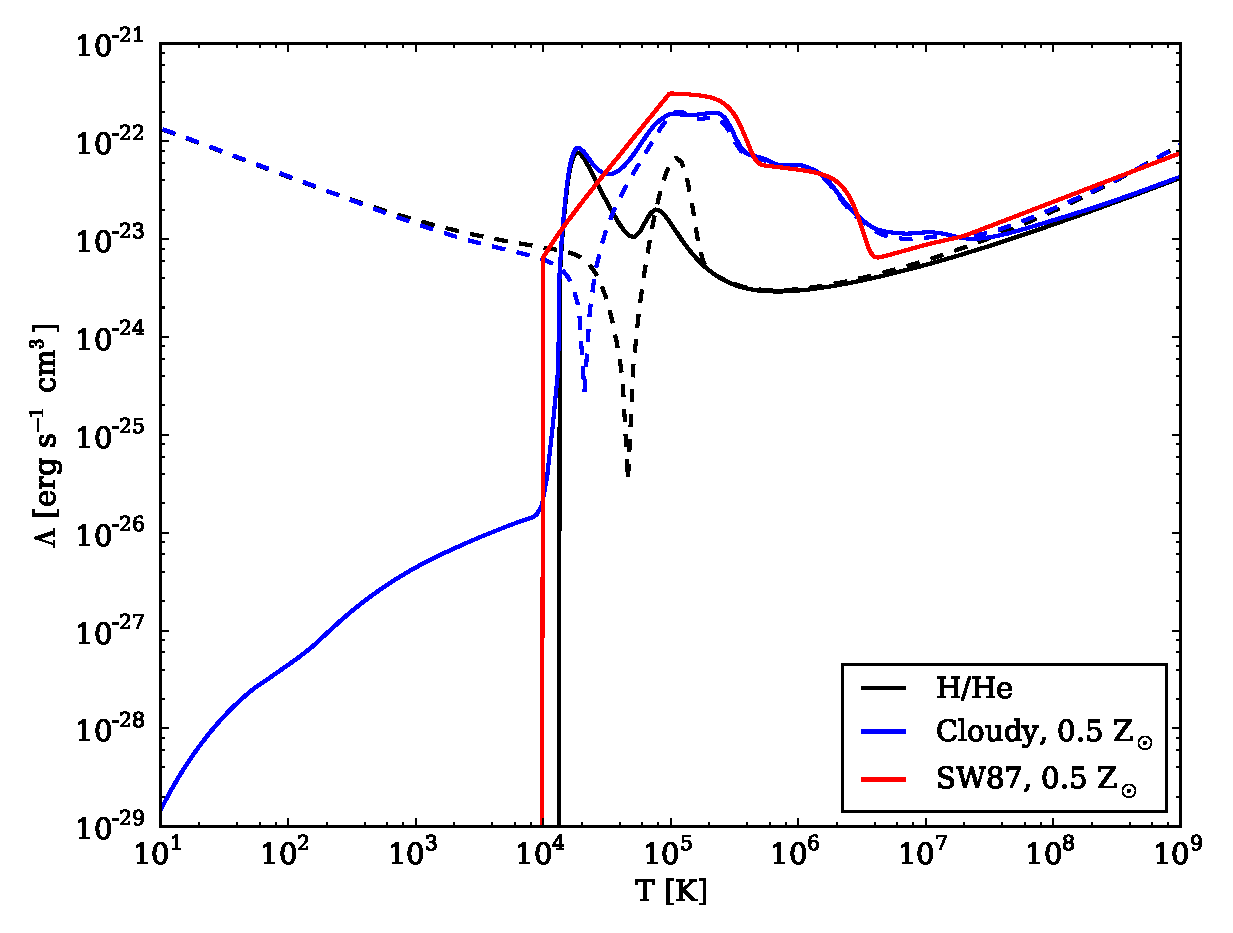
\includegraphics[width=1.0\textwidth]{figures/cooling_rate.eps}
  \end{center}
  \caption{Radiative cooling rates from the various cooling methods
    available in \enzo.  The black curves show cooling rates from a gas
    with primordial composition using the non-equilibrium chemistry
    network.  The blue curves are for a gas with metallicity of 0.5
    $Z_{\odot}$ computed with the Cloudy cooling method.  The solid
    black and blue lines assume collisional processes only while the
    dashed lines include photo-ionization and photo-heating from a UV
    metagalactic background at $z = 0$ with a gas number density of
    10$^{-4}$ cm$^{-3}$.  The rates shown by the
    dashed lines indicate a net heating below $T \sim 10^{4.5}$, where
    the rapid change in rate is evident (the curve is an absolute
    value so it can be shown on a log plot).  The red curve is the
    tabulated cooling function of \citet{SW87}, which assumes a fully
    ionized gas with metallicity of 0.5 $Z_{\odot}$.}
  \label{fig.cooling_rate}
\end{figure}
 

\section{Radiation}
\label{sec.allrad}
\subsection{Homogeneous radiation background}
\label{sec.num.rad-homogeneous}

Enzo supports the use of a set of spatially uniform (but possibly time-varying) radiation fields that can interface with the chemistry and cooling/heating routines described elsewhere.  Many of these use fits to the H, He and He$^+$ ionizing and photo-ionization heating rates that are of the form
\begin{equation}
\rm{rate} = k_0 * (1+z)^{\alpha} * \exp{\left( \frac{\beta *(z-z_0)^2 }{1 + \gamma * (z+z_1)^2} \right)}
\label{eq:homo_rad_template}
\end{equation}
where the constant coefficients $\alpha$, $\beta$, $\gamma$, $z_0$ and $z_1$ are fits from the literature.  


\begin{table}
\begin{center}
\caption{Homogeneous radiation field coefficients}
\begin{tabular}{lrrrrrr}
\tableline\tableline
{Element} & {$k_0$} &  {$\alpha$} & {$\beta$} & {$\gamma$} & {$z_0$} & {$z_1$}  \\
\tableline
\multicolumn{7}{c}{Radiation Type 1 \citep{1996ApJ...461...20H} for case $\alpha_q = 1.5$} \\
\tableline
H ionization & $6.7 \times 10^{-13}$ & 0.43 & 1/1.95 & 0 & 2.3 & 0 \\
He ionization & $6.3 \times 10^{-15}$ & 0.51 & 1/2.35 & 0 & 2.3 & 0 \\
He$^+$ ionization & $3.2 \times 10^{-13}$ & 0.50 & 1/2.00 & 0 & 2.3 & 0 \\
H heating & $4.7 \times 10^{-24}$ & 0.43 & 1/1.95 & 0 & 2.3 & 0 \\
He heating & $8.2 \times 10^{-24}$ & 0.50 & 1/2.00 & 0 & 2.3 & 0 \\
He$^+$ heating & $1.6 \times 10^{-25}$ & 0.51 & 1/2.35 & 0 & 2.3 & 0 \\
\tableline
\multicolumn{7}{c}{Radiation Type 2 \citep{1996ApJ...461...20H} for case $\alpha_q = 1.8$} \\
\tableline
H ionization & $5.6 \times 10^{-13}$ & 0.43 & 1/1.95 & 0 & 2.3 & 0 \\
He ionization & $3.2 \times 10^{-15}$ & 0.30 & 1/2.60 & 0 & 2.3 & 0 \\
He$^+$ ionization & $4.8 \times 10^{-13}$ & 0.43 & 1/1.95 & 0 & 2.3 & 0 \\
H heating & $3.9 \times 10^{-24}$ & 0.43 & 1/1.95 & 0 & 2.3 & 0 \\
He heating & $6.4 \times 10^{-24}$ & 0.43 & 1/2.10 & 0 & 2.3 & 0 \\
He$^+$ heating & $8.7 \times 10^{-26}$ & 0.30 & 1/2.70 & 0 & 2.3 & 0 \\
\tableline
\multicolumn{7}{c}{Radiation Type 3 \citep{Kirkman05}} \\
\tableline
H ionization &        $1.04 \times 10^{-12}$ & 0.231 & -0.6818 & 0.1646 & 1.855 & 0.3097 \\
He ionization &       $1.84 \times 10^{-14}$ & -1.038 & -1.1640 & 0.1940 & 1.973 & -0.6561 \\
He$^+$ ionization & $5.79 \times 10^{-13}$ & 0.278 & -0.8260 & 0.1730 & 1.973 & 0.2880 \\
H heating &            $8.86 \times 10^{-25}$ & -0.0290 & -0.7055 & 0.1884 & 2.003 & 0.2888 \\
He heating &         $5.86 \times 10^{-24}$ & 0.1764 & -0.8029 & 0.1732 & 2.088 & 0.1362 \\
He$^+$ heating &   $2.17 \times 10^{-25}$ & -0.2196 & -1.070 & 0.2124 & 1.1782 & -0.9213 \\
\end{tabular}
%\tablecomments{}
\end{center}
\end{table} 
\subsection{Radiation transport: ray tracing}
\label{sec.num.raytracing}

Stars and black holes strongly affect their surroundings through radiation.
Radiation transport is a well-studied problem; however, its treatment in
multidimensional calculations is difficult because of the dependence on seven
variables -- three spatial, two angular, frequency, and time.  The non-local
nature of the thermal and hydrodynamical response to radiation sources further
adds to the difficulty.  Here we briefly describe \enzo's ray tracing
implementation \moray, which is presented in full detail in
\citet{Wise11_Moray} with seven code tests and six applications.

%The radiative transfer equation in comoving coordinates
%\citep{Gnedin97} reads
%%
%\begin{equation}
%  \label{eq:rteqn}
%  \frac{1}{c} \; \frac{\partial I_\nu}{\partial t} + 
%  \frac{\hat{n} \cdot \grad I_\nu}{\bar{a}} -
%  \frac{H}{c} \; \left( \nu \frac{\partial I_\nu}{\partial \nu} -
%  3 I_\nu \right) = -\kappa_\nu I_\nu + j_\nu .
%\end{equation}
%%
%Here $I_\nu \equiv I(\nu, \mathbf{x}, \Omega, t)$ is the radiation
%specific intensity in units of energy per time $t$ per solid angle per
%unit area per frequency $\nu$.  $H = \dot{a}/a$ is the Hubble
%constant, where $a$ is the scale factor.  $\bar{a} = a/a_{em}$ is the
%ratio of scale factors at the current time and time of emission.  The
%second term represents the propagation of radiation, where the factor
%$1/\bar{a}$ accounts for cosmic expansion.  The third term describes
%both the cosmological redshift and dilution of radiation.  On the
%right hand side, the first term considers the absorption coefficient
%$\kappa_\nu \equiv \kappa_\nu(\mathbf{x},\nu,t)$, and the second term
%$j_\nu \equiv j_\nu(\mathbf{x},\nu,t)$ is the emission coefficient
%that includes any point sources of radiation or diffuse radiation.
%GB: this was moved to the equations section.

We solve the radiative transfer equation in comoving coordinates (given by Equation~\ref{eq:rteqn}).
We can make some appropriate approximations to reduce the complexity
of this equation in order to include radiation transport
in numerical calculations.  Typically timesteps in dynamic
calculations are small enough so that $\Delta a/a \ll 1$, therefore
$a_{em}/a \approx 1$ in any given timestep, reducing the second term to
$\hat{n} \partial I_\nu/\partial \mathbf{x}$.  To determine the
importance of the third term, we evaluate the ratio of the third term
to the second term.  This is $HL/c$, where $L$ is the simulation box
length.  If this ratio is $\ll 1$, we can ignore the third term.  For
example at $z=5$, this ratio is 0.1 when $L = c/H(z=5)$ = 53 proper
Mpc.  In large boxes where the light crossing time is comparable to
the Hubble time, then it becomes important to consider cosmological
redshifting and dilution of the radiation.  Thus equation
(\ref{eq:rteqn}) reduces to the non-cosmological form in this local
approximation,
%
\begin{equation}
  \frac{1}{c} \frac{\partial I_\nu}{\partial t} + 
  \hat{n} \frac{\partial I_\nu}{\partial \mathbf{x}} =
  -\kappa_\nu I_\nu + j_\nu .
\end{equation}
%
We choose to represent the source term $j_\nu$ as point sources of
radiation (e.g. stars, quasars) that emit radial rays that are
propagated along the direction $\hat{n}$.

Ray tracing is an accurate method to propagate radiation from point
sources on a computational grid as long as there are a sufficient
number of rays passing through each cell.  Along a ray, the radiation
transfer equation reduces to
%
\begin{equation}
\label{eqn:rtray}
\frac{1}{c} \frac{\partial P}{\partial t} + \frac{\partial P}{\partial
  r} = -\kappa P,
\end{equation}
where $P$ is the photon number flux along the ray.  To sample the
radiation field at large radii, ray tracing requires at least $N_{ray}
= 4\pi R^2 / (\Delta x)^2$ rays to sample each cell with one ray,
where $R$ is the radius from the source to the cell and $\Delta x$ is
the cell width.  If one were to trace $N_{ray}$ rays out to $R$, the
cells at a smaller radius $r$ would be sampled by, on average,
$(r/R)^2$ rays, which is computationally wasteful because only a few
rays per cell  are required to provide an accurate calculation
of the radiation field (as we will show later).

We avoid this inefficiency by utilizing adaptive ray tracing
\citep{Abel02_RT}, which is based on Hierarchical Equal Area isoLatitude
Pixelation \citep[HEALPix;][]{HEALPix} and progressively splits rays when the sampling
becomes too coarse.  In this approach, the rays are
traced along normal directions of the centers of the HEALPix pixels that 
evenly divide a sphere into equal areas.  The rays are initialized at
each point source with the photon luminosity (photon s$^{-1}$) equally
spread across $N_{\rm pix} = 12 \times 4^l$ rays, where $l$ is the
initial HEALPix level.  We usually find $l$ = 0 or 1 is sufficient
because these coarse rays will usually be split before traversing
the first cell.

The rays are traced through the grid in a typical fashion
\citep[e.g.][]{Abel99_RT}, in which we calculate the next cell
boundary crossing.  The ray segment length crossing the cell is
%
\begin{equation}
  \label{eqn:trace}
  dr = R_0 - \min_{i=1 \rightarrow 3} \left[(x_{\rm cell,i} - x_{\rm src,i}) /
    \hat{n}_{\rm ray,i} \right],
\end{equation}
%
where $R_0$, $\hat{n}_{\rm ray}$, $x_{\rm cell,i}$, and $x_{\rm
  src,i}$ are the initial distance traveled by the ray, normal
direction of the ray, the next cell boundary crossing in the $i$-th
dimension, and the position of the point source that emitted the ray,
respectively.  However before the ray travels across the cell, we
evaluate the ratio of the face area $A_{\rm cell}$ of the current cell
and the solid angle $\Omega_{\rm ray}$ of the ray,
%
\begin{equation}
  \label{eqn:split}
  \Phi_c = \frac{A_{\rm cell}} {\Omega_{\rm ray}} = 
  \frac{N_{\rm pix} (\Delta x)^2} {4\pi R_0^2}.
\end{equation}
%
If $\Phi_c$ is less than a pre-determined value (usually $>3$), the
ray is split into 4 child rays.  The pixel numbers of the child rays
$p^\prime$ are given by the ``nested'' scheme of HEALPix at the next
level, i.e. $p^\prime = 4 \times p + [0,1,2,3]$, where $p$ is the
original pixel number.  The child rays (1) acquire the new normal
vectors of the pixels, (2) retain the same radius of the parent ray,
and (3) get a quarter of the photon flux of the parent ray.
Afterward, the parent ray is discontinued.

A ray propagates and splits until at least one of the following conditions is met: (1) the photon has traveled $c
\times dt_P$, where $dt_P$ is the radiative transfer timestep; (2) its
photon flux is almost fully absorbed ($>99.9\%$) in a single cell,
which significantly reduces the computational time if the radiation
volume filling fraction is small; (3) the photon leaves the
computational domain with isolated boundary conditions; or (4) the
photon travels $\sqrt{3}$ of the simulation box length with periodic
boundary conditions.
In the first case, the photon is halted at that position and saved,
where it will be considered in the solution of $I_\nu$ at the next
timestep.  In the next timestep, the photon will encounter a different
hydrodynamical and ionization state, hence $\kappa$, in its path.
Furthermore any time variations of the luminosities will be retained
in the radiation field.  This is how this method retains the time
derivative of the radiative transfer equation.  The last restriction
prevents our method from considering sources external to the
computational domain. However, a uniform radiation background can be used
in conjunction with ray tracing that adds the background intensity to the
local radiation field. 

The radiation field is calculated by integrating Equation
(\ref{eqn:rtray}) along each ray, which is done by considering the
discretization of the ray into segments.  In the following
description, we assume the rays are monochromatic for simplicity.  For
convenience, we express the integration in terms of optical depth
$\tau = \int \kappa(r,t) \; dr$, and for a ray segment
%
\begin{equation}
  \label{eqn:dtau}
  d\tau = \sigma_{\rm abs}(\nu) n_{\rm abs} dr.
\end{equation}
Here $\sigma_{\rm abs}$ and $n_{\rm abs}$ are the cross section and
number density of the absorbing medium, respectively.  In the static
case, equation (\ref{eqn:rtray}) has a simple exponential analytic
solution, and the photon flux of a ray is reduced by
%
\begin{equation}
  \label{eqn:flux}
  dP = P \times (1 - e^{-\tau})
\end{equation}
as it crosses a cell.  We equate the photo-ionization rate to the
absorption rate, resulting in photon conservation \citep{Abel99_RT,
  Mellema06}.  Thus the photo-ionization and
photo-heating rates associated with a single ray ($k_{\rm ph}$ and
$\Gamma_{\rm ph}$, respectively)  are
%
\begin{equation}
  \label{eqn:kph}
  k_{\rm ph} = \frac{P (1 - e^{-\tau})}{n_{\rm abs} \; V_{\rm cell} \; dt_P},
\end{equation}
\begin{equation}
  \label{eqn:gamma}
  \Gamma_{\rm ph} = k_{\rm ph} \; (E_{\rm ph} - E_i),
\end{equation}
where $V_{\rm cell}$ is the cell volume, $E_{\rm ph}$ is the photon
energy, and $E_i$ is the ionization energy of the absorbing material.
In each cell, the photo-ionization and photo-heating rates from each
ray in the calculation are summed. After the ray tracing is
complete, these rates are used as inputs to the solver described in
Section~\ref{sec.ov.chem} to update the ionization, chemical, and energy states
of the gas in each cell.

%%% Local Variables: 
%%% mode: latex
%%% TeX-master: "ms"
%%% End: 
 
\subsection{Radiation transport: Flux-limited diffusion}
\label{sec.num.rad-fld}

%% With regards to the numerical method section, we're really looking for
%% something that's no more than a page long: a few relevant equations,
%% maybe a finite difference equation or two if you feel that it's
%% relevant, but primarily a description of the algorithms used for the
%% FLD solve and a brief explanation of how it's coupled to the
%% chemistry, as well as references to the relevant method paper(s).
%% Working in a reference or two to science papers is also great! 

In addition to the ray-tracing approach for radiation transport
described in Section~\ref{sec.num.raytracing}, \enzo\ currently includes
a field-based radiation transport solver for problems posed on uniform
(i.e.~non-AMR, non-SMR) grids, which has been tuned for large-scale simulations
involving many ionizing sources.  Detailed explanations of the model and
solution approach may be found in
\cite{NBHBROW2007}, \cite{ReynoldsHayesPaschosNorman2009} and
\cite{NRS2009}, the salient features of which are reproduced here. 
In addition, comparisons of this solver with other astrophysical
radiation transport solvers may be found in \cite{IlievEtAl2009}.  

\enzo's field-based radiation solver focuses on
a flux-limited diffusion approximation for cosmological radiative
transfer, with couplings to both the gas energy and chemical number
densities.
%\begin{eqnarray}
%  \label{eq:fld_radiation}
%  \partial_t E_r + \frac1a \div \left(E_r \vec{v}_b\right) &=& 
%    \div\left(D\grad E_r\right) -
%    \frac{\dot{a}}{a} E_r - c\kappa E_r + \eta, \\
%  \label{eq:fld_heating}
%  \partial_t e_c &=& -\frac{2\dot{a}}{a} e_c + G - \Lambda, \\
%  \label{eq:fld_chemistry}
%  \partial_t {\mathrm n}_i + 
%    \frac1a \div\left({\mathrm n}_i \vec{v}_b\right) &=& 
%    \alpha_{i,j} {\mathrm n}_e {\mathrm n}_j - {\mathrm n}_i
%    \Gamma_i^{ph}, \quad i=1,\ldots,N_s,
%\end{eqnarray}
%where $E_r$ is a grey radiation energy density, $e_c$ is the
%internal energy correction due to photo-heating and chemical cooling,
%and ${\mathrm n}_i$ correspond to the chemical number densities of
%HI, HII, HeI, HeII and HeIII, and ${\mathrm n}_e$ is the electron
%number density.  Here, we define the grey radiation energy density
%through first assuming a fixed frequency spectrum, i.e.
%$E_{\nu}(\nu,\vec{x},t) = \tilde{E}_r(\vec{x},t) \chi(\nu)$, and then
%defining the integrated quantity
%\begin{equation}
%\label{eq:grey_radiation_energy}
%   E_r(\vec{x},t) \equiv \int_{\nu_0}^{\infty}
%   E_{\nu}(\nu,\vec{x},t)\,\mathrm d\nu \  = \ 
%   \tilde{E}_r(\vec{x},t) \int_{\nu_0}^{\infty} \chi(\nu)\,\mathrm d\nu.
%\end{equation}
%In addition, $D$ in (\ref{eq:fld_radiation}) is the {\em Larsen
%square-root flux-limiter} (see \cite{Morel2000}), $\kappa$ is the total
%opacity, $\eta$ is the field of radiation sources, $G$ provides the
%radiation induced photo-heating, $\Lambda$ provides the chemical
%cooling, $\alpha_{i,j}$ are the reaction rate coefficients defining
%the interactions between species ${\mathrm n}_i$ and ${\mathrm n}_j$,
%and $\Gamma_i^{ph}$ are the radiation induced photo-ionization rates. 

The system of equations
(\ref{eq:fld_radiation}-\ref{eq:fld_heating}) along with the chemical network 
(Equation~\ref{eq:species_evolution}) is solved
independently of \enzo's hydrodynamics, gravity and dark-matter solvers
(Sections \ref{sec.hydro.ppm}-\ref{sec.ov.nbody}), thereby allowing
the advective portions of Equations (\ref{eq:fld_radiation}) and
(\ref{eq:species_evolution}) to be taken care of by the fluid solvers.
Due to the disparate time scales between radiation transport and chemical
ionization and heating, the remainder of these equations is solved
using an operator-split algorithm.  Within a given time step to evolve
$(E_r^n, e_c^n, {\mathrm n}_i^n) \to (E_r^{n+1}, e_c^{n+1}, {\mathrm
n}_i^{n+1})$, we first evolve equation (\ref{eq:fld_radiation}):
$(E_r^n, e_c^n, {\mathrm n}_i^n) \to (E_r^{n+1}, e_c^{n}, {\mathrm
  n}_i^{n})$.  This uses an implicit Euler time discretization, and a
second-order centered finite-difference spatial discretization,
resulting in a large linear system of equations.  These are solved
using a preconditioned conjugate gradient iteration, where the
preconditioner consists of a geometric multigrid solver.  Both of
these linear solvers are provided by the HYPRE linear solver library
(see \cite{FalgoutYang2002} and \cite{hypre-manual}). 

We then evolve the heating and chemistry system, Equations~(\ref{eq:fld_heating})
and (\ref{eq:species_evolution}):  
$(E_r^{n+1}, e_c^n, {\mathrm n}_i^n) \to (E_r^{n+1}, e_c^{n+1},
{\mathrm n}_i^{n+1})$.  Due to the lack of spatial derivatives (since
advection is handled elsewhere), this system is a coupled system of
nonlinear ordinary differential equations.  This utilizes an implicit
quasi-steady-state approximation, formulated as follows.  We consider
the modified equations,
\begin{eqnarray}
  \label{eq:fld_heating_qss}
  \frac{\partial e_c}{\partial t} &=& -\frac{2\dot{a}}{a} e_c +
    \Gamma\left(\bar{E}_r,\bar{\mathrm n}_i\right) - 
    \Lambda\left(\bar{E}_r,\bar{\mathrm n}_i\right), \\
  \label{eq:fld_chemistry_qss}
  \frac{\partial {\mathrm n}_i}{\partial t} &=& k_{i,j}\left(\bar{e}_c\right)
    {\mathrm n}_e \bar{\mathrm n}_j - {\mathrm n}_i 
    \Gamma_i^{ph}\left(\bar{E}_r\right), \quad i=1,\ldots,N_s,
\end{eqnarray}
where we have defined the time-centered ``background'' states
$\bar{E}_r = \left(E_r^{n}+E_r^{n+1}\right)/2$, 
$\bar{\mathrm n}_i = \left({\mathrm n}_i^{n}+{\mathrm n}_i^{n+1}\right)/2$
and $\bar{e}_c = \left(e_c^{n}+e_c^{n+1}\right)/2$.  These equations
may each be solved analytically for their solution at the time
$t$, which we denote by
\begin{eqnarray}
  \label{eq:fld_heating_qss_sol}
  e_c(t) &=& \text{sol}_{e}\left(t,\bar{E}_r,\bar{\mathrm n}_i,e_c^n\right), \\
  \label{eq:fld_chemistry_qss_sol}
  {\mathrm n}_i(t) &=& \text{sol}_{\mathrm n_i}
  \left(t,\bar{E}_r,\bar{e_c},\mathrm n_i^n\right), \quad i=1,\ldots,N_s. 
\end{eqnarray}
We then define a nonlinear system of equations to compute the
time-evolved solutions $\left(E_r^{n+1}, e_c^{n+1}, 
{\mathrm n}_i^{n+1})\right)$ as
\begin{eqnarray}
  \label{eq:fld_heating_qss_fe}
  f_e(e_c^{n+1},{\mathrm n}_i^{n+1}) &\equiv& e_c^{n+1} -
    \text{sol}_{e}\left(t^{n+1},\bar{E}_r,\bar{\mathrm n}_i,e_c^n\right)
    = 0, \\
  \label{eq:fld_chemistry_qss_fn}
  f_{\mathrm n_i}(e_c^{n+1},{\mathrm n}_i^{n+1}) &\equiv& 
    {\mathrm n}_i(t) - \text{sol}_{\mathrm n_i}
    \left(t,\bar{E}_r,\bar{e_c},\mathrm n_i^n\right)=0, \quad
    i=1,\ldots,N_s.  
\end{eqnarray}
This system of $N_s+1$ nonlinear equations is solved using a damped
fixed point iteration, 
\[
   U_i = U_i - \lambda f_i(U), \quad i=1,\ldots,N_s+1,
\]
where $U$ is a vector containing the solutions to equations
(\ref{eq:fld_heating_qss_fe}-\ref{eq:fld_chemistry_qss_fn}).  In this
iteration, for the first 50 sweeps we use $\lambda=1$, and for more
challenging problems if that does not suffice we switch to a damping
parameter of $\lambda=0.1$.
 

\section{Other physics}
\label{sec.otherphys}
\subsection{Thermal conduction}
\label{sec.num.conductions}

\enzo\ implements the equations of isotropic heat conduction in a manner
similar to that of \citet{2007ApJ...664..135P}, where we model the
flux of isotropic heat transport:

\begin{equation}
\mathbb{F} = -\kappa_{sp} \nabla T
\end{equation}

Where $\kappa_{sp}$ is the Spitzer conduction coefficient, $4.6 \times 10^{-7}$~T$^{5/2}$ erg
s$^{-1}$~cm$^{-1}$~K$^{-1}$ \citep{1962pfig.book.....S}, and using a
value for the Coulomb logarithm, $\log \Lambda = 37.8$, that is
appropriate for the intracluster medium \citep{1988xrec.book.....S}.
It is quite possible that the local heat flux can become unphysical in
the high-temperature, low-density cluster regime when using this
formulation; thus, we take into account the saturation of the heat
flux at a maximum level of

\begin{equation}
j_{sat} \simeq 0.4 n_e k_b T \left( \frac{2 k_b T}{\pi m_e} \right)^{1/2}
\end{equation}

\citep{1977ApJ...211..135C}, and to ensure a smooth transition between
the Spitzer regime and the saturated regime we define an effective
conductivity using the formalism of \citet{1988xrec.book.....S}

\begin{equation}
\kappa_{eff} = \frac{\kappa_{sp}}{1 + 4.2 \lambda_e / \ell_T} \; ,
\end{equation}

where $\lambda_e$ is the electron mean free path and $\ell_T \equiv T
/ |\nabla T|$ is the characteristic length scale of the local
temperature gradient.  Furthermore, it is important to note that the
overall level of thermal conductivity can be strongly affected
by the presence of magnetic fields, which may strongly suppress heat
flow.  The strength and distribution of magnetic fields in the
intracluster medium is poorly understood, and it is unclear to what
extent these magnetic fields will suppress conduction.  For the
purposes of the work described in this paper, we assume that the
conductivity of the plasma can be described in terms of an effective
conductivity, which can be expressed as a fraction f$_{Sp}$ of the
Spitzer conductivity (where f$_{Sp} \leq 1.0$ are considered physical
values).

Thermal conduction in a
plasma can be strongly affected by the presence of magnetic field
lines, which may strongly suppress heat flow perpendicular to the
magnetic field.  In that case, we allow for heat transport only
parallel to
the magnetic field lines in magnetohydrodynamic simulations.
Mathematically, this is treated as:

\begin{equation}
\mathbb{F} = -\kappa_{sp} \hat{b} (\hat{b} \cdot \nabla T)
\end{equation}

Where $\hat{b}$ is the unit vector denoting the direction of the
magnetic field.  As with the isotropic thermal conduction, we allow a
multiplicative factor f$_{Sp}$ to take into account the possible
behavior of magnetic fields below the resolution limit of the
simulation.

Both isotropic and anisotropic thermal conduction in \enzo\ are treated
in an operator-split manner.  Furthermore, within the heat transport
module, transport along the x, y, and z directions are computed in a
directionally-split fashion, with heat flux along each direction
calculated at the + and - faces of the cell using the arithmetic mean
of the cell-centered temperature in cells $n$ and $n+1$ or $n-1$ and
$n$, respectively (empirically, this is more stable than taking the
geometric mean of the cell-centered temperatures).  The addition of
transport along magnetic field lines requires the calculation of
cross-terms in the temperature derivatives at cell faces, which can
result in spurious oscillations in the temperature field in regions
where the temperature gradient is strong in more than one spatial
direction.  Controlling these oscillations requires the addition of a
flux limiter for calculations of the temperature field.  In this case,
we choose the monotonized central difference flux limiter
\citep{1977JCoPh..23..263V}, which serves to maintain numerical
stability without sacrificing substantial speed or accuracy.
 
\subsection{Star formation and feedback}
\label{sec.ov.star}

% \red{( (BWO) I am a little worried that this section is too
%   long. The editorial hatchet may be called for, but I think somebody
%   else (who didn't write the section in the first place) needs to
%   think it through. )}

\subsubsection{Overview}
% Overview of methodology

% \red{(BWO: can this whole paragraph go?)}
% While the physics discussed in other sections of this paper is crucial
% to the study of cosmological structure formation, most observations of
% galaxies in the infrared, optical, and ultraviolet wavelengths are of
% stellar populations.  Furthermore, stars eject energy and metal-
% enriched gas throughout their lives, drastically modifying their own
% environments' cooling properties.  Broadly speaking, the formation of
% galaxies and galaxy clusters cannot be completely modeled without
% including the feedback of energy and metals from stellar populations.
% In particular, it is thought that feedback is crucial for suppressing
% the large numbers of dwarf-like galaxies that CDM theories predict
% \citep{1991ApJ...381...14L,1991ApJ...379...52W}.  An early burst of
% star formation could remove a large fraction of cold gas from such
% systems \citep{1978MNRAS.183..341W,1991ApJ...367...45C}.  Also, the
% unexpectedly low luminosities of small clusters and groups (relative
% to the richest clusters) is commonly explained through feedback
% \citep{1991ApJ...383..104K}.  Energy ejected during the formation of
% the cluster ellipticals lowers the central density and hence the X-ray
% luminosity of such clusters \citep{1997ApJ...484L..21C}.  For all of
% these reasons, it is critical to include star formation and the
% feedback of energy and metals into the interstellar and intergalactic
% media in cosmological simulations.

% Modeling star formation in the context of galaxy formation forces one
% to confront two fundamental problems. The dynamical range required to
% study galaxy formation and evolution is substantial, and attempting to
% directly resolve the formation of individual stars in the context of a
% Milky Way-type galaxy is computationally unfeasible.  Also, a strong
% theoretical understanding of the details of star formation is
% currently lacking.  Due to these challenges, models of star formation
% in cosmological simulations are largely phenomenological, and the
% ``stars'' that are formed are in most cases meant to represent an
% ensemble stellar population (although not all; see
% Section~\ref{sec:starform_pop3}). 

Due to the computationally unfeasible number of stars in a galaxy
($10^{11}$) and the lack of detailed understanding of star formation, a
number of phenomenological star formation models are included in
\enzo.
%The \enzo\ code includes approximately ten models for star formation
%and feedback.  
Broadly speaking, these methods all work in similar
ways: at a specified time interval, all grid cells that are at the
highest local level of refinement (i.e., that have no child cells) are
examined to see if they meet a set of criteria for star formation.
This may simply be a baryon density threshold, but can also include more
complex tests, such as an examination of local cooling and dynamical
time scales, molecular hydrogen fraction, metallicity, and converging
gas flows.  If the star formation criteria are met, some mass of gas
is taken away from the cell in question and a ``star particle'' with
the same mass is placed in the center of that cell with the same
velocity as the removed gas.  This star particle is then
allowed to inject mass, momentum, thermal energy, metals, and possibly
magnetic fields and/or cosmic ray populations into its local
environment.  In general, the particle is treated as an ensemble of
stars, with feedback properties occuring over time according to the
assumed initial mass function of the stellar population.

In the following sections, we describe some of the more widely-used
star formation and feedback methods used in \enzo.  We note that
similar methods have been employed in many other codes used for galaxy
formation, with comparable implementations for both star formation and
feedback in other grid-based codes.  With regards to particle-based
codes, star formation is broadly similar in implementation, though
feedback is typically implemented in a very different way due to the
Lagrangian nature of the method \citep[see,
e.g.,][]{sh03a,sh03b,hs03}.

% Specific example: Cen & Ostriker
\subsubsection{Cen \& Ostriker}
\label{sec:starform_cen}

The Cen \& Ostriker method is a heuristic model of star formation on
galactic scales.  This method, first described by \citet{CO1992},
assumes that stars form in substantially overdense, converging, and
gravitationally unstable gas.  Algorithmically, each cell at the
locally highest level of refinement is examined at each timestep to
see if it meets the critiera for star formation.  Star particles
are allowed to form in a cell if the following criteria are met:
\begin{eqnarray}
\rho_b/\bar{\rho}_b & \geq & \eta,  \\[2mm]
\label{cendens}
%\end{equation} 
%\begin{equation}
\div \myvec{v}_b & < & 0, \\
\label{cencont}
%\end{equation}
%\begin{equation}
t_{\rm cool} & < & t_{\rm dyn} \equiv \sqrt{3 \pi / 32G \rho_{\rm tot}}, \\
%\end{equation}
%\begin{equation}
m_{b} & > & m_{J} \equiv G^{-3/2} \rho_{b}^{-1/2}c^{3} 
\left[ 1 + \frac{\delta\rho_{d}}{\delta\rho_{b}} \right]^{-3/2}
\end{eqnarray}
where 
%$\rho_b$ is the baryon density in that cell, $\bar{\rho_b}$ is
%the mean baryon density in the simulation, 
$\eta$ is the user-defined
overdensity threshold, 
%$\myvec{v}$ is the velocity of the gas in the
%cell, $\rho_{d}$ is the dark matter density, $\rho_{\rm tot} =
%\rho_{b} + \rho_{d}$, 
and $m_{b}$ and $m_{j}$ are the baryonic mass in the
cell and the Jeans mass of the cell, and c is the isothermal sound speed
in the cell.  If all of these criteria are met, the mass of a star
particle is calculated as \(m_{*} = m_{b} \frac{ \Delta t}{ t_{\rm
    dyn} } f_{\rm *eff} \), where $f_{\rm *eff}$ is the star formation
efficiency parameter.

If $m_{*}$ is greater than a minimum star mass $m_{\rm *min}$, a particle
is created and given several attributes: mass, a unique index number,
the time of formation $t_{\rm form}$, the local dynamical free-fall time
$t_{\rm dyn}$ and the metallicity fraction of the baryon gas in the cell
$f_{\rm Zb}$.  There is a user-defined minimum dynamical time
$T_{\rm dyn,min}$, which is observationally motivated and affects the
feedback rates (see below).  The particle is placed in the center of
the cell and given the same peculiar velocity as the gas in the cell,
and is then treated in the same manner as the dark matter particles.
An amount of gas corresponding to the new particle's mass is
removed from the cell.

% In addition, we have added a stochastic star formation algorithm that
% keeps track of all of the sub-mass threshold stars that should have
% been created and when the total mass of uncreated stars is greater
% than the minimum mass, a star particle is created.

% The feedback of energy and metals into the baryon gas is similar to
% the Kravtsov feedback, with some important differences.  

The star formation algorithm creates each star particle
instantaneously.  However, feedback should take place over a
significant timescale, as all of the stars contained within the ``star
particle'' would in reality form (and massive stars would die) over a
substantial period of time.  Therefore, we assume that for the
purposes of feedback that the mass of stars formed at a time $t$ with
timestep $\Delta t$ is:
\begin{equation}
\Delta m_{\rm sf} = \int_t^{t+\Delta t} \frac{dM}{dt} dt =
 \int_{\tau_0}^{\tau_1} m_* \tau e^{-\tau} d\tau =
 m_* \left[(1+\tau_0) e^{-\tau_0} - (1 + \tau_1) e^{-\tau_1} \right]
 \end{equation}
where $\tau_0 = (t-t_{\rm form})/t_{\rm dyn}$ and $\tau_1 = (t+\Delta t-t_{\rm form})/t_{\rm dyn}$.

%\begin{eqnarray}  
%\Delta m_{\rm sf} =  m_{*} \left[ \left(1 + \frac{t-t_{\rm
%        form}}{t_{\rm dyn}}  \right)
%%\nonumber \times \\ % uncomment for 2-column
%		   \exp{\left( \frac{-(t-t_{\rm form})}{t_{\rm dyn}} \right) }
%%                    \nonumber \\ 
%	       - \left( 1 + \frac{t+ \Delta t-t_{\rm form}}{t_{\rm dyn}} \right) 
%%	       \nonumber \\ 
%                    \exp{ \left( \frac{-(t+\Delta t-t_{\rm
%                            form})}{t_{\rm dyn}} \right)  }
%                   \right]
%\end{eqnarray}
%which can be represented more clearly in integral form:
%
%\begin{eqnarray}
%\int_{t}^{t+Dt} \frac{dM}{dt} dt = \int_{t}^{t+Dt} m_{*} 
%\frac{dt}{t_{\rm dyn}} \left( \frac{t-t_{\rm form}}{t_{\rm dyn}} \right) 
%%\nonumber \times \\ 
%\exp{ \left( - ~ \frac{t-t_{\rm form}}{t_{\rm dyn}} \right) }
%\end{eqnarray}

During this timestep, the star particle returns
metal-enriched gas and thermal energy from supernovae and from stellar
winds.  Since massive stars have very short lifetimes, we assume that
there is an immediate feedback of some fraction $f_{\rm SN}$ of the rest
energy from the stars into the gas, such
that $E_{\rm add} = f_{\rm SN} \Delta m_{\rm sf} c^2$, where c is the speed of
light.  In addition, a fraction $f_{Z*}$ of the stellar mass is fed back 
in the form of metals.  Finally, a fraction of the mass $f_{m*}$
is added back into the gas
along with momentum in order to simulate the mass ejection from
all stars (not just supernovae).

There are six user-defined parameters in this algorithm: three deal
with star formation ($\eta$, $m_{\rm *min}$ and $t_{\rm
  dyn,min}$), and three deal with feedback ($f_{\rm SN}$, $f_{Z*}$ and
$f_{m*}$).  Some of these parameters are completely free, while others
can be guided by observation or theory.  For example, the supernova
feedback parameter, $f_{\rm SN}$, can be constrained by assuming that, for
every $200 M_\odot$ of stars created, one supernova occurs, and this
event feeds back approximately $10^{51}$ ergs of thermal energy,
giving:

\begin{equation}
f_{\rm SN} = \frac{10^{51}\, \mathrm{erg}}{200~M_\odot\, c^2} \simeq 3 \times 10^{-6}
\end{equation}

The metal yield $f_{Z*}$, defined as the mass in metals produced per
unit mass of stars created, can be constrained by, e.g., the
theoretical model of \citet{1995ApJS..101..181W}.  This model suggests
that $f_{Z*} = 0.02$ is an appropriate number.  The minimum dynamical
time is set to be $t_{\rm dyn,min} = 10^7$~years to agree with the SN timescales
seen in nearby OB associations.

The other parameters, such as the overdensity threshold $\eta$,
minimum star mass $m_{\rm *min}$, and mass ejection fraction $f_{m*}$ are
not well constrained either theoretically or observationally.  Indeed,
$m_{\rm *min}$ is a purely numerical parameter designed to keep the code
from producing too many star particles, and thus has no observational
or theoretical counterpart.  The $\eta$ parameter, on the other hand,
nominally has physical meaning (i.e., the density above which star
formation must occur on a very short timescale in a self-gravitating
cloud); however, in the vast majority of simulations the densities
that are reachable are nowhere near the densities of protostellar
clouds, and thus this parameter becomes a rough proxy for finding the
densest environments in a given simulation.  
%Given the
%simulation-dependent nature of these parameters, it is critical to set
%them carefully, and with some sensitivity testing.

% Specific example: Kravtsov
\subsubsection{Schmidt-Law method}
\label{sec:starform_kravtsov}

This method of star particle creation is designed to reproduce
the global Schmidt law of star formation~\citep{2003ApJ...590L...1K,
  1959ApJ...129..243S}.  This algorithm is deliberately minimal, and
is explicitly geared towards modeling star formation in a
phenomenological way on kiloparsec scales.  Stars are assumed to form
with a characteristic gas timescale $\tau_*$ such that $\dot{\rho}_* =
\rho_{\rm gas}/\tau_*$. 
%where $\rho_{\rm gas}$ and $\rho_*$ are the
%baryon gas and stellar densities, respectively.  
This ``constant
efficiency'' model on the scale of star formation regions is well
motivated observationally
\citep{1996AJ....112.1903Y,2002ApJ...569..157W}.  Star formation is
only allowed to take place in very dense regions with $\rho_{\rm gas}
\geq \rho_{\rm SF}$, where $\rho_{\rm SF}$ is a constant proper (as
opposed to comoving) density threshold.  No other criteria are
imposed.  Typical choices for $\tau_*$ and $\rho_{\rm SF}$ are $\tau_*
= 4$ Gyr and $\rho_{\rm SF} = 1.64~$M$_\odot$~pc$^{-3}$~$(n_{\rm H}
\sim 50$~cm$^{-3})$.  The adopted timescale is derived from the
observationally-determined normalization of the Schmidt law, and the
density threshold is determined by observations of star forming
regions on $\sim 100$ pc scales.

Algorithmically, the star formation events in the Schmidt-law algorithm are
assumed to occur once every global timestep (with the constraint $\Delta t_0 \leq
10^7$ years).
In cells where star formation is determined to occur (i.e. $\rho_{\rm
  gas} \geq \rho_{\rm SF}$), star particles with a mass of $m_* =
\dot{\rho}_* V_{\rm cell} \Delta t_0$ (where $V_{\rm cell}$ is the
volume of the mesh cell) are assumed to form instantaneously in a
manner similar to that described in Section~\ref{sec:starform_cen}.
The \enzo\ implementation of this algorithm is similar, except that
instead of forming stars only at the root grid timestep, we allow
stars to form at the timestep of the highest level of resolution at
any particular point in space.  As can be seen from the equation for
$m_*$ above, this can result in very small stellar masses.  To avoid
memory and processor time issues related to having very large numbers
of star particles we impose a threshold mass $M_{\rm *,min}$ such that
a star particle only forms if $m_* \geq M_{\rm *,min}$.  An
appropriate choice of $M_{\rm *,min}$ does not significantly change
the star overall star formation history of a simulation, though it may
delay the onset of star formation in a given cell relative to a
simulation without a particle mass threshold.

Each ``star particle'' is assumed to represent an ensemble of stars
and is treated as a single-age stellar population (as in the previous
section).  Kravtsov assumes that the stellar initial mass function (IMF) is described by a Miller \&
Scalo functional form with stellar masses between $0.1$ and
$100~M_\odot$ \citep{1979ApJS...41..513M}.  All stars in this IMF with
$M_* > 8~M_\odot$ deposit $2 \times 10^{51}$ erg of thermal energy
and a mass $f_z M_*$ of metals into the cell in which they form
without delay, with $f_z \equiv \min(0.2, 0.01~M_*-0.06)$
(i.e. instantaneous deposition of metals).  The definition of $f_z$ is
a rough approximation of the results of \citet{1995ApJS..101..181W}.

% Kravtsov reports that simulations with this algorithm reliably
% reproduce the star formation rate-gas surface density relation of the
% Schmidt law, and are not particularly sensitive to numerical
% parameters \citep{2003ApJ...590L...1K}.  He also notes that this
% algorithm is surprisingly insensitive to the presence or absence of
% feedback and details of the cooling and heating properties of the gas,
% which suggests that the global star formation rate is determined by
% gravitationally- driven supersonic turbulence (on large scales) rather
% than stellar feedback or thermal instabilities on small scales.

% Specific example: H2-regulated
\subsubsection{\HH-regulated method}
\label{sec:starform_H2reg}

The methods described in the previous two sections are generally used
in simulations that have relatively poor resolution, $\Delta x \ga 1$~kpc.
At this physical scale, individual star forming regions are not
resolved, so all uncertainty about the behavior of molecular clouds is
folded into a density threshold for star formation.  In calculations
with much higher resolution, however (on the order of a few pc), individual
molecular clouds can be resolved, thus rendering these approximations
invalid.  To that end, \citet{2012ApJ...749...36K} have implemented
a star formation algorithm that is specifically geared to
high-resolution cosmological simulations of galaxy formation, where
the formation of molecular hydrogen is followed directly and stars
are allowed to form at the highest level of refinement when the local
H$_2$ fraction exceeds a pre-determined threshold.  Cells are examined
every root grid timestep, $\Delta t_0$, and cells at the highest level
that exceed the H$_2$ limit form star particles with masses
proportional to the inferred mass of molecular hydrogen in the
star-forming region
\citep{2008ApJ...689..865K,2009ApJ...693..216K,2010ApJ...709..308M}.
The mass of the particle is calculated as:
\begin{equation} 
m_p = \epsilon \rho_{\rm gas} (\Delta x_{m})^3 \frac{\Delta t_0}{t_*}
\end{equation}
where $\Delta x_{m}$ is the resolution of the maximum level of
refinement, $\epsilon$ is an efficiency parameter with a standard
value of 0.01 \citep[as motivated by][]{2007ApJ...654..304K}, and
t$_*$ is the local free-fall timescale.

The feedback method used in this method is identical to that described
in Section~\ref{sec:starform_cen}.

% Specific example: Pop III
\subsubsection{Population III star formation}
\label{sec:starform_pop3}

Unlike in the previous sections, under some circumstances it is both
possible and desirable to simulate stars individually, rather than
treating particles as ensembles.  One particular example of this is
Population III star formation
\citep{ABN02,2007ApJ...654...66O,2008ApJ...685...40W,2009Sci...325..601T},
where a given halo may only form one star of primordial composition.
To accommodate this, \enzo\ contains a star formation algorithm that
forms individual Population III stars directly \citep{2007ApJ...659L..87A,
  2008ApJ...685...40W, 2012MNRAS.427..311W}.  Using criteria similar
to~\citet{CO1992}, a star particle forms when a cell meets all of the
following conditions:

\begin{enumerate}
\item A baryon overdensity of $5 \times 10^5$ (corresponding to a
  hydrogen number density of 
  roughly $10^3$ cm$^{-3}$ at $z=10$),

\item A converging gas flow ($\div \myvec{v} < 0$), and

\item A molecular hydrogen mass fraction f$_{\rm H2} > 5 \times 10^{-4}$,
\end{enumerate}

These are comparable to the conditions typical of a collapsing metal-free molecular cloud roughly
10 million years before the birth of a Pop III main-sequence star.  If
multiple neighboring cells are flagged as being able to form stars, a
single star is created instead.  This star has a mass that is randomly
sampled from a stellar IMF with a functional form of

\begin{equation}
f(\log M) dM = M^{\alpha} \exp \Big[ -\Big( \frac{M_{\rm char}}{M}
\Big)^{\beta} \Big]
\end{equation}

Feedback from Population III stars created using this algorithm comes in multiple forms.
Radiative feedback using the Moray radiation transport algorithm
\citep{Wise11_Moray} is available, using the mass-dependent hydrogen
ionizing and Lyman-Werner photon luminosities and lifetimes of the
Population III stars from \citet{2002A&A...382...28S}.  At the end of
their main-sequence lifetimes, explosion energies, ejected gas mass,
and ejected metal are calculated using a variety of sources that
depend on the mass of the star, and are described in detail in Section
3.2.1 of \citet{2012MNRAS.427..311W}.


%%% Local Variables: 
%%% mode: latex
%%% TeX-master: "ms"
%%% End: 


% this is its own section
\subsection{Time Stepping}
\label{sec.timestepping}

%\dcc{Made this its own section (not really part of the AMR, it's more
%  general than that.)  Added stuff on harmonic average for 3d. See
%  note below on acceleration timestep criterion being crap. Moved
%  w-cycle to the previous section}

In \enzo, resolution of the equations being solved is adaptive in time 
as well as in space.  The timestep in \enzo\ is satisfied on a level-by-level
 basis by finding the largest timestep such that multiple criteria are
satisfied on each level.  The timestep criteria used by Enzo are 
(showing the one-dimensional case for clarity):

\begin{equation}
\Delta t_{hydro} = min \left( \kappa_{hydro} \frac{a \Delta x}{c_{s} + |v_x|} \right)_L ,
\label{eqn:dthydro}
\end{equation}

\begin{equation}
\Delta t_{dm} = min \left(\kappa_{dm} \frac{a \Delta x}{v_{dm,x}} \right)_L ,
\label{eqn:dtdarkmatter}
\end{equation}

\begin{equation}
\Delta t_{exp} = f_{exp} \left( \frac{a}{\dot{a}} \right) ,
\label{eqn:dtexpand}
\end{equation}

\begin{equation}
\Delta t_{accel} = min \left( \sqrt{\frac{\Delta x}{\vec{g}}} \right)_L 
\label{eqn:dtaccel}
\end{equation}

 In equations~\ref{eqn:dthydro}-\ref{eqn:dtaccel}, the $min ( \ldots )_L$
formalism means that this value is calculated for all cells on a given level
L and the minimum overall value is taken as the timestep.  
Equation~\ref{eqn:dthydro} ensures that all cells satisfy the 
Courant-Freidrichs-Levy (CFL) condition for accuracy and stability of an explicit
finite difference discretization of the Euler equations.  Effectively this condition
forces the timestep to be small enough such that any changes in the fluid propagate
less than a single grid spacing, $\Delta x$.  In this equation, $\kappa_{hydro}$ is 
a numerical constant with a value of $0 < \kappa_{hydro} \leq 1$ (with a typical
value of $\kappa_{hydro} \sim 0.3-0.5$) that ensures that the CFL condition is always
met, and $c_s$ and $v_x$ are the sound speed and peculiar baryon
velocity in a given cell.

Equation~\ref{eqn:dtdarkmatter} is analogous to Equation~\ref{eqn:dthydro} and ensures
accuracy in the N-body solver by requiring that no dark matter particle travels more than
one cell width.  The parameter $\kappa_{dm}$ is analogous to $\kappa_{dthydro}$, with
an identical range of values.  Equation~\ref{eqn:dtexpand} limits the timestep such 
that the expansion parameter a can only change by a fractional amount of $f_{exp} = \Delta a/a$, 
where $f_{exp}$ is a user-defined parameter and has typical values of $f_{exp} = 0.01-0.02$.
This is required for the stability of the PPM algorithm in comoving coordinates, and
typically limits the timestep only at high redshifts when densities are relatively
homogeneous.

Equation~\ref{eqn:dtaccel} is supplementary to equation~\ref{eqn:dthydro} in that it
takes into account the possibility of large accelerations causing numerical 
instabilities by violating the Courant condition.  In this equation, $\vec{g}$ is the
gravitational acceleration in each cell on level L.  \blue{ \emph{It should be
  noted that the timestep is computed before the acceleration field is computed,
  and the acceleration field is deleted at the end of each time step.
  So this condition isn't ever actually enforced.  We should either
  fix this problem, or not discuss it.
 -dcollins.} }

Equation ~\ref{eqn:dthydro} is valid for one dimension.  For 2 or 3
dimensions, it was shown by \cite{Godunov1959}  that using the
harmonic average of the timestep found along each of the coordinate
axes yields a maximum $\kappa_{hydro} = 0.8$.  So letting $\Delta
t_x$, $\Delta t_y$, and $\Delta t_z$ be the analogues of
eqn. \ref{eqn:dthydro} along the $x,y$ and $z$ axes, 
\begin{equation}
\Delta t_{hydro} = min ( \kappa_{hydro} /( \frac{1}{\Delta t_x}
+\frac{1}{\Delta t_y} + \frac{1}{\Delta t_z} ) )_L
\end{equation}

For all other criteria, multiple dimensions are accounted for by
repeating the one dimensional criterion along each axis, and taking
the minimum.


% this is its own section
% EJT: general changes
% Enzo to \enzo\
% changed ``some Lagrangian fluid trajectories'' to ``a fixed number of Lagrangian fluid trajectories.'' Easier to understand.
% changed ``some evolution'' to ``a period of evolution'' ... I basically don't like 'some'. It sounds vague.
% rephrased to remove ``e.g.'' as they read slightly awkwardly
% moved definition of T_1 and T_2 slightly higher in shock text to where they first appear.

\section{Analysis}
\label{sec.num.analysis}

\subsection{Inline analysis with yt}

Detailed analysis of simulation results requires both the tools to ask
sophisticated questions of the data and the ability to process vast quantities of
data at high time-cadence.  As simulations grow in size and complexity, storing data
for post-processing simply becomes intractable.  To cope with this, we have
instrumented \enzo\ with the ability to conduct analysis during the course of a
simulation.  This enables analysis with extremely high time cadence (even as often
as every subcycle of the finest refinement level), without
attempting to write an entire checkpoint output to disk.  The current mechanism
for conducting analysis in \enzo\ during the course of the simulation utilizes
the same compute resources as used by the simulation itself by transferring their usage 
from \enzo\ to the analysis routines; this is often
referred to as \textit{in situ} analysis or visualization.  Utilizing a
dynamically-scheduled second set of computing resources, often referred to as
\textit{co-scheduled} analysis or visualization, provides greater flexibility and overall
throughput at the expense of simplicity.

We expose \enzo's mesh geometry and fluid quantities to the analysis platform
\texttt{yt} \citep{2011ApJS..192....9T, 2011arXiv1112.4482T}.  At compile time,
\enzo\ is (dynamically or statically) linked against the Python and NumPy
libraries necessary to create proxy objects exposing the mesh geometry,
fluid quantities and particle arrays as NumPy arrays.  This information is then
passed to a special handler inside \texttt{yt}.  \texttt{yt} interprets the
mesh and fluid information and, without saving data to disk, constructs a native representation of the in-memory state
of the simulation that appears identical to an on-disk simulation output.
\enzo\ then executes a user-provided analysis script, which is able to access the
in-memory simulation object.  Once the analysis script has returned control to
\enzo, the simulation proceeds.  This process can occur at either the top of the
main ``EvolveHierarchy'' loop or at the end of a timestep at the finest level,
and the frequency with which it is called is adjustable by a run-time
parameter.  During the course of conducting analysis, the simulation is halted
until the conclusion of the analysis.

Most analysis operations that can be performed on data sets that reside on
disk can be performed on in-memory data sets in \texttt{yt}.  This includes
projections (i.e., line integrals, both on- and off-axis), slices, 1-, 2-, and
3-D fluid phase distributions, calculation of derived quantities and arbitrary
data selection.  As of version 2.5 of \texttt{yt},  the Rockstar phase-space
halo finder \citep{2013ApJ...762..109B} can be executed through \texttt{yt} on
in-memory \enzo\ data.  Operations that currently cannot be conducted on
in-memory datasets are those that require spatial decomposition of
data.  For 
instance, calculating marching cubes on a data object with \texttt{yt} is a
fully local operation and can be conducted \textit{in situ}.  However,
calculating topologically-connected sets requires a spatial decomposition of
data and thus cannot be conducted \textit{in situ}.  This prohibition extends
to halo finding operations other than Rockstar, most multi-level
parallelism operations, and volume rendering.

Where microphysical solvers or other operator-split physics calculations can be
done in Python, \texttt{yt} can serve as a driver for these calculations.  A
major feature set that is currently being developed is to pass structured
(i.e., non-fluid) information back from \texttt{yt} into \enzo.  For instance,
this could be the result of semi-analytic models of the growth and evolution of
star clusters, galaxy particle feedback parameters that have been influenced by
merger-tree analysis, or even spectral energy distributions that are calculated
within \texttt{yt} and provided to \enzo\ as input into radiative transfer
calculations.  Future versions will include this, as well as the ability to
dynamically allocate compute resources to \texttt{yt} such that the simulation
may proceed asynchronously with analysis (\textit{co-scheduled} analysis).
With this functionality will also come the ability to dynamically partition
data, such that spatially-decomposed operations such as volume rendering become
feasible during the course of a simulation.

\subsection{Tracer particles}

One of the inherent drawbacks of a grid-based fluid method is the
inability to follow the evolution of a single parcel of fluid as it
travels through the simulation volume.  To address this, \enzo\ has the
capability to introduce Lagrangian ``tracer particles'' into a
calculation either at the beginning of the simulation or when
restarting the calculation.  These tracer particles are put into the
simulation in a rectangular solid volume with uniform, user-specified
spacing.  Each particle's position and velocity is updated over the
course of a single timestep $\Delta t$ as follows:

\begin{eqnarray}
\label{eqn.drifttrace}
x^{n+1/2} & = & x^n + (\Delta t/2) v^{\rm interp,n} \nonumber \\
v^{n+1} & = & v^{\rm interp,n+1} \\
x^{n+1} & = & x^{n+1/2} + (\Delta t/2) v^{n+1} \nonumber
\end{eqnarray}

This is essentially a drift-kick-drift particle update from time $n$
to time $n+1$ -- however, instead of computing an acceleration at the
half-timestep $t^n + \Delta t/2$ (as is done for massive particles --
see Equation~\ref{eqn.driftkick}), the particle's velocity is updated
both at the beginning of each timestep and at the half-timestep
by linearly interpolating the cell-centered baryon velocity to the
position of the particle ($v^{\rm interp}$), and assigning it to that value.

\enzo saves tracer particle data at user-specified intervals,
independent of the intervals at which regular data sets are written.  The data written out
typically includes the tracer particle's unique ID, position, velocity, density,
and temperature, but is easily extensible to output any grid-based
quantity that a user requires.  This capability has been used quite
effectively in several papers, including \citet{2010ApJ...715.1575S}
and \citet{2012ApJ...748...12S}. It is crucial to keep in mind that
tracer particles model a fixed number of Lagrangian fluid trajectories. The fluid
on the grid, however, models the motion of all the mass and represents
the average quantity in a grid cell's volume. Consequently, after a period of
evolution, tracer particles --even if they initially had the same
density distribution as the gas-- will not have the same density
distribution as the fluid. For example, they tend to accumulate at stagnation points
of the flow, and care has to be taken in using these particles
appropriately. Tracer particles are very useful in studies such as the variety of
histories of the hydrodynamic quantities in Lagrangian fluid elements
and when evaluating complex chemical and cooling models in regard to the
simpler ones used in the actual numerical evolution.  

\subsection{Shock finding}

Identification of shocks and their pre- and post-shock conditions can be
accomplished through a combination of either temperature or velocity jumps with
dimensionally split or unsplit search methods.  The primary method used in
\enzo~is the dimensionally unsplit temperature jump method described in detail
in \citet{2008ApJ...689.1063S}.  We briefly outline the method here.

For every cell, we first determine whether it satisfies the following conditions
necessary to be flagged as a shock:

\begin{eqnarray}
\div \myvec{v} < 0,\\
\grad T \cdot \grad S > 0,\\
T_2 > T_1,\\
\rho_2 > \rho_1,
\end{eqnarray}

where $\myvec{v}$ is the velocity field, $T$ is the temperature, $\rho$ is the
density, and $S=T/\rho^{\gamma-1}$ is the entropy.  $T_2$ and $T_1$ are the post-shock~(downstream)
and pre-shock~(upstream) temperatures, respectively. An optional temperature floor
may be chosen, which is useful for situations such as cosmological simulations without a radiation
background where underdense gas in the intergalactic medium (IGM) can cool adiabatically to
very low temperatures.

Once a cell is flagged, the local temperature gradient is calculated, which is 
then used to traverse cells parallel to the gradient to search for the first
pre- and post-shock cell that do not satisfy the above conditions.  If during
the search a cell satisfying the conditions is found to have a more convergent
flow, that cell is marked as the center, and the search is started again. Using the 
temperature values from each of these cells, the Mach number is then solved
using the Rankine-Hugoniot temperature jump conditions:
\begin{equation}
\frac{T_2}{T_1} = \frac{(5\Mach^2 - 1)(\Mach^2 + 3)}{16\Mach^2},
\end{equation}
where $\Mach$ is the upstream Mach number.  

Shock finding in the context of AMR is applied grid-by-grid.  If a search for
pre/post-shock cells goes outside the bounds of the grid ghost zones, the
search is stopped for that particular shocked cell. In most situations this is
adequate since the hydrodynamic shock is captured in fewer than the number of
ghost zones.  Shock finding can be run either upon data output, or at each step
in the evolution of an AMR level if the Mach and pre/post-shock quantities are
needed for additional physics modules.



%% Section: code tests
%%  this should probably be done with one file per test

%%%%%%%%%%%%%%%%%%%%%%%%%%%%%%%%%%%%%%%%%%%%%%%%%%%%%%%%%%%%%%%%%%%%%%%%%%%%%
\section{Code tests}
\label{sec.tests}

Ensuring that a complex piece of software is behaving correctly is a
non-trivial task.  While there are a range of techniques that one can
apply to ensure correctness, the \enzo\ code uses two primary methods:
a suite of test problems that can be compared to previous versions of
the code, to ensure that \enzo\ is running correctly on a new
computer, with a new compiler, or after substantial changes have been
made to the code base; and by direct comparisons to other
astrophysical fluid dynamics codes.  We describe the \enzo\ test
methodology in Section~\ref{sec.tests.suite}, code comparisons in
Section~\ref{sec.tests.compare}, and show a small set of
representative test problems in Section~\ref{sec.tests.problems}.  We
further note that the \enzo\ test suite
(Section~\ref{sec.tests.suite}) contains hundreds of test problems, as
well as the ability to compare to a ``gold standard'' solution, and
thus all of the tests shown here are easily reproducible by the
reader.

%%%%%%%%%%%%%%%%%%%%%%%%%%%%%%%%%%%%%%%%%%%%%%%%%%%%%%%%%%%%%%%%%%%%%%%%%%%%%
\subsection{Verifying and validating the \enzo\ code}
\label{sec.tests.vandv}

\subsubsection{The \enzo\ test suite}
\label{sec.tests.suite}

\enzo\ is capable of simulating a large variety of problems types,
with all but a few of these types requiring only a parameter file as an
input.  The notable exception is the cosmology simulation, which takes
as input initial conditions created by other codes.  The suite of test
problems spans a wide range in complexity.  At one end of this spectrum
are simple problems that utilize only a single component of \enzo\ and
for which analytic solutions exist for comparison with the simulation
results.  At the opposite end are problems that exercise a large
portion of \enzo's machinery in concert.  Together, the available
problem types fully cover all of \enzo's functionality.  This enables
them to serve as a vehicle for verifying that the code's behavior
remains stable over time and after modifcation of the codebase.

\enzo\ uses an automated testing framework that allows a user to run,
with a single command, a set of test problems and compare the results
against results produced by any other version of the code.  Within the
\enzo\ source distribution, the test problem parameter files are stored
in a nested directory structure organized according to the primary
functionality tested, e.g., hydrodynamics, gravity, cooling, etc.
Each parameter file is accompanied by a text file containing various
descriptive keywords, such as the machinery tested, the
dimensionality, and the approximate run time.  A test runner script is
responsible for taking as input from the user a series of keywords
that are used to select a subset of all available test problems.  The
test problems are also grouped into three suites: the quick, push, and
full suites, each a superset of the ones named before.  The quick
suite is considered to minimally cover the primary functionality in
\enzo\ and is designed to be run repeatedly during the development
process.  The push suite has slightly increased feature coverage and
is mandated to be run before code changes are accepted into the main
repository.  The full suite consists of all test problems that can be
run with no additional input.  Approximate run times for the quick,
push, and full suite are 15 minutes, 1 hour, and 60 hours,
respectively, on a relatively new desktop computer (circa 2013).

After the test problems are selected by the test runner script, they
are run in succession using either the \enzo\ executable contained
within that distribution or an external executable built from another \enzo\
version and specified by the user.  This allows for any version of the
code to be tested with an identical set of test problems.  After
running the test problem simulations, the test runner then performs a
series of basic analysis tasks using the \texttt{yt} analysis toolkit
\citep{2011ApJS..192....9T, 2011arXiv1112.4482T}.  The default
analysis performed on all test problems includes calculation of
various statistics, such as extrema; mean; and variance, on the fields
present in the output data.  Custom analysis provided by scripts that
accompany the test problem parameter files is run for special cases,
such as when an analytical solution exists that can be compared
against the simulation data.  After the analysis is performed, the
results are compared against a set of gold standard results that are
maintained on a website and downloaded on the fly by the test runner
script.  Alternately, results from any version of \enzo\ can be stored
locally and compared to any other version of the code.  In
Section~\ref{sec.tests.problems}, we describe some of the key test
problems that are used to verify proper behavior.  All of these test
problems, as well as the scripts to generate the figures from them,
are available in the \enzo\ test suite, allowing the interested reader
to regenerate all of the figures in Section~\ref{sec.tests.compare}
using the \textit{'methodpaper'} suite of test problems.

\subsubsection{Code comparisons}
\label{sec.tests.compare}

Over the course of its existence, \enzo\ has been involved in numerous
comparisons with other astrophysical codes used for self-gravitating
fluid dynamics.  In general, \enzo\ behaves in a manner similar to other
grid-based (and particularly AMR-based) codes, as we will summarize below.

\enzo\ has been involved in multiple cosmological code comparisons,
including the Santa Barbara Cluster code comparison project
\citep{SantaBarbara}, a large comparison of N-body simulations
\citep{2008CS&D....1a5003H}, as well as several direct comparisons
between \enzo\ and the GADGET SPH code under a variety of
circumstances, including N-body and adiabatic hydrodynamics
\citep{2005ApJS..160....1O,2005MNRAS.364..909V, 2011MNRAS.418..960V}
and simulations of the Lyman-alpha forest \citep{2007MNRAS.374..196R}.
The \enzo\ code typically has a more difficult time resolving
small-scale self-gravitating structures (for an equivalent dark matter
particle count and nominally equivalent force resolution), but does
comparably well as a tree-based code for larger structure, and is
typically superior in terms of resolving fluid features due to its
higher-order (and artificial viscosity-free) Piecewise Parabolic
Method hydrodynamics solver.  When examining classical test cases such
as the Santa Barbara project \citep{SantaBarbara}, \enzo\ forms galaxy
clusters with very similar density, temperature, and entropy profiles
to other grid-based codes that use Godunov-type hydro methods, which
systematically differed from particle-based codes using SPH in this
code comparison.  Similarly, in galaxy cluster simulations that look
specifically at the properties of cosmological shocks
\citep[e.g.][]{2011MNRAS.418..960V}, \enzo\ produces results that are
similar to other high-order grid-based hydrodynamics codes, and far
superior performance of \enzo\ is observed (in terms of resolution of
fluid features and shock detection) in low-density regions when
compared to a particle-based code.  In tests of the Lyman-alpha forest
that include radiative cooling and a uniform metagalactic ultraviolet
background, \enzo\ and Gadget provide results on metrics such as the
matter power spectrum that are comparable to within 5\%
\citep{2007MNRAS.374..196R}.

Several comparisons have been made that focus specifically on
hydrodynamics solvers and fluid behavior.  In particular, the work of
\citet{2007MNRAS.380..963A} and \citet{Tasker2008} perform
head-to-head comparisons between several grid- and particle-based
codes for a variety of fluid-centric test problems (including shocked gas clouds,
self-gravitating, translating clouds, and Sedov-Taylor explosions),
and show that \enzo\ is comparable or superior in behavior to the
other grid-based hydrodynamics codes involved in the comparison, and
provide useful information on the sort of practical challenges that a
user of an
AMR code such as \enzo\ may experience.  More specific comparisons, including one
specifically testing the linear and nonlinear growth of the
Kelvin-Helmholz instability \citep{2012ApJS..201...18M}, as well as a
comparison that more
broadly examines Galilean invariance in grid-based codes
\citep{2010MNRAS.401.2463R}, show that \enzo, and in particular its
implementation of the Piecewise Parabolic Method hydrodynamics solver,
converge to the correct solution as expected, and generally provide
less diffusive solutions than lower-order codes, including those that
use artificial viscosity.  Finally, two code comparison projects have
been undertaken to examine turbulence in hydro codes -- one studied
the behavior of decaying isothermal supersonic turbulence
\citep{2009A&A...508..541K}, and the other looked at supersonic
magnetohydrodynamical turbulence \citep{2011ApJ...737...13K}.  Both
included the \enzo\ code, with the former testing the PPM
hydrodynamics and the latter the constrained transport MHD
implementation of \citet{Collins10}.  In both cases, \enzo\ performed similarly to other
grid-based codes that use Godunov-based fluid solvers, and typically
had better effective resolution than particle-based codes using the
same number of particles as the \enzo\ simulation used grid cells.

Three other comparisons between the \enzo\ code and other simulation
tools have been performed that focus on physics other than gravity and
fluid flow.  The flux-limited diffusion radiation transport scheme was
measured against several test problems by \citet{IlievEtAl2009},
producing results that are similar to both expected results (i.e.,
analytic test problems) and other methods (i.e., codes using other
methods, written by other groups), although there are some minor
differences (although all codes in the study exhibited differences
from the majority of other codes on at least a subset of the tests).
\citet{2011ApJ...726...55T} shows the results of varied reaction rate
coefficients for the formation of molecular hydrogen via the 3-body
process in both the \enzo\ and Gadget-2 codes.  Similar trends were
visible in both the \enzo\ and Gadget simulations, though at a
nominally equivalent resolution (i.e., with particle and cell gas
masses being comparable) \enzo\ simulations typically displayed a
substantially higher level of gas structure.  This is unsurprising due
to \enzo's higher-order hydro solver.  Finally,
\citet{2012ApJ...744...52P} show the results of comparing \enzo\ in
its non-AMR mode to a smoothed-particle hydrodynamics code, SNSPH, in
the context of common-envelope binary stellar interactions.  The
authors show that the codes display reasonable convergence properties
as a function of simulation resolution, and also agree quite well with
each other -- however, the observed mass-loss rates do not agree
particularly well with observations.

%%%%%%%%%%%%%%%%%%%%%%%%%%%%%%%%%%%%%%%%%%%%%%%%%%%%%%%%%%%%%%%%%%%%%%%%%%%%%
\subsection{Representative test problems}
\label{sec.tests.problems}

General structure for each test problem:  Outline how the test problem is constructed (initial and boundary conditions), 
the analytical solution, why we have in the paper (what does it break, or what flaw does it expose (not in enzo of course)),
a plot showing how well enzo solves said test problem, and a brief description of the plot and how awesome enzo is.

%%%%%%%%%%%%%%%%%%%%%%%%%%%%%%%%%%%%%%%
\subsubsection{Sod Shock Tube}
\label{sec.tests.sodshock}

We begin the paper test suite with the classic Sod shock tube problem \citep{Sod78}, which provides a good test of a scheme's ability to resolve a clean Riemann problem with clear separation between the three waves, in particular a rarefaction fan, a contact discontinuity and a moderate shock.  In Figure~\ref{fig.sodshocktube}, we show the solution for three of our hydro solves, the spatially third-order PPM, as well as the two second-order Zeus and MUSCL schemes.  We use 100 cells across the domain, which is a relatively standard choice and show solutions both with and without AMR.  Without AMR, it is clear that the PPM scheme produces by far the cleanest solution, with all wave families crisply reproduced.  Zeus and MUSCL produce similar results, with MUSCL doing a slightly better job on the rarefaction fan.  In the figure, we also show the mean absolute deviation from the exact solution, as well as the maximum deviation.  These numbers confirm the qualitative differences noted previously.

We also run the same simulation but with two levels of AMR (using a refinement factor of 2), triggered based on a normalized slope greater than 10\% in the density.  This is a minimal level of refinement, and does not include the rarefaction fan at late times.  The results are shown in the bottom panels of Figure~\ref{fig.sodshocktube}, and the results are much better for all three methods, with much sharper shocks and contact discontinuities, and even a better representation of the rarefaction wave, which is only refined at early times.  Although the results are improved for all methods, the PPM still produces the best result, as shown clearly by the compute error norms, shown again in the figure.

\begin{figure}
\begin{center}
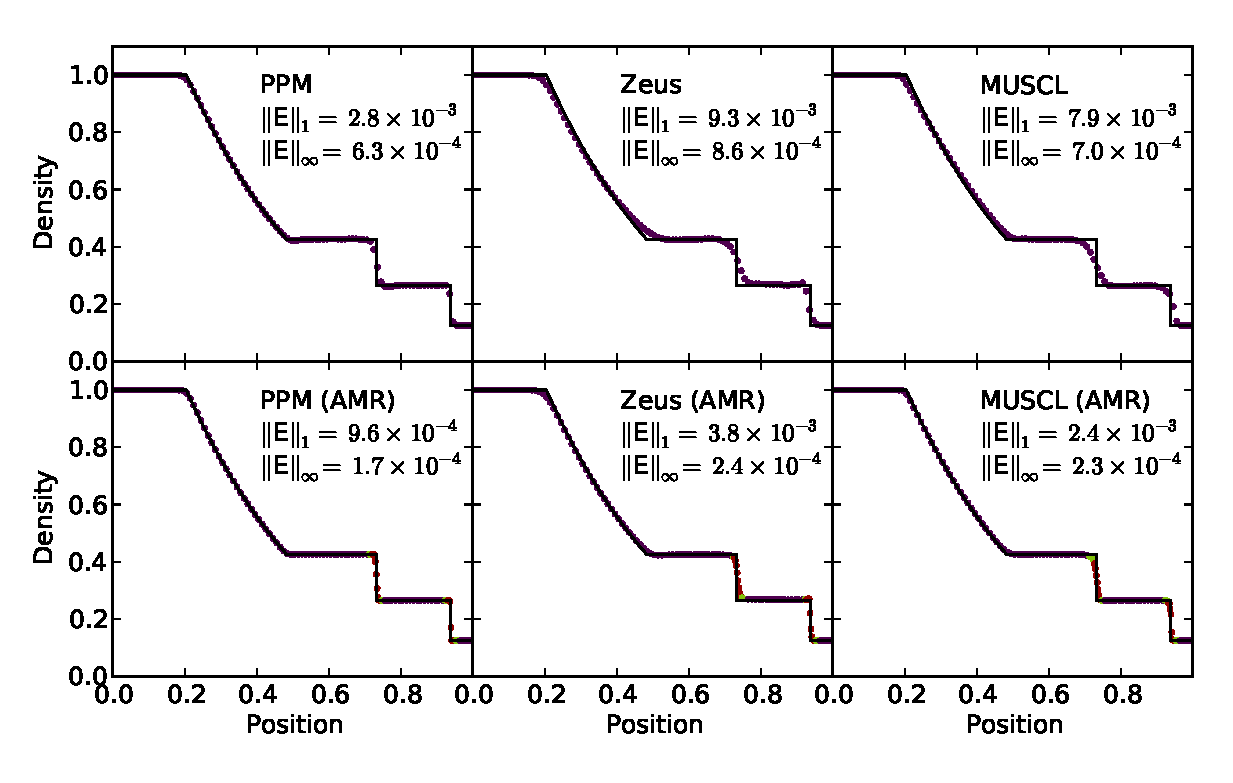
\includegraphics[width=\textwidth]{figures/SodShockTube.eps}
\caption{The density distribution of the classic Sod Shock Tube for three different solvers (from left to right) and with (bottom) and without (top) AMR.  In each case 100 zones are used on the root level and the results are shown at $t=0.25$.  All cells are plotted and color-coded by level (at the time shown, only small region surrounding the contact discontinuity and the shock are refined).  In each panel, we show the exact solution as a solid line and the $L_1$ and $L_\infty$ error norms in the upper right.}
\label{fig.sodshocktube}
\end{center}
\end{figure}


%%%%%%%%%%%%%%%%%%%%%%%%%%%%%%%%%%%%%%%
\subsubsection{Wave pool}
\label{sec.tests.wavepool}
\red{(Greg)}
Problem type 2, with AMR.  Tests reflections of waves at grid boundaries.

%%%%%%%%%%%%%%%%%%%%%%%%%%%%%%%%%%%%%%%
\subsubsection{Shock pool}
\label{sec.tests.shockpool}
\red{(Greg)}
Problem type 3, with AMR.  Tests passage of shock through a refinement boundary.

%%%%%%%%%%%%%%%%%%%%%%%%%%%%%%%%%%%%%%%
\subsubsection{Double mach reflection}
\label{sec.tests.doublemach}
\red{(Brian)}

The double mach reflection test is a classic two-dimensional test of
hydrodynamic algorithms, and was originally described in
\citet{1984JCoPh..54..115W} \citep[and more recently
in][]{2008ApJS..178..137S}.  In this problem (shown in
Figure~\ref{fig.doublemach}), a shock is injected at an angle to a
reflecting surface, and a jet appears along the reflecting surface.
The ideal solution is self-similar, and the appearance of this
solution is highly sensitive to numerical diffusion.  If numerical
noise is present, a Kelvin-Helmholz instability develops along this
jet and breaks the self-similarity.

In the test problem shown in Figure~\ref{fig.doublemach}, a 2D
simulation with $960 \times 240$ cells was formed with a domain of $x
= [0, 4]$ and $y = [0, 1]$.  We use an ideal gas equation of state of
$\gamma = 1.4$, a pre-shock density of 1.4, and a pre-shock specific
internal energy of $2.5/1.4$ (all in arbitrary units).  A Mach 10
shock is initialized with a shock normal that is 30$^\circ$ from the
x-axis and an initial position on the lower boundary of x$ = 1/6$.
The lower y boundary and right x boundary are reflecting; the left x
boundary is inflowing, and the upper y boundary has a time-dependent
boundary condition that allows the shock to propagate into the domain
as if it extends to infinity.  The simulation starts at t$ = 0$ and
runs until t$ = 0.205$ (arbitrary units), at which point the rightmost
extent of the shock should be at roughly x$ = 3$.  In this run, we use
the direct Eulerian implementation of the piecewise parabolic hydro
method, with diffusion, flattening, and shock steepening all turned
on.

It is instructive to compare Figure~\ref{fig.doublemach} to Figure 9
in~\citet{1984JCoPh..54..115W}.  By the end of the simulation, a dense
jet is apparent at the leading edge of the shock, propagating along
the x-axis.  The shape of this jet is sensitive to numerical
diffusion, and our figure compares favorably to the higher-order
images from Woodward \& Colella.

\begin{figure}
\begin{center}
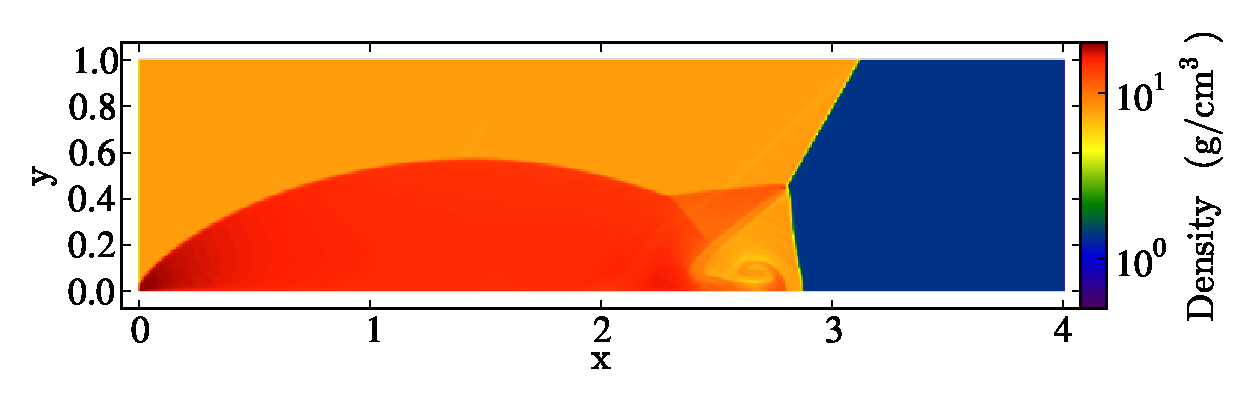
\includegraphics[width=0.8\textwidth]{figures/DoubleMachTest.eps}
\caption{Double mach test.}
\label{fig.doublemach}
\end{center}
\end{figure}

%%%%%%%%%%%%%%%%%%%%%%%%%%%%%%%%%%%%%%%
\subsubsection{Sedov Explosion}
\label{sec.tests.sedov}

\begin{figure}
\begin{center}
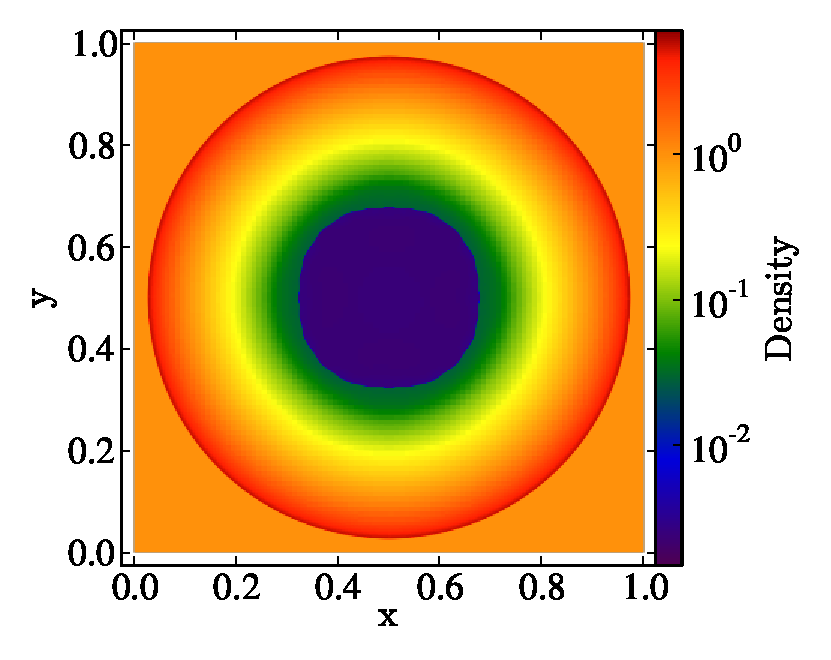
\includegraphics[width=0.4\textwidth]{figures/sedov-ppm-slice.eps}
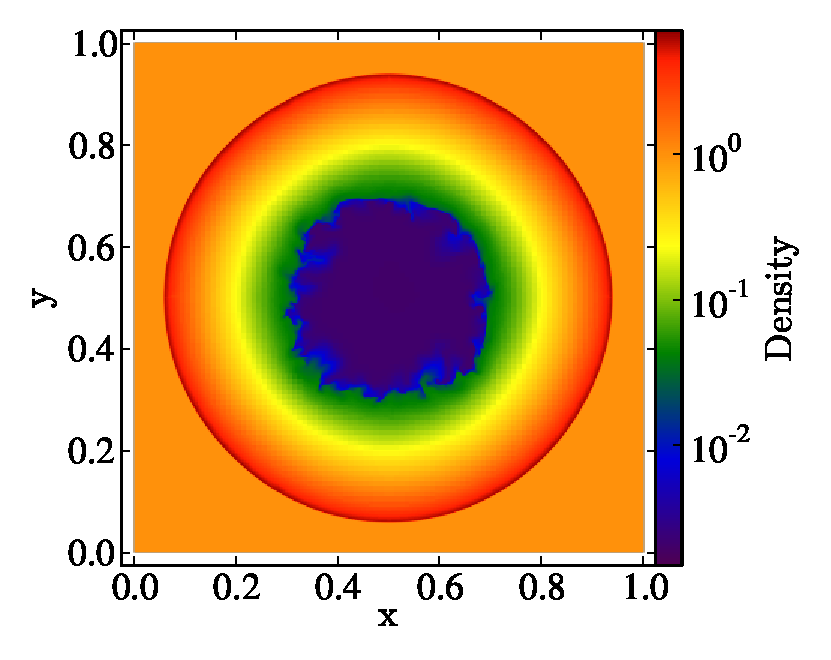
\includegraphics[width=0.4\textwidth]{figures/sedov-zeus-slice.eps}
\caption{Density slice from the Sedov Blast Test at $t =
0.07$. Left-hand image shows the results from PPM ({\tt HydroMethod =
0}), right-hand image shows the results from Zeus ({\tt Hydromethod =
2}). Notably, the Zeus shock front has progressed less far than forthe
PPM run. This is due to energy loss when conserving internal, not
total, energy.}
\label{fig.sedov1}
\end{center}
\end{figure}


\begin{figure}
\begin{center}
\includegraphics[width=\textwidth]{figures/sedov-profiles.eps}
\caption{Radially averaged profiles for the Sedov Blast Test at $t =
0.07$. Clockwise from top-left shows density, velocity, internal
energy and pressure.}
\label{fig.sedov2}
\end{center}
\end{figure}

The Sedov Blast Test \citep{Sedov1959} models an intense explosion,
initiated by depositing thermal energy into a homogenous distribution
of gas. The result is a strong spherical shock wave centered on the
point of energy injection.  This problem is a popular test of
astrophysical numerical codes for three reasons: Firstly, it is
particularly appropriate to astrophysics since it represents the
situation when a supernovae explosion occurs. Secondly, it has an
exact analytical solution whereby the shock front's radial position is
given by:

\begin{equation} r(t) =
\left(\frac{E_0}{\alpha\rho_0}\right)^{1/5}t^{2/5}
\end{equation}

\noindent where $E_0$ is the initial energy injection, $\rho_0$ is the
background density and $\alpha = 1.0$ for cylindrical symmetry and an
ideal gas with $\gamma = 1.4$. For the full derivation see
\citet{Sedov1959}. This solution makes it possible to assess how well
the code performs. Thirdly, the spherical shock is a challenging
problem for numerical codes (both grid and particle) since the shock
wave increases in size as the simulation progresses and its
symmetrical nature highlights any directional preferences that grid
codes can succumb to. The test presented here is the two-dimensional
version that is included in the Enzo distribution. The
three-dimensional results from this test, both for Enzo and three
other leading astrophysics codes, can be founds in \citet{Tasker2008}.

In the initial state, the box contains a homogenous distribution of
gas at a density of 1 (note that, in the absense of gravity, this
problem is scale-free and so without units). Thermal energy is
deposited into a single cell at the center of the box with $E_0 =
10.0$. The problem is completed in two dimensions with reflecting
boundary conditions (the default for Enzo) and uses a boxsize of side
$1$. For this problem, we selected a top grid of $100 \times 100$ and
four levels of refinement, placed based on shock location and the
slope in density and total energy (this corresponds to cell flagging
methods 1 and 3 in the Enzo parameter file). The exception to this
scheme is in the initial conditions where grids are placed directly
around the injection point. The results were assessed at $t = 0.07$,
which corresponding to a time just before the shock reaches the box
edge (see Figure~\ref{fig.sedov1}).

Figure~\ref{fig.sedov2} shows the radial profiles for the simulation
run with the PPM hydro-solver (blue dashed line) and the Zeus
hydro-solver (red dash-dot-dot line) together with the analytical
solution (black solid line). Clockwise from the top-left are density,
velocity, internal energy and pressure. PPM matches the analytical
solution extremely well for all quantities. However, Zeus' shock front
lags behind the analytical position. This can also be seen in the
slices shown in Figure~\ref{fig.sedov1}. The cause of this discrepancy
is that Zeus shows a substantial energy lost during the first few
timesteps and produces a diamond-shaped, rather than spherical,
shockfront during this time. After this, the code correctly conserves
energy but this intial energy loss remains clearly visible in the
position of the shock at $t = 0.07$. This problem was addressed
directly by \citet{Clarke2010}, who attributed the source of the issue
to this version of Zeus solving the internal, rather than total,
energy equation. In situations with strong energy gradients, this
choice caused an energy loss and the artificial viscosity produces the
direction-dependent shockfront shape. In their paper,
\citet{Clarke2010} presents results from an alternative version of
Zeus that conserves total energy. This problem is less marked for
smaller energy gradients and it should be noted that Zeus' stability
and speed make it a highly competitive choice, despite the
disagreements in this test.


%%%%%%%%%%%%%%%%%%%%%%%%%%%%%%%%%%%%%%%
\subsubsection{Point source gravity test}
\label{sec.test.gravitypointsource}
\red{(Greg)}
This is the TestGravity (problem 23) test problem.  It tests gravity around a point source, using fixed AMR.

%%%%%%%%%%%%%%%%%%%%%%%%%%%%%%%%%%%%%%%
\subsubsection{Orbit Test}
\label{sec.test.testorbit}
\red{(Greg)}
This is the TestOrbit problem (problem 29 for GB).  This tests gravity and particle integration (no hydro).

%%%%%%%%%%%%%%%%%%%%%%%%%%%%%%%%%%%%%%%
\subsubsection{Self-Similar infall test}
\label{sec.tests.infall}
\red{(Greg)}
Problem type 24.  This is a test based on Bertschinger's 1985 3D self-similar infall
solution, and tests gravity + hydro.

%%%%%%%%%%%%%%%%%%%%%%%%%%%%%%%%%%%%%%%
\subsubsection{Zel`dovich Pancake}
\label{sec.tests.pancake}

The Zel`dovich pancake \citep{1970A&A.....5...84Z} is particularly
relevant to cosmological simulations, because it includes many
features that are critical to structure formation: hydrodynamics,
expansion, and self gravity.  This problem represents an ideal,
isolated caustic formation, and is thus a useful proxy for much more
complicated structures in full 3-dimensional cosmological simulations
(such as the collapse of gas onto a cosmological halo or filament).

The initial conditions are simple, and we follow the prescription of
\citet{Anninos94}.  Assuming a flat cosmology, the density
perturbation is given by

\begin{equation}
\rho(x_l) = \rho_0 \big[ 1 - \frac{1+z_c}{1+z} \cos(k x_l) \big]
\end{equation}

with the internal energy of the gas set so that the entropy of the gas
maintains a constant value throughout.  The velocity perturbation is given by

\begin{equation}
v(x_l) = -H_0 \frac{1 + z_c}{(1+z)^{1/2}} \frac{\sin(k x_l}{k}
\end{equation}

In the equations above, $\rho_0$ is the background density, z$_c$ is a
free parameter and is the redshift at which the sheet forms a caustic
(i.e., 'pancakes'), z is the redshift of initialization, x$_l$ is the
Lagrangian mass coordinate, $k = 2 \pi / \lambda$ (where $\lambda$ is
the perturbation wavelength), and H$_0$ is the $z = 0$ value of the
Hubble constant.  Note that this solution is expressed in terms of
Lagrangian positions, so one needs to convert this into the Eulerian
coordinates, x$_e$, that are more useful to \enzo:

\begin{equation}
x_e = x_l - \frac{1 + z_c}{1 + z} \frac{\sin(k x_l)}{k}
\end{equation}

We note that the solution described above is exact up to the point of
caustic formation.  In Figure~\ref{fig.pancake}, we show the results
of a test of the AMR version of \enzo's Zel'dovich Pancake test.  A
one-dimensional box of length $64$~Mpc/h is initialized at z$ = 20$ in
an $\Omega_M = 1$ universe with h$ = 0.5$ and a background temperature
of 100~K, $\rho_0 = \rho_c$.  The simulation is initialized with 64
grid cells, refining by factors of four using criteria based on cell
mass and the presence of shocks, for a maximum of 2 levels (i.e., an
equivalent maximum resolution of 1024 grid cells).  The simulation was
evolved to z$ = 0$ using the PPM hydro method, with the final output
of the calculation being shown in Figure~\ref{fig.pancake}.

Figure~\ref{fig.pancake} shows the key features of this test problem.
The strong shocks and large density gradients are well-resolved, with
density and velocity jumps being well-delineated.  The key features of
this test problem can be resolved with far fewer cells -- simulations
including a mere 8 cells resolve the key features, as shown in
sections 3.3.4-3.3.5 of~\citet{1996PhDT........80B} -- but we choose a
higher resolution here for illustrative purposes.

\begin{figure}
\begin{center}
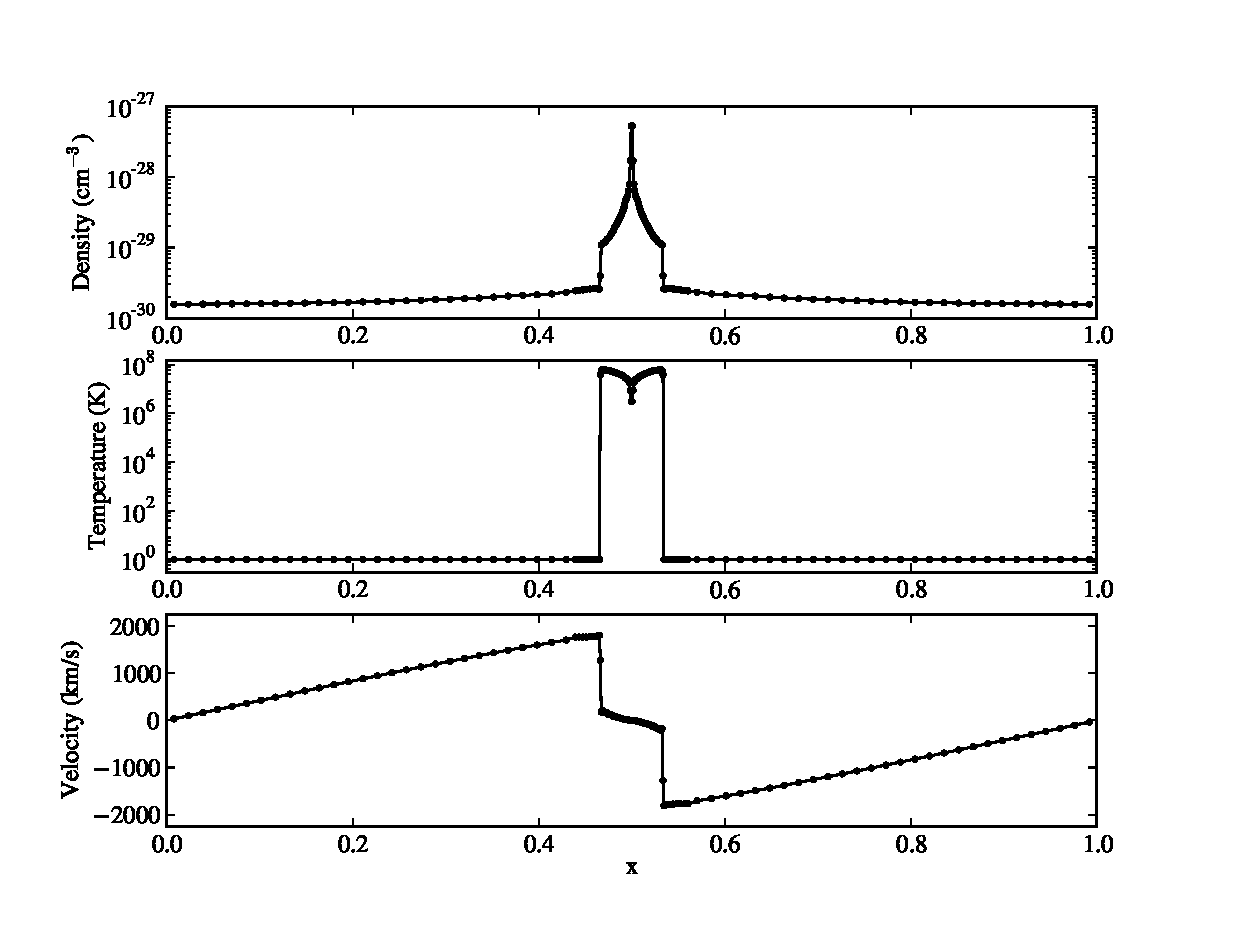
\includegraphics[width=0.8\textwidth]{figures/AMRZeldovichPancake.eps}
\caption{Zel`Dovich Pancake test shown at z$ = 0$, initialized in a
$\Omega_m = 1$ universe at z$ = 20$ on a one-dimensional grid having
64 cells, and further refined by factors of four based on cell mass
and the presence of shocks for up to two additional levels of mesh,
having a maximum effective resolution of 1024 grid cells.}
\label{fig.pancake}
\end{center}
\end{figure}


%%%%%%%%%%%%%%%%%%%%%%%%%%%%%%%%%%%%%%%
\subsubsection{MHD: Orszag-Tang Vortex}
\label{sec.tests.mhd}
Figure \ref{fig.orszag} shows the Orszag-Tang vortex problem, a
typical test problem for MHD \citep{Orszag79}.  The left panel shows
the MHD-CT result, while the right panel shows the Dedner result.
This test shows that small scale structure can be generated in MHD
from large scale initial perturbations.  The test begins with uniform
density, $\rho_0=25/36 \pi$ and pressure, $P_0=5/12 \pi$.  There is a
single rotational mode in the velocity, and two in the magnetic field:
${\bf v}_0 $ = (-sin(2$\pi$ y) $ \hat{x}$ , sin(2$\pi$ x) $\hat{y}$),
${\bf B}_0$ = (-sin(2 $\pi$ y) $ \hat{x},$ sin( 4 $\pi$ x )$\hat{y}$).
The simulation is evolved to t=0.48.  One can see that the structures
are accurately represented as compared to, for instance,
\citet{Toth00}, and that the resolution of shocks is comparable in
both methods.

{\emph Dave's note: I'll probably play around with these results in
future versions.}

\begin{figure}
\begin{center}
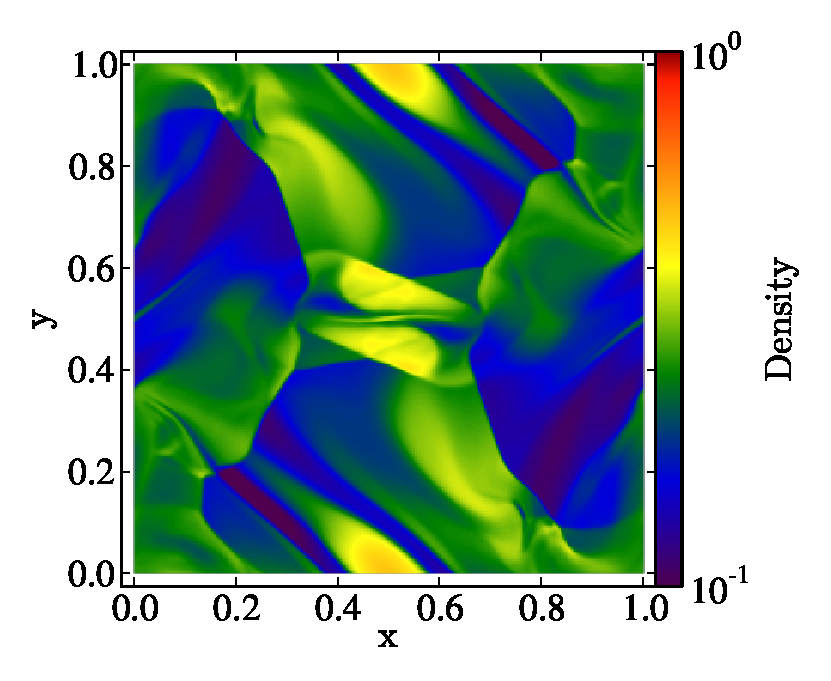
\includegraphics[width=0.4\textwidth]{figures/MHDCT_OrszagTang_Density.eps}
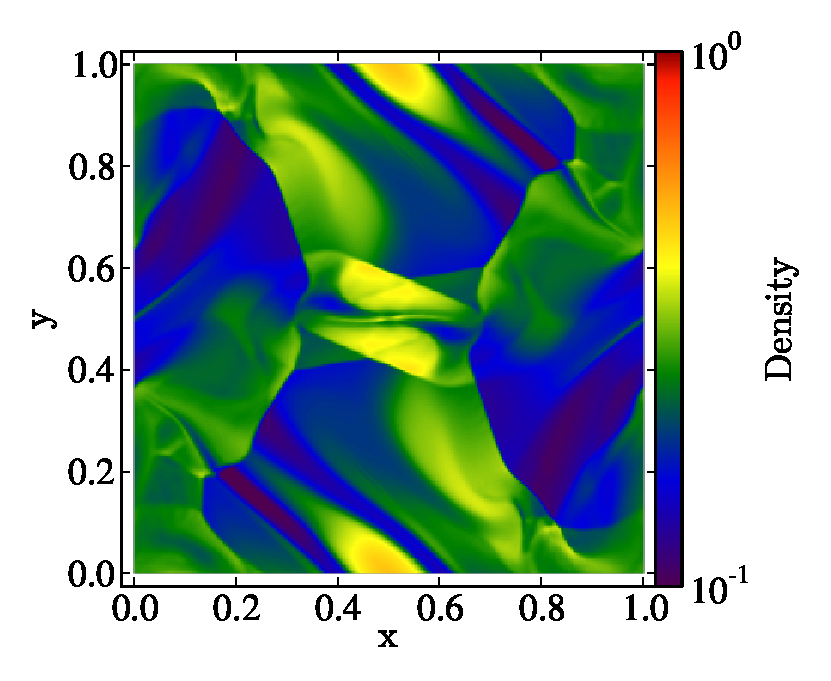
\includegraphics[width=0.4\textwidth]{figures/MHDDedner_OrszagTang_Density.eps}
\caption{TANG}
\label{fig.orszag}
\end{center}
\end{figure}


%%%%%%%%%%%%%%%%%%%%%%%%%%%%%%%%%%%%%%%
\subsubsection{One-zone collapse test}
\label{sec.tests.1-zone}
The one-zone collapse test simulates the collapse of a
self-gravitating gas cloud using a semi-analytic model for the
evolution of gas density and adiabatic heat input as a function of
time.  It is designed to test the chemistry and cooling modules over a
wide range in densities and over physically motivated timescales.
Because this test disables the hydrodynamic and gravity solvers and
uses a simple model for the density evolution, it is far faster than
running a true collapse simulation.  The density evolution is based on
the self-similar Larson-Penston \citep{1969MNRAS.145..271L,
  1969MNRAS.144..425P} solution for isothermal collapse with a
modification to account for the efficiency with which the heat
introduced by compression can be radiated away
\citep{1983ApJ...265.1047Y}.  Our implementation, described briefly
here, follows the work of \citet{2005ApJ...626..627O}, which one
should consult for further details.  The density evolution is given by 
\begin{equation}
\frac{d\rho}{dt} = \frac{\rho}{t_{col}},
\end{equation}
where the collapse timescale, $t_{col}$, is
\begin{equation} \label{eqn.tcol}
t_{col} = \frac{t_{dyn}}{\sqrt{1 - f}},
\end{equation}
and $t_{dyn}$ is the dynamical time, expressed as
\begin{equation}
t_{dyn} = \sqrt{\frac{3 \pi}{32 G \rho}}.
\end{equation}
The collapse timescale is altered from the dynamical time by the
factor, $f$ in Equation \ref{eqn.tcol}, which an approximation of the
ratio of the pressure to the force of gravity.  The value of $f$
depends on the effective adiabatic index, $\gamma_{ef} \equiv (\partial
ln\ p / \partial ln\ \rho)$, which we calculate by linearly extrapolating
from derivative values for the two previous timesteps.  For the value
of $f$, we use the piecewise function of \citet{2005ApJ...626..627O},
given by
\begin{equation}
f = \left\{
  \begin{array}{ll}
  0, & \gamma_{ef} < 0.83,\\
  0.6 + 2.5 (\gamma_{ef} - 1) - 6.0 (\gamma_{ef} - 1)^{2}, & 0.83 <
  \gamma_{ef} < 1,\\
  1.0 + 0.2 (\gamma_{ef} - 4/3) - 2.9 (\gamma_{ef} - 4/3)^{2}, & \gamma_{ef} > 1.
\end{array} \right.
\end{equation}
The specific energy evolves as
\begin{equation}
\frac{de}{dt} = -p \frac{d}{dt} \frac{1}{\rho} - \Lambda,
\end{equation}
where $\Lambda$ is the cooling rate in units of erg s$^{-1}$ g$^{-1}$
and energy, temperature, density, and pressure are related by the
ideal gas law.  Figure \ref{fig.onezone} shows an example of the
one-zone collapse test performed with an initial number density of 1
cm$^{-3}$ and temperature of 100 K using the 12 species chemistry
network with H, D, and He species and metal cooling rates calculated
with Cloudy.

\begin{figure}
  \begin{center}
    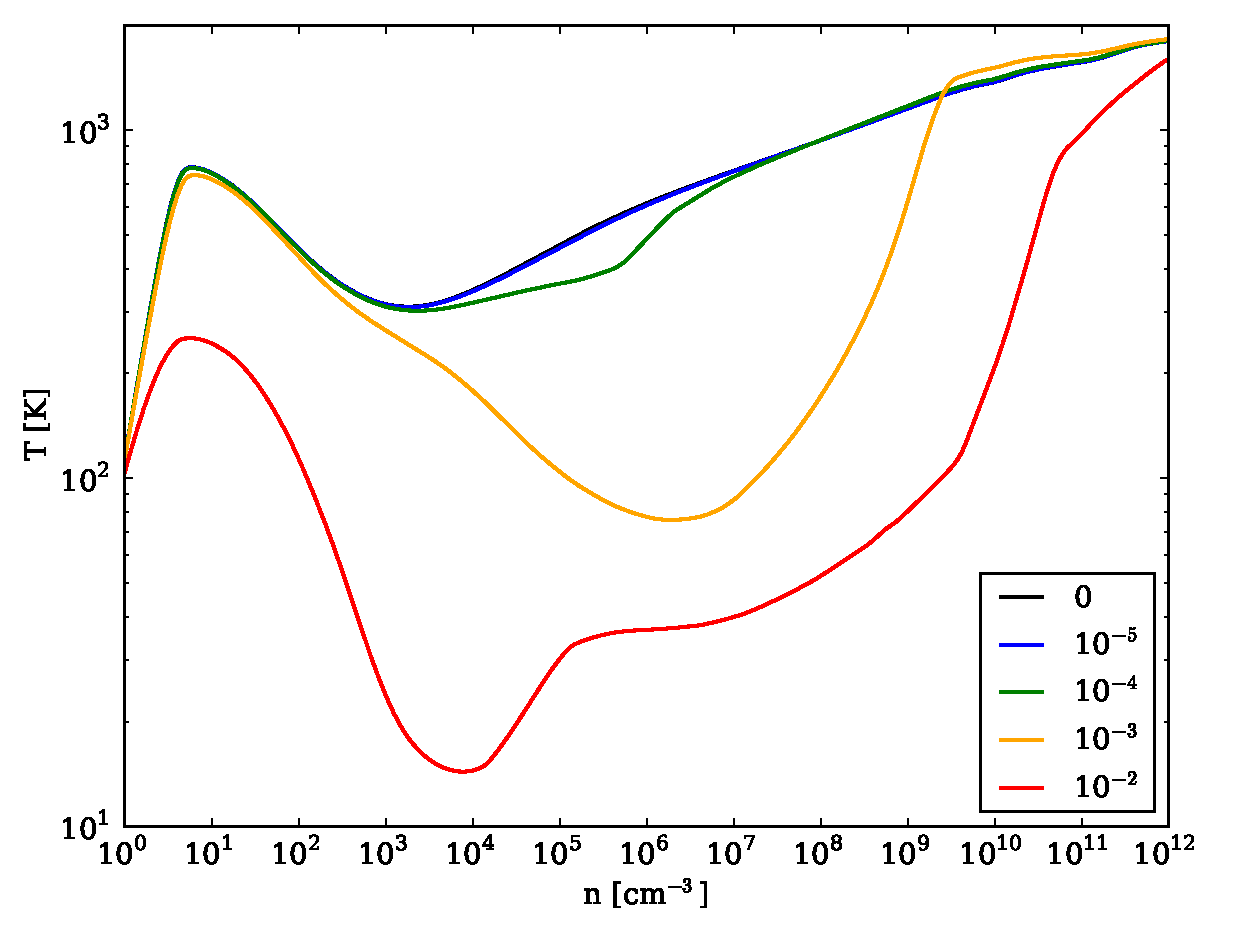
\includegraphics[width=1.0\textwidth]{figures/OneZoneCollapseTest.eps}
  \end{center}
  \caption{Evolution of temperature versus number density for a one-zone
    collapse test for gas at metallicities from 0 to 10$^{-2} Z_{\odot}$
    using the primordial chemistry network with tabulated metal cooling
    rates calculated with Cloudy.}
  \label{fig.onezone}
\end{figure}


%%%%%%%%%%%%%%%%%%%%%%%%%%%%%%%%%%%%%%%
\subsubsection{Photo-evaporation of a dense clump}
\label{sec.tests.raytracing}

The photo-evaporation of dense clumps is prevalent in radiation
hydrodynamics simulations, and this test problem examines the
ionization front propagation into the dense clump, shadowing effects
behind the clump, and the hydrodynamic response on the clump from
photo-heating.  The problem setup is the same as Test 7 in the
Cosmological Radiative Transfer Comparison Project
\citep{IlievEtAl2009} and \citet{Wise11_Moray}.  The simulation domain
is 6.6~kpc on a side with an ambient medium of pure neutral hydrogen
$n_{\rm H} = 2 \times 10^{-4}\; \cubecm$ and $T = 8000 \unit{K}$.  We
place a spherical overdensity in hydrostatic equilibrium with the
ambient medium.  It has a radius $r = 0.8 \unit{kpc}$, hydrogen
density $n_{\rm H} = 0.04 \cubecm$, and temperature $T = 40$ K, and it
is centered at $(x,y,z) = (5, 3.3, 3.3) \unit{kpc}$.  In
\citet{IlievEtAl2009}, all of the codes used a fixed $128^3$ grid to
ease the comparison, but in this test to demonstrate a higher
resolution AMR solution, we employ a $128^3$ grid with two additional
levels of refinement with cells with a baryon mass (method 2 in
\S\ref{sec:refinement_criteria}) greater than 1.5 being flagged for
refinement.  This test is run for 15 Myr.

This cloud is subject to radiation from a point source at the center
of the $y=0$ boundary with an ionizing photon luminosity
$\dot{N}_\gamma = 3 \times 10^{51}$ photons s$^{-1}$, corresponding to
a flux $F_0 = 10^6 \unit{photons s}^{-1} \unit{cm}^{-2}$ at the clump
surface closest to the radiation source.  The radiation source has a
spectrum of a $T = 10^5 \unit{K}$ blackbody, and we use four energy
groups with the following mean energies and relative luminosities:
$E_i = (17.98, 31.15, 49.09, 76.98) \unit{eV}, L_i/L = (0.23, 0.36,
0.24, 0.06)$ that are optimized to reduce errors in the solutions with
a full spectrum and energy discretization \citep{Mirocha12}.  Note
that this choice of energy groups is different from
\citet{Wise11_Moray}.  We use a minimum angular resolution of 10 rays
per cell and a constant radiative transfer timestep of 25 kyr.  Figure
\ref{fig:shadowing} depicts the clump after at $t = 15$ Myr with the
outer layers expanding after being photo-heated.  It also shows the
sharp shadowing effects of the dense clump in the neutral fraction
plot that is representative of ray tracing techniques.

\begin{figure}
  \centering
  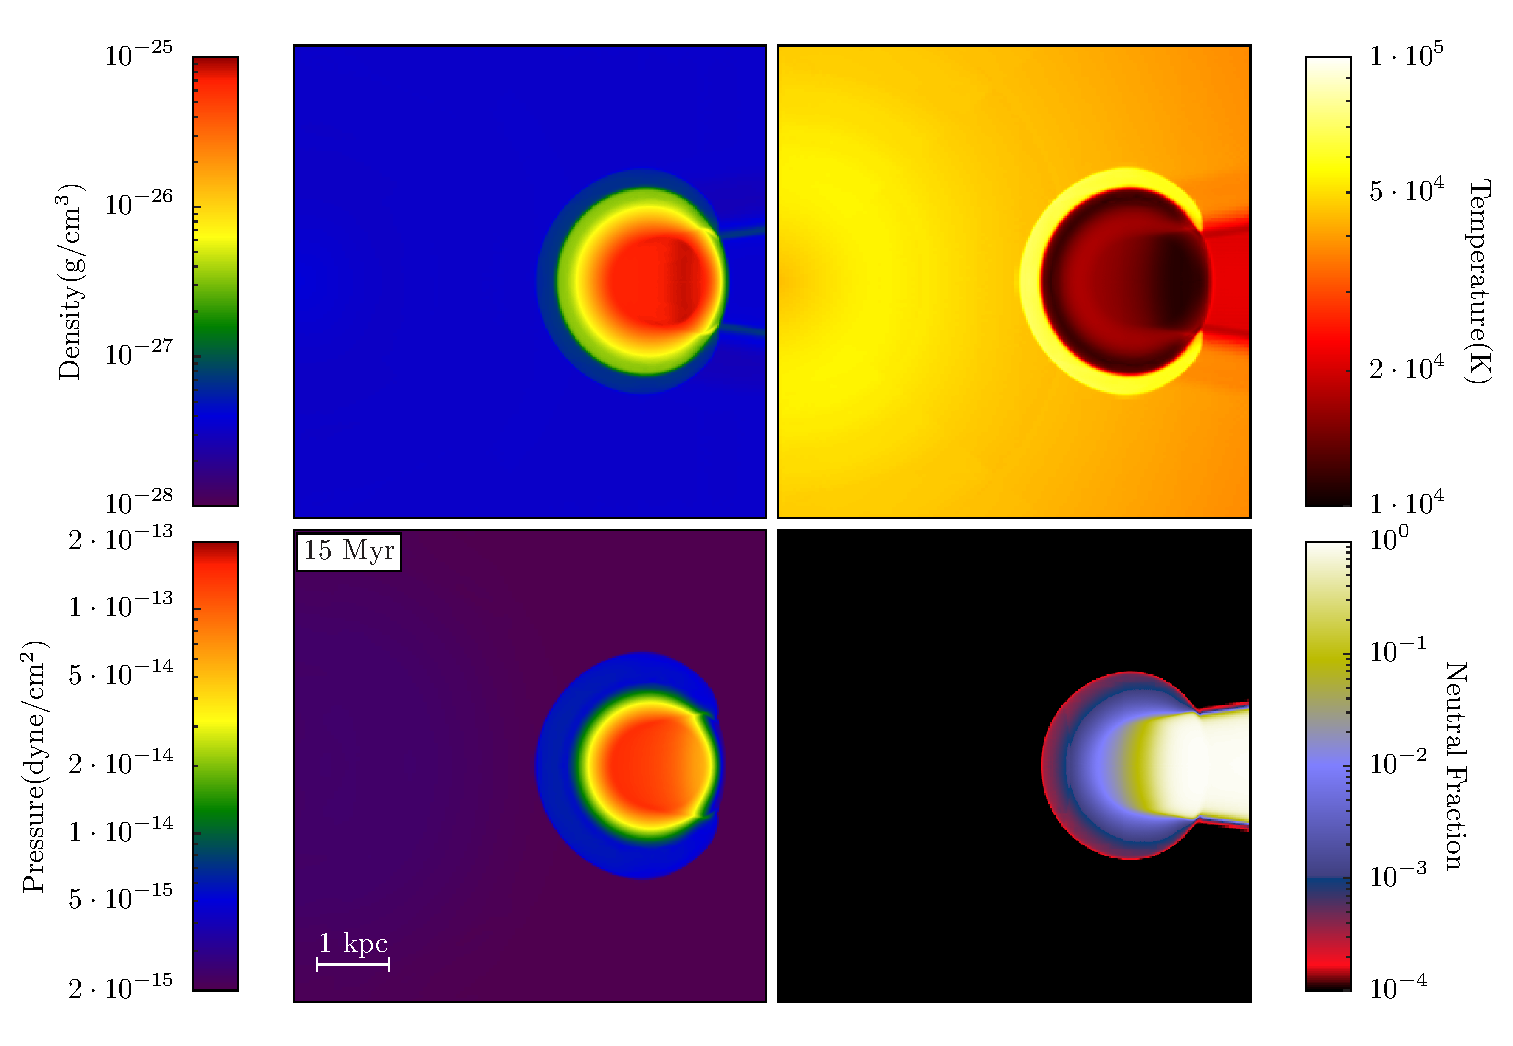
\includegraphics[width=1.0\textwidth]{figures/code-test-shadowing.eps}
  \caption{Photo-evaporation of a dense clump.  Clockwise from the
    upper left-hand side: slices through the clump center of the
    density, temperature, neutral fraction, and pressure.}
  \label{fig:shadowing}
\end{figure}

%%%%%%%%%%%%%%%%%%%%%%%%%%%%%%%%%%%%%%%
\subsubsection{Representative FLD test}
\label{sec.tests.fld}

\red{(Dan)}
One test for the implicit FLD: best/hardest one.



%%%%%%%%%%%%%%%%%%%%%%%%%%%%%%%%%%%%%%%

\subsubsection{Anisotropic Thermal conduction}
\label{sec.tests.conduct}

In a plasma, conduction takes place primarily due to electron motion.
In astrophysical environments such as the intergalactic and
intracluster media, with typical magnetic strengths of $\sim 1 \mu$G
and temperatures in the millions of Kelvin, the electron gyroradius is
very small compared to the scapes of interest in a cosmological
simulation.  As a result, electrons can only move \textit{along}
magnetic field lines, not perpendicular to them, which can result in
very interesting magnetohydrodynamical instabilities
\citep[e.g.,][]{2008ApJ...677L...9P,2008ApJ...688..905P}. 
 The correct modeling of this behavior can be quite challenging, and is described in 
Section~\ref{sec.num.conductions}.  Conduction in \enzo\ is calculated
in both an operator-split and directionally-split manner, and the
addition of heat transport solely along magnetic field lines requires
computation of cross-terms in the temperature derivative at cell
faces, which can add spurious oscillations in the temperature field in
regions where the temperature gradient is strong in more than one
spatial direction unless an appropriate flux-limiter \citep[such as that
of][]{1977JCoPh..23..263V} is chosen.

Figure~\ref{fig.conduct} shows a test that demonstrates the
correct behavior of anisotropic thermal conduction in \enzo.  We
initialize a two-dimensional, $256^2$ cell simulation having a physical
scale of 1 kpc on a side, a uniform density of 1 proton/cc, and a
background temperature of $10^6$ Kelvin.  Magnetic fields with a
strength of  B$_0 = 1 \mu$G are initialized such that the field lines form
circles around the center of the simulation volume, such that B$_x =
-B_0\sin(\theta)$ and B$_y = B_0\cos(\theta)$, where $\theta$ is the
angle measured from the $+x$ direction in a counterclockwise manner.
A Gaussian temperature pulse is injected at $(0.75, 0.5)$ (in units of the box
size), with a peak temperature of $10^8$ K and a FWHM of $0.015625$ of
the box size.  This initial setup is shown in the left panel of
Figure~\ref{fig.conduct}.  The simulation is then allowed to evolve
with \textit{only} anisotropic conduction turned on (e.g.,
no hydrodynamics or radiative cooling), and with a Spitzer fraction of
f$_{sp} = 1$.  

The right panel of Figure~\ref{fig.conduct} shows the state of the
simulation after 300 Myr.  Heat has clearly been transported only along
field lines -- there has been no diffusion perpendicular to the
magnetic field setup, which is critical for many studies involving
anisotropic thermal conduction.  No oscillations are seen in the
temperature field in regions where the fields are not aligned with the
grid, suggesting that the flux-limiter is operating as expected.

\begin{figure}
\begin{center}
\includegraphics[width=0.42\textwidth]{figures/aniso_conduction_initial_output.eps}
\includegraphics[width=0.4\textwidth]{figures/aniso_conduction_final_output.eps}
\caption{Two-dimensional anisotropic conduction test in a uniform,
constant temperature background with circular magnetic fields centered
on (0.5, 0.5).  The background medium has a density of 1 proton/cc and
a temperature of $10^6$~K.  At t$ = 0$ (left panel), a Gaussian heat
pulse is injected at (0.75, 0.5) with a FWHM of $0.015625$ (with all
numbers given in units of the box size) and a peak temperature of
$10^8$~K, and allowed to evolve without hydrodynamical motion (i.e.,
static gas) and no radiative cooling for 300 Myr.  At t$ = 300$~Myr
(right panel), heat has been transported along magnetic field lines
with no significant diffusion perpendicular to field
lines. Furthermore, there is no detectable oscillations in the
temperature in regions where the field is not parallel with the grids.}
\label{fig.conduct}
\end{center}
\end{figure}


%%% Local Variables: 
%%% mode: latex
%%% TeX-master: "ms"
%%% End: 


%% Section: parallelism and performance
\section{Parallel Strategy and Performance}
\label{sec.parallel}

\subsection{Parallel Strategy}

The current version of \enzo\ has been parallelized for distributed
memory platforms using the Message Passing Interface (MPI).  This is
done using a single grid object as the basic unit of parallelization.
Each grid object -- including all cell and grid data -- is fully
contained on a single processor\footnote{In this context, we use the
word {\it processor} to mean a basic distribution unit; this could be
either a core or a node, depending on details of the system.  Note
that the current version of Enzo is not threaded, although a hybrid
MPI + OpenMP version is currently under development.}.  
Parallelization is
accomplished by distributing grids amongst processors.  This is done
on the root grid using a simple tiling system, where the root grid is
split up into $N_{\rm root}$ tiles, with $N_{\rm root}$ typically
equal to the number of processors, $N_p$.

Load balancing on levels other than the root level (i.e., grids for
which the level $l > 0$) is different, as the refined patches are not
generally uniformly distributed.  Grids on refined levels are first
placed on the same processor as their parent to minimize
communication; however, this generally does not result in a
well-balanced computational load.  Therefore, the code has a number of options for
load balancing the grids on a given level. Each grid is assigned an
estimated computational load, generally equal to the number of cells in the grid (which,
empirically, is a good estimate of computational cost).  The first
load-balancing option is to move a grid from the processor with the
highest computational load to the processor with the lowest load, with the proviso
that only grids with load factors less than half the difference
between the highest and lowest loaded processors will be moved.  This
continues until the load ratio between the most-to-least loaded
processor is below 1.05 or until no suitable grid can be found to
transfer.  A second load balancing option uses a space-filling Hilbert
curve to order the grids by their approximate spatial position.  Then,
once the grids have a specific one-dimensional ordering, we can divide
up the grids into $N_p$ groups (with the division taking place as
equally as possible).  Load balancing is done separately for each
level.  Clearly load balancing is most successful if there are
significantly more grids than processors; however, small grids are
less efficient (because of their ghost zones), and so the code uses a
simple heuristic in order to split up grids until there are of order
10 grids per processor.  This generally results in good load-balancing
while not producing grids that are wastefully small.

Communication between processors is done using a non-blocking
communication strategy that allows overlap of communication and
computation.  This can be done efficiently because each processor
retains a copy of the entire hierarchy of grids, except that grids
that do not `live' on a given processor only contain meta data
(essentially location and size of the grid; such grids are denoted as
`ghost' grids).  Replicating the hierarchy means that all
communication of data from one grid to another can be identified by
each processor independently.  The metadata for `ghost' grids are
quite small and so the extra memory required is generally not onerous
unless very large numbers of grids are used (more than a few hundred
thousand grids).  A schematic of this distribution is shown in
Figure~\ref{fig.amr_hierarchy}.

Data is transferred through a three-step procedure that takes
advantage of the capabilities of the MPI library: (i) as the code
progresses, and data is needed from another grid on another processor,
the receiving processor posts an MPI non-blocking receive indicating
that it is expecting data; this outstanding receive is recorded in a
table, (ii) the sending processor calls the MPI non-blocking send
function, and then finally (iii) the receiving processor, after it has
carried out all the computation it can, waits for any MPI message to
arrive.  Each message is coded so that it can be matched with the
appropriate receive posted in the first step, and based on that, the
appropriate routine is called to processes the data.  Step (iii) is
repeated until there are no outstanding receives.

 

\begin{figure}
\begin{center}
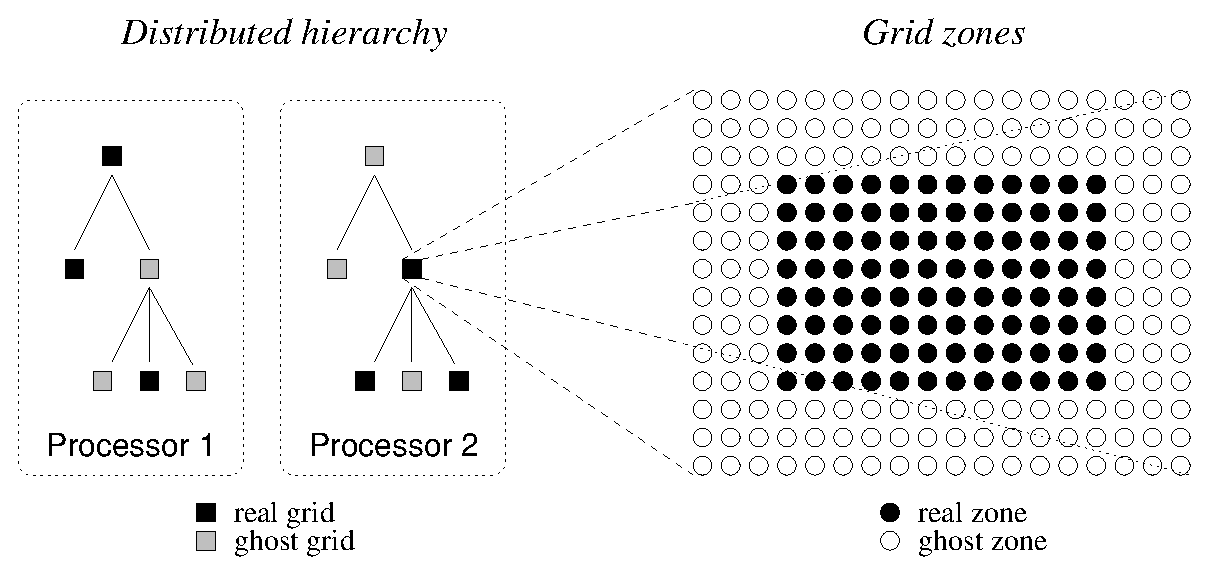
\includegraphics[width=0.5\textwidth]{figures/amr_hierarchy.eps}
\end{center}
\caption{\emph{Left:} Example of a simple, distributed AMR hierarchy
showing real and ghost grids.  \emph{Right:} Example 2D \enzo\ grid
showing real and ghost zones, as needed for the PPM hydro stencil. }
\label{fig.amr_hierarchy}
\end{figure}



% ----------------------------------

\subsection{Performance}
\label{sec.performance}

\subsubsection{Performance Measurement \& Instrumentation}

Because of the wide variety of simulations, methods, and uses of Enzo,
it is difficult to state in general terms which routines within the
code will be most costly during a given simulation.  As such, we have
designed a lightweight registering system that has been implemented
for the most commonly used routines (such as the hydrodynamic and
gravity solvers) as well as refinement level timers that measure the
time spent on each level.  Beyond this minimal set of routines, we
have designed a simple way for the user to modify the source by adding
\texttt{TIMER\_START("Your\_Routine\_Name")} and
\texttt{TIMER\_END("Your\_Routine\_Name")}.  These timers are created
and managed individually on each processor in an asynchronous fashion,
and contribute minimal computational, memory, and IO overhead.

At each complete root grid time step (or less often if specified),
each timer is then communicated to the root processor where it
calculates the mean, standard deviation, minimum, and maximum for each
of the timers across all processors.  For level timers, there are additional
attributes such as the number of cell updates, the current number of
grids, and the average cells updates per second per MPI process.  This
information is then 
output to a logfile.  This provides a simplified interface to the user
that can be used to diagnose performance issues as well as estimate a
given problem type's scalability.  In addition to the logfile, we have
developed a plotting interface for quickly producing figures that
process the data from the logfile.  These capabilities are described
in the online documentation, along with further discussion of the
performance measurement implementation.

\subsubsection{Unigrid scaling}
\label{sec:weak_scaling}

\begin{figure}
\begin{center}
\includegraphics[width=0.6\textwidth]{figures/enzo_unigrid_weak_scaling.eps}
\caption{\enzo\ weak scaling performance for a set of Lyman-$\alpha$
forest cosmology simulations with constant comoving spatial resolution
per grid cell, showing cell updates per second per processor 
plotted as a function of the number of root grid tiles of dimension
$128^3$ (R) in each dimension.  The number of MPI tasks is N$ = R^3$,
so R$ = 16$ on this plot corresponds to a $2048^3$ computational mesh
running on 4,096 MPI tasks.  This plot goes from R$ = 2$ (8 MPI tasks)
to R$ = 24$ (13,824 MPI tasks) on two supercomputers -- NICS Kraken
and ORNL Jaguar when they were Cray XT4 systems -- and using 1, 2 or 4
MPI processes per node, where each compute node contained a single
quad-core AMD Opteron CPU with a speed of 2.1 GHz on Jaguar and 2.3
GHz on Kraken.}
\label{fig.uniscale}
\end{center}
\end{figure}

It is advantageous to use \enzo\ in its ``unigrid'' (i.e.,
non-adaptive mesh) mode for a variety of problems, including
non-gravitating turbulence
\citep[e.g.,][]{2002ApJ...569L.127K,Kritsuk04}, the Lyman-$\alpha$ forest
\citep{2005MNRAS.361...70J,2009MNRAS.399.1934P}, or feedback of
metal-enriched gas from galaxies into the intergalactic medium
\citep{2004ApJ...601L.115N,2011ApJ...731....6S}.  Achieving good
scaling of the code in unigrid mode is relatively straightforward --
upon initialization, unigrid simulations are decomposed such that each
MPI process has a roughly equal subvolume (and thus an equal number of grid
cells), meaning that work is evenly distributed.  Communication
patterns for both the gravity solve (which uses a fast Fourier
transform) and the fluid solves (which transfer boundary information
between subvolumes) are predictable and straightforward, and
rebuilding of the grid hierarchy does not take place, removing a
substantial global operation and a great deal of communication.

Figure~\ref{fig.uniscale} shows \enzo\ weak scaling results for a
sequence of scaled unigrid Lyman-$\alpha$ forest calculations. These
calculations include dark matter dynamics, hydrodynamics using the
PPM solver, six-species non-equilibrium chemistry and
radiative cooling, and a uniform metagalactic ultraviolet background.
In this sequence of test calculations, we perform a weak scaling test
on up to 13,824 MPI tasks on the NICS Kraken XT4 and ORNL Jaguar XT4
supercomputers\footnote{These simulations were performed prior to
conversion of both machines to the current-generation systems}.  In
this test, each MPI task was given a $128^3$ root grid tile (i.e.,
$128^3$ grid cells containing baryon quantities) and, initially,
approximately $128^3$ dark matter particles.  The number of grid cells
on each processor 
was constant throughout the calculation; the number of dark matter
particles on each processor varies as they are moved from subvolume to subvolume as
structure evolves.  The grid resolution was kept at a constant
comoving size of $\simeq 40$~kpc/h, and as the core count was
increased, so was the simulation volume.  On each machine, a compute
node contained a single AMD Opteron quad-core chip (2.1 Ghz on Jaguar;
2.3 Ghz on Kraken) with 2 GB/memory per core (8 GB/total per node).
Both machines used the SeaStar2 interconnect.  In the scaling study,
calculations were run with 1, 2, or 4 MPI tasks per node.  The figure
shows cell updates per second per MPI process; perfect scaling would
be a horizontal line.

As can be seen in Figure~\ref{fig.uniscale}, the unigrid weak scaling
performance of the code is extremely good for this problem, with only
a 20\% decrease in cell updates per second per MPI task as the code is scaled from
8 to 4,096 MPI tasks, and a 40\% decrease in performance overall going
from 8 to 13,824 (or $24^3$) MPI tasks.  We speculate that this
decrease is likely to be partially due to global MPI communications
used to, e.g., calculate the overall timestep of the simulation, and
also likely due to load imbalances due to increasing cosmological
power (and thus an increasingly uneven distribution of dark matter
particles between MPI tasks at late times) as the simulation volume
grows.  We also observe that a systematic difference in speed can be
seen between the two machines, which can be attributed primarily to
the slightly faster CPUs on Kraken at th etime (2.3 Ghz, vs. 2.1 Ghz
on Jaguar).  The difference in speed when using different numbers of
MPI tasks per node can be attributed primarily due to differences in
competing usage of shared cache on the quad-core chips used on this
machine.

Broadly, excellent scaling in \enzo's unigrid mode is seen for a
variety of problems as long as each compute core is given an adequate
amount of work to do.  For cosmological simulations, this value has
been empirically determined to be roughly $128^3$ cells per core.  If
fewer cells per core are used, the CPU is essentially data-starved,
and poor scaling is observed due to computing units being idle while
waiting for information to be communicated from other processes (for,
e.g., boundary information or gravity solves).  Substantially larger
cell counts per core would in principle help scaling by reducing the
amount of inter-process communication needed, but larger cell counts
are typically impractical on most machines due to memory limits.

As a final point, we observe that scaling at larger core counts has
been measured, but only with an experimental hybrid-parallel (MPI +
OpenMP) version of \enzo.  Using this version, scaling comparable to
that shown in Figure~\ref{fig.uniscale} was seen on up to 98,304 cores
on the NICS Kraken XT5 (an upgraded version of the XT4 machine used
for the scaling study shown in the figure), using 2-8 OpenMP threads
per MPI process.  Hybrid parallelism has the potential to
substantially improve scaling by reducing the amount of communication
per grid tile (as described in the previous paragraph); however, the
optimal ratio of OpenMP threads per MPI task seems to vary
substantially between computational platforms and astrophysical
problems/required \enzo\ physics modules, and thus we hesitate to
provide strict guidelines here.

\subsubsection{AMR scaling}

\begin{figure}
\begin{center}
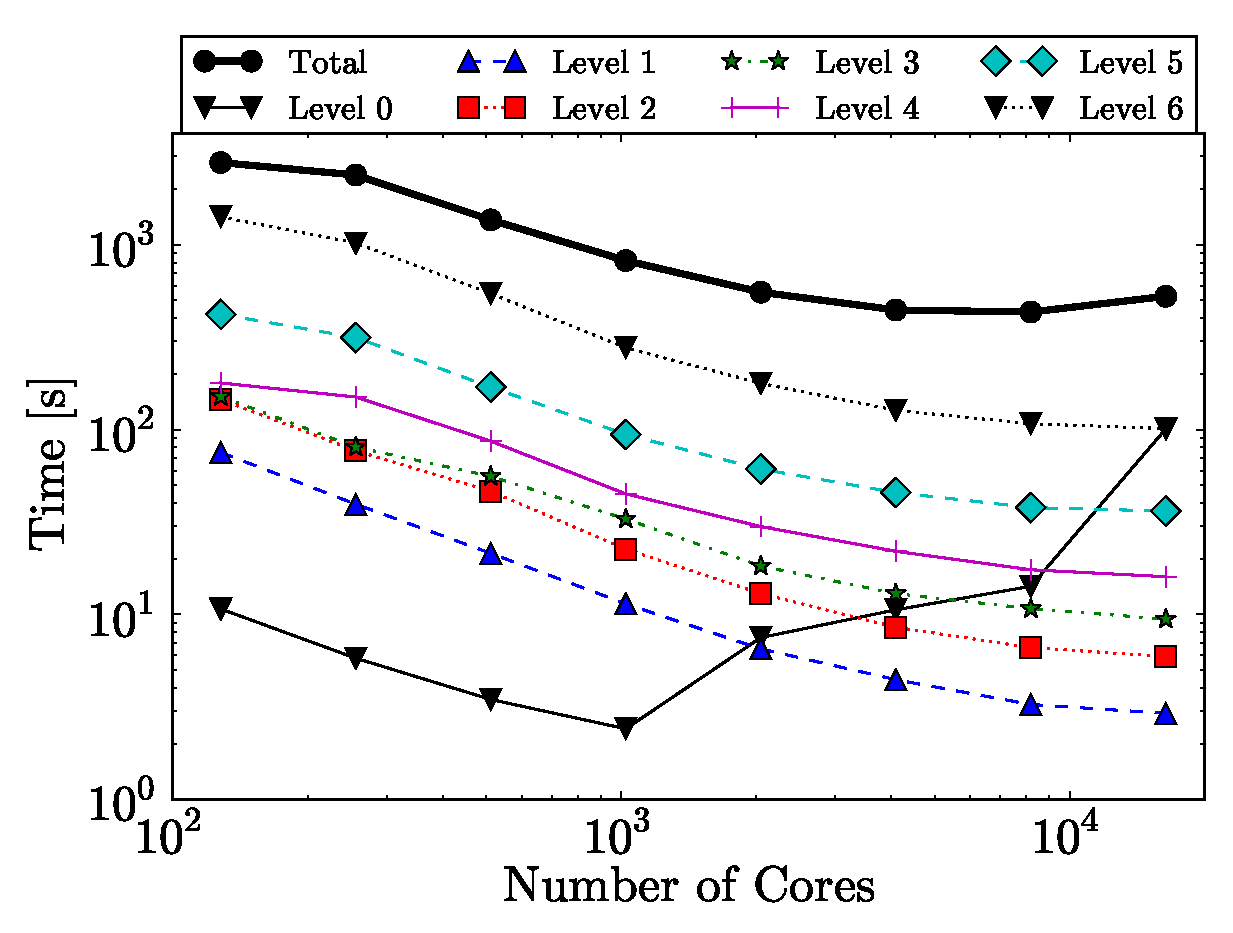
\includegraphics[width=0.48\textwidth]{figures/strong_scaling_levels.eps}
\hfill
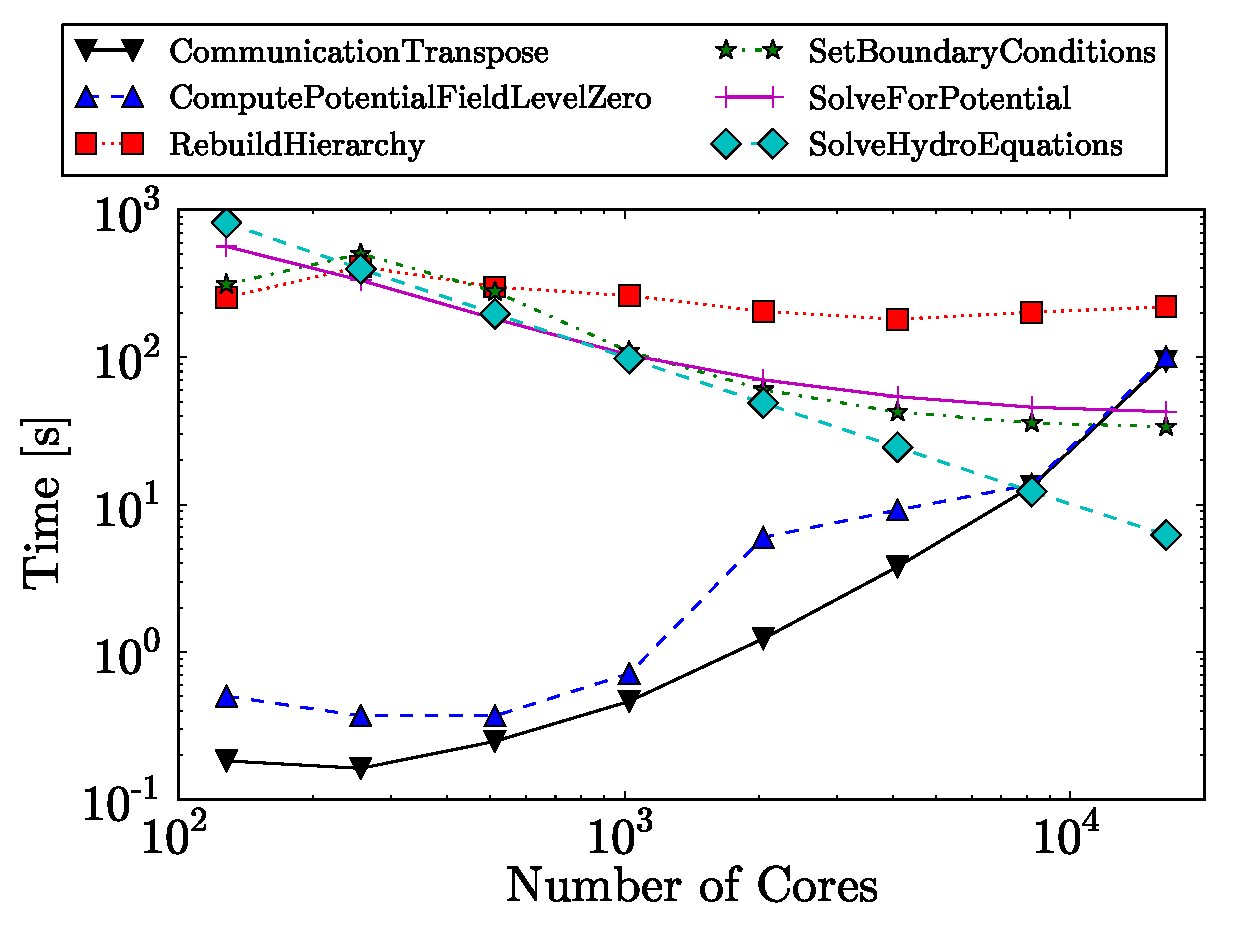
\includegraphics[width=0.48\textwidth]{figures/strong_scaling_routines.eps}
\end{center}
\caption{\emph{Left:} Strong scaling test of a 512$^3$ AMR
cosmological calculation.  The root grid scaling is not representative
of the true strong scaling of Enzo because the root grid tiles are not
repartitioned when a simulation is restarted with additional cores.
The weak scaling test in Figure \ref{fig.uniscale} is more
representative of the scaling on the root level.  The performance in
the refined levels show good strong scaling up to 2,048 cores.
\emph{Right:} Time spent in representative major routines in the same
AMR calculation.}
\label{fig:strong_scaling}
\end{figure}

Many astrophysical problems, such as cosmological galaxy formation
\citep{2012ApJ...749..140H}, high-resolution disk galaxy simulations
\citep{2011ApJ...738...54K}, high-redshift \citep{2009Sci...325..601T}, and present-day
star formation \citep{Collins12a}, involve multi-scale physics that
span several orders of magnitude in both space and time.  In these
situations, using Enzo in its adaptive mesh refinement mode is
beneficial.  Because the adaptive grid hierarchy is dynamic, grid
boundaries and, thus, communication patterns can be unpredictable,
hindering strong scaling to high core counts.

Figure \ref{fig:strong_scaling} shows strong scaling results from a
single 50 Mpc/h cosmology simulation run on $N_{\rm core}$ compute
cores, ranging from 128 to 16,384 cores at power-of-two intervals.  It
was run on the NICS Kraken XT5 supercomputer, which has two AMD
Opteron hexa-core processors with 16 GB of memory per compute node.
The simulations that utilized 128, 256, and 512 cores were executed on
128 nodes because of the memory requirements.  The higher core count
simulations were run with 8 cores per node.  This simulation would not
run with 12 cores per node because of the memory overhead associated
with the grid hierarchy being duplicated on each MPI process.
However, this overhead is greatly diminished if a hybrid-parallel (MPI
+ OpenMP) approach is used.

This simulation includes dark matter dynamics, hydrodynamics using the
piecewise parabolic method, six-species non-equilibrium chemistry and
radiative cooling, and a uniform metagalactic ultraviolet background.
The simulation uses the space-filling curve method for load balancing
the AMR grids.  It has a $512^3$ root grid that is divided into 512
tiles, and 6 additional AMR levels are used.  We perform these scaling
tests when the simulation reaches $z=4$, where the AMR grid hierarchy
is well-developed and is thus a reasonable representation of AMR
simulation behavior in general.  The results shown in Figure
\ref{fig:strong_scaling} come from a single root-level timestep
of $\Delta t = 2.1\, \textrm{Myr}$.  At this time, there are $3.04 \times
10^5$ AMR grids, $9.03 \times 10^8$ ($\sim 967^3$) computational
cells, and $1.34 \times 10^8$ dark matter particles in total.  The
breakdown of the number of AMR grids, cells, timesteps, and number of
cell updates on each level is shown in Table \ref{tab:amr_scale}.

%%%%%%%%%%%%%%%%%%%%%%%%%%%%%%%%%%%%%%%%%%%%%%%%%%%%%%%%%%%%%%%%%%%%%%%%
\begin{table*}
  \begin{center}
  \caption{Strong scaling test computational details}
  \begin{tabular*}{0.9\textwidth}{@{\extracolsep{\fill}}c c c c c}
    \tableline\tableline
    {Level} & {$N_{\rm grid}$} & {$N_{\rm cells}$} & {$N_{\rm up}$} &
    {$N_{\rm timesteps}$}\\
    \tableline
    0 & 512 & $1.34 \times 10^8$ & $1.34 \times 10^8$ & 1\\
    1 & 61,868 & $4.01 \times 10^8$ & $4.01 \times 10^8$ & 1\\
    2 & 91,182 & $1.99 \times 10^8$ & $5.96 \times 10^8$ & 3\\
    3 & 59,932 & $7.62 \times 10^7$ & $5.34 \times 10^8$ & 7\\
    4 & 40,700 & $3.32 \times 10^7$ & $5.65 \times 10^8$ & 17\\
    5 & 28,346 & $2.76 \times 10^7$ & $1.36 \times 10^9$ & 49\\
    6 & 19,771 & $2.80 \times 10^7$ & $5.25 \times 10^9$ & 187\\
    \tableline
    Total & 302,311 & $9.03 \times 10^8$ & $8.83 \times 10^9$ & --\\
  \end{tabular*}
  \parbox[t]{0.9\textwidth}{\textbf{Note.} --- Data shown at $z=4$ for
    a root grid timestep of 2.1~Myr.  
    Col. (1): AMR Level. Col. (2):
    Number of grids. Col. (3): Number of computational
    cells. Col. (4): Number of cell updates. Col. (5): Number of
    timesteps.}
  \label{tab:amr_scale}
  \end{center}
\end{table*}

%%%%%%%%%%%%%%%%%%%%%%%%%%%%%%%%%%%%%%%%%%%%%%%%%%%%%%%%%%%%%%%%%%%%%%%%

The left panel in Figure \ref{fig:strong_scaling} shows the
computational and communication time spent on each level.  In the AMR
levels, there exists good strong scaling up to 2,048 cores, and
marginal speed-ups are found at 4,096 cores.  On the root-grid level,
there exists good scaling up to 1,024 cores, but the performance
dramatically decreases at higher core counts.  This occurs because the
root grid is not re-partitioned into $N_{\rm core}$ tiles when the
simulation is restarted with a different core count.  This feature can
be easily implemented and is planned in the next major release of
Enzo, where scaling results would be similar to the weak scaling shown
in \S\ref{sec:weak_scaling}.  The right panel in Figure
\ref{fig:strong_scaling} shows the time spent in some representative
major routines in Enzo.  The local physics routines, for example
\texttt{SolveHydroEquations}, exhibit perfect strong scaling because
they involve no communication.  By investigating the scaling behavior
in each routine, it is clear that the communication in the
\texttt{SetBoundaryConditions}, \texttt{SolveForPotential} (multi-grid
solver in AMR levels), and \texttt{RebuildHierarchy} are responsible
for the lack of strong scaling at $N_{\rm core} \ga$~4,096 in this
particular simulation.  The transpose of the root grid tiles are
responsible for the performance decrease because it is not optimized
for situations where the number of tiles is greater than the number of
MPI processes.  These results are directly applicable to simulations
with similar computational demands.  In simulations with fewer
computational cells, strong scaling will cease at a smaller core count
because the CPUs will become data-starved more quickly, and the
opposite occurs with larger simulations.


\subsubsection{An Approximate Time and Memory Scaling Model}

In this section, we develop a simple, approximate model to estimate
the computational time and memory required to complete a given
calculation.  Note that we are {\it not} trying to model parallel
performance (which was discussed in the previous section), but have an
even simpler goal: to determine how to scale computational time
estimates as we increase the simulation resolution.  This is a
straightforward thing to do in codes that use static grids, as the
computational effort per time step is constant.  However, for an AMR
calculation, the number of grids that will be generated during the run
is not known in advance, and so the CPU time per problem time can vary
drastically throughout the calculation.  For example, at the beginning
of the simulation when the densities are nearly uniform, only the
static grid is required and the calculation progresses rapidly.
However, as structure forms and dense clumps are generated, the number
of grid points swells by orders of magnitude (an increase of $10^3$ is
not uncommon) and most of the CPU time is consumed at late times.
Therefore, simply performing a few steps at the beginning of the
calculation does produce a good estimate of the required CPU time.

Nevertheless, we can try to determine how the compute time scales for
a given run as we increase the resolution.  First, we neglect
particles and concentrate on the time taken by the grids, which can be
justified both theoretically and empirically\footnote{Since the
potential is calculated on the grid, the only particle costs are:
depositing mass to the grid, interpolating accelerations, and updating
particle positions and velocities.  These are relatively
computationally inexpensive operations.}.  Second, we break the
problem down slightly, and examine the scaling over a short enough
period of time that the grid structure does not change significantly
(i.e. the number of grids at each level remains approximately
constant).  We then assume that the whole run scales in the same way,
or in other words, that changes in the resolution affect the
simulation in the same way at each time step.  This is usually a good
approximation, as the most costly parts of the calculation typically
don't change their characteristics substantially between timesteps.

To make progress, we assume that the computational cost to advance a
single cell by one timestep is a constant.  This can be incorrect if
the chemistry solver requires many iterations, but is usually fairly
accurate.  For a unigrid calculation, the time would by proportional
to $N_{\rm root}^4$ since the number of cells scales as $N_{\rm
root}^3$ and, assuming the Courant condition is the 
factor that controls the time step, the number of steps to advance the
calculation over a given time interval is
proportional to $N_{\rm root}.$ Therefore, to advance a hierarchy a
given time interval, we find, accounting for all levels and using a refinement
factor of 2,
\begin{equation} t_{\rm SU} = C_1 \sum_l f_l N_{\rm root}^4 2^{4l}
\end{equation} where $C_1$ is a constant, which can be thought of as
the time taken to advance a single cell.  The factor $f_l$ is the
fraction of the volume on a given level that is actually refined.  By
definition $f_0 = 1$, and $f_l \le 1$.  In writing down this equation,
we neglect a number of costs that are not directly proportional to
cell count, including communication between processors, the $\log{N}$
factor for the root grid FFT, cache misses, optimizations, and other
costs associated with processing the hierarchy.  The first item on
this list, in particular, is clearly important for large processor
counts; however, we neglect parallel considerations in this section.

Note that unless $f_l/f_{l+1} < 1/16$ (i.e. if less then about 6\% of
a given level is further refined), the cost per level will increase
with level.  A key question, therefore, is the value of $f_l$ for each
level.  Unfortunately, this depends strongly on the simulation being
run.  In Figure~\ref{fig:scaling}, we show the values of $f_l$ for
three simulations: two cosmological runs with varying box size, and a
third simulation focusing on a single disk galaxy.

\begin{figure}
\centerline{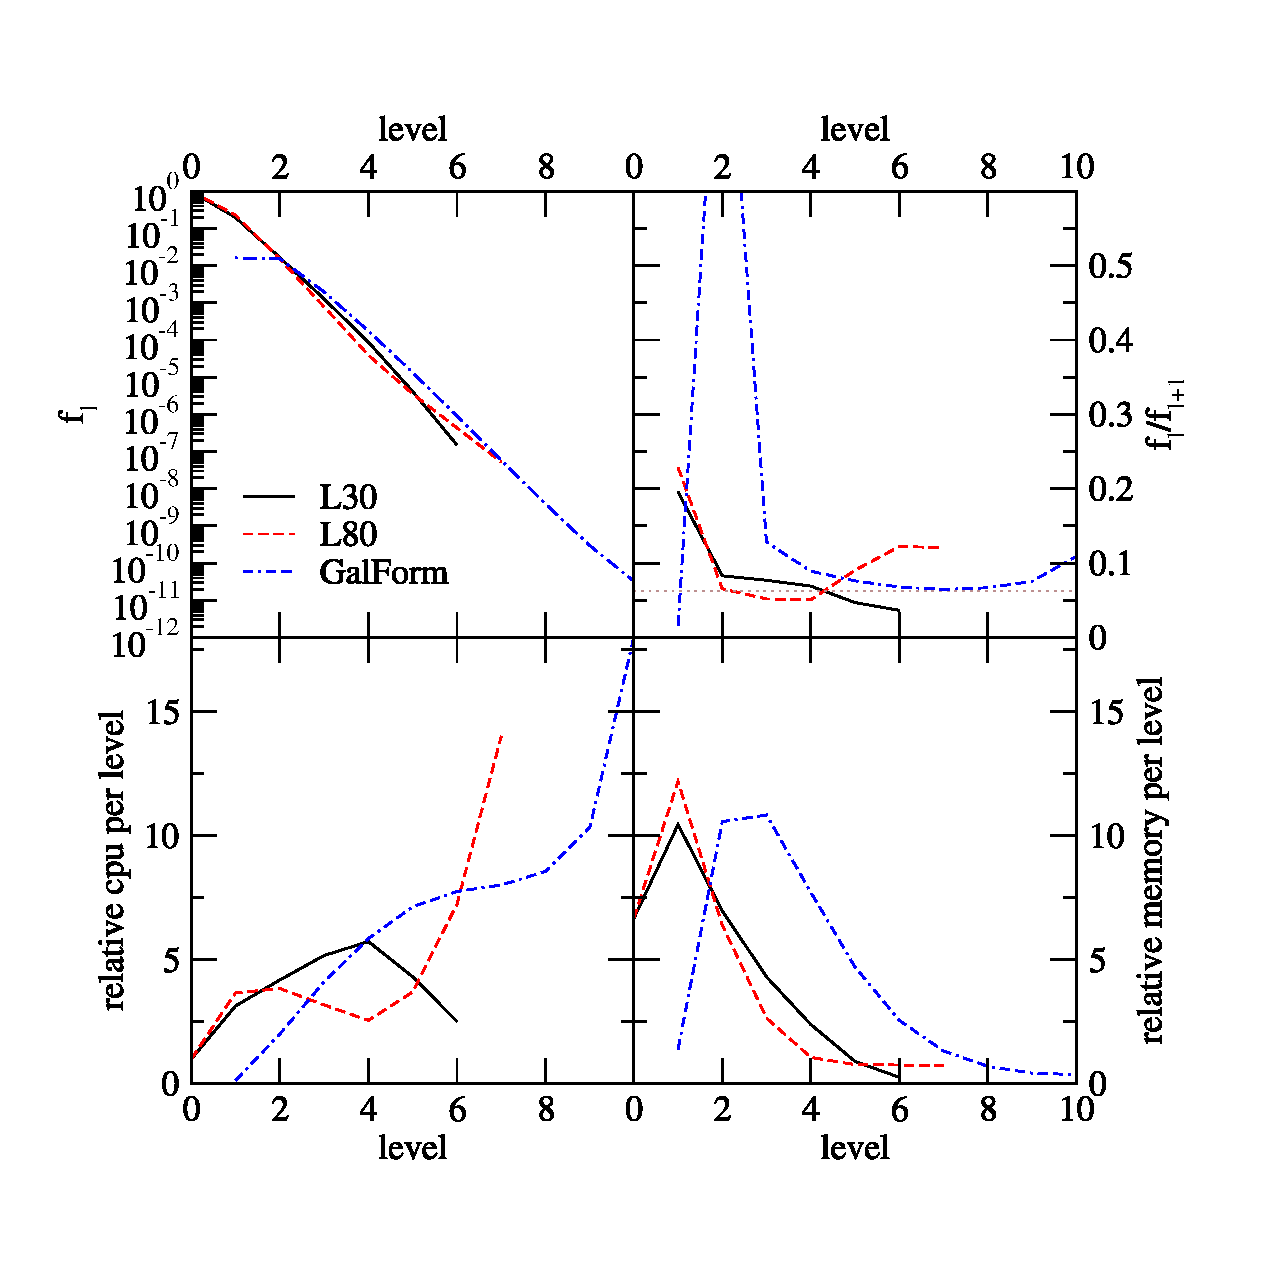
\includegraphics[width=0.7\textwidth]{figures/scaling_plot2}}
\caption{This figure shows (clockwise from upper left), the covering
fraction $f_l$ of the grids on a given level $l$, the ratio of
$f_{l}/f_{l+1}$, the relative memory usage of each level (normalized
by the memory usage of level 0), and, in the lower-left panel, the
relative CPU usage of each level, again normalized by $l=0$.  In each
panel, three curves are shown: the solid black and long dashed red are
two cosmological simulations with box sizes of 30 h$^{-1}$ Mpc and
80h$^{-1}$ Mpc respectively.  The dot-dashed blue line is for a
non-cosmological simulation of a ram-pressure stripped galaxy.  In the
top-right panel, there is a line at the critical ratio of 0.06, which
determines if the next finer level ($l+1)$ takes more (above) or less
(below) CPU time than level $l$.}
\label{fig:scaling}
\end{figure}

As, the figure demonstrates, the $f_l$ values all show a sharp decline
with level, dropping as power-laws with the level $l$.  Focusing first
on the ``refine-everywhere" cosmological runs, which both show similar
behavior despite the different box sizes and redshifts at which we
collect the data.  In fact, we find these results are very typical for
cosmological runs, with only slight variations depending on the exact
problem that is being simulated.  The top-left panel
shows the ratio of $f_{l}/f_{l+1}$ which, remarkably, hovers around
the critical value of 0.0625 determined earlier.  This implies that
the relative CPU usage of each level, shown in the lower-left panel,
is nearly flat, and that going to additional levels of refinement only
increases the amount of calculation by a factor of roughly $1/l_{\rm
max}$.  Even in the most extreme case, the L80 run, the last level
adds only 25\% to the computation time.

The memory used by each level, on the other hand, scales as
\begin{equation}
{\rm memory} = C_2 \sum_l f_l N_{\rm root}^3 2^{3l}
\end{equation}
and the terms in this sum are shown in the bottom-right panel of
Figure~\ref{fig:scaling}.  This demonstrates that the memory usage is
dominated by the top three levels, and adding additional levels 
adds minimally to the memory usage of the run.  We have empirically
tested this scaling for cosmological simulations and found it to be
reasonably accurate (although the increase is typically slightly
larger than found here, usually 30-50\%, probably because of
less-than-ideal parallel scaling).

The physical reason for the $f_{l+1}/f_l$ ratios found in the
cosmological simulations appears to be due to a combination of the
density structure of individual clouds, and the distribution of the
clouds themselves.  In particular, we note that for a $\rho \propto
r^{-2}$ density profile, the Lagrangian refinement criteria typically used in
such simulations produces an $f_{l+1}/f_l$ ratio of 1/8 for a single,
resolved cloud.  Of course, at some point we would resolve the flat
density of individual clouds and the ratio would climb, making further
refinement more costly; however, we are not yet in this regime in this
example.

These conclusions are, however, highly dependent on the type of run
being performed.  We contrast this cosmological case to the simulation
of a galaxy formation run, as shown by the dot-dashed curves in
Figure~\ref{fig:scaling}.  Note that grid levels 1 and 2 in this simulation are statically
refined to ensure that the Lagrangian volume of the galaxy halo is resolved
to at least level 2 at all times. More importantly, the
$f_{l+1}/f_{l}$ ratio of the highest levels are systematically
slightly larger than the critical 0.0625 value, indicating that the
CPU time is dominated by the most refined levels, as shown in the
bottom-left panel.  The memory usage is dominated by levels 2 and 3,
the static levels, as the bottom-right panel demonstrates.  In this
case, adding more levels of refinement would somewhat increase the
cost of the simulation.

We have focused thus far on scaling when increasing $l_{\rm max}$, but
without changing the refinement criteria.  However, we can also keep
the levels fixed and modify the refinement criteria.  For cosmological
runs, this is typically done by increasing the mass resolution (and
simultaneously decreasing the dark matter particle mass), and adding
additional linear small-scale modes to the initial conditions.  The
effect of this is to boost the $f_l$ values at all levels (except for
the root grid where $f_0$ is already 1) by a factor linearly
proportional to the increase in the mass resolution.  This is because
the refinement criteria typically boosts the number of refined cells
on the first and subsequent levels by this factor.  Again, we have
empirically demonstrated that this scaling is approximately valid,
provided that we keep the maximum level constant.

Putting this together, we find an approximate scaling for the
computational time required for cosmological simulations:
\begin{equation}
t_{\rm SU} \propto M_{\rm res}^{-1} l_{\rm max}.
\end{equation}
This is approximately accurate, and gives users some way to estimate
compute times for \enzo\ calculations.  


%% Section: code development methodology

%%%%%%%%%%%%%%%%%%%%%%%%%%%%%%%%%%%%%%%%%%%%%%%%%%%%%%%%%%%%%%%%%%%%%%%%%%%%%
\section{Code development methodology}
\label{sec.development}

Over time, \enzo's development has followed a trajectory toward
increasing openness.  Started as the graduate research project of Greg Bryan at
the University of Illinois, it was subsequently stewarded by the
Laboratory for Computational Astrophysics (LCA) at the University of
California at San Diego, and has transitioned to a distributed,
completely open, and community-driven project.  Initially, \enzo\ was
versioned using a series of ``snapshots'' of the code base, usually
hand-created by the individuals doing development work.  These were
distributed to collaborators and colleagues, but the central ``trunk''
of development was updated primarily by a single person: while patches
and technology were accepted from external developers, the relatively
small number of individuals using the code resulted in a strong
centralization of development.

As the stewardship of the code passed to the LCA, the code was
released first to ``friendly users'' and then as a public open source
release.  However, while the code was made available with
documentation, technology developed in the broader community of users
was typically not re-integrated.  This led to a wide dispersal of
development, largely independent, by individuals who downloaded and
used the version of the code developed by the LCA.


Following the first public, open source release of \enzo, the code was
migrated to the Subversion version control system.  This is a
centralized version control system, and the ``stable'' \enzo\ source
code was made globally readable following the \enzo\ 1.5 release.
Access to the primary development tree required a password and login
for each user, and providing upstream changes either required this
password and the granting of write access or a sequence of patches and
manually-created diffs (much like the original development system).
The technical friction of manually contributing patches and
modifications, combined with Subversion's difficulty with tracking
merges, resulted in further fragmentation of the code base.

A version developed at Penn State and Stanford forked from a version
prior to the LCA version and was the one in which MHD with Dedener
divergence cleaning, the MUSCL hydro solvers, the ray tracing
radiative transfer module, relativistic fluid dynamics, the shearing
box boundaries and updates to the multi-species chemistry were
included. This version was the one that was eventually merged using
the distributed version control system (DVCS) Mercurial
(\url{http://mercurial.selenic.com/}) into a branch of the code known
as \texttt{week-of-code}, so named after the in-person development
sprint at KIPAC in June 2009 at which it was created.  The
fundamental, and transformative, distinction between the previous
\textit{centralized} version control system and mercurial's
\textit{distributed} version control system is the elimination of
gatekeepers.  While there still exists a canonical, central location
where stable and development versions of \enzo\ can be obtained,
changesets and versions can be exchanged between peers without the
intervention of designated gatekeepers.  This has the direct effect of
enabling local development to be versioned and its provenance ensured,
while still retaining the ability to benefit from ``upstream''
development.  An important, even crucial, side effect is that the
technology used for local versioning provides mechanisms for easily
submitting locally-developed modifications to the community source
location.  Mercurial internally represents all changes as nodes in a
directed, acyclic graph (DAG), which results in the natural ability to
more consistently and easily manage merging development streams.

Currently, \enzo\ is developed using the hosted source control
platform Bitbucket (\url{http://bitbucket.org/}) at
\url{http://bitbucket.org/enzo/}.  There are two mailing lists, one
for usage-focused questions and discussion, and another for
development discussion.  Both of these lists are open and publicly
archived.  Bitbucket provides mechanisms for inspecting source code,
hosting branches and forks of the primary source, and for code review.
All proposed source code changes for \enzo\ are subjected to a peer
review process, where experienced developers read, inspect, test, and
provide feedback on source code changes.  All developers, including
long-time \enzo\ contributors and developers, are subject to this
process before their code is included in the primary \enzo\
repository.  By using a remote, hosted system, \enzo\ is now
\textit{completely} open to contributions from the community.
Individuals, who may or may not consider themselves \enzo\ developers,
are free to ``fork'' the \enzo\ code base, develop changes (signed
with their own name), and submit them for review and inclusion into
the primary code repository.  In
contrast to the centralized, gatekeeper-focused technology used
previously, this enables anyone to contribute changes to be evaluated
for inclusion in the \enzo\ codebase.  One challenge that this
presents is that the \enzo\ code is a moving target -- to that end, we
recommend that users include the changeset hash of the \enzo\
repository that generated their simulation data (and also the version
of \texttt{yt} used to analyze the data) in their publications.

While peer review is able to catch many bugs and problems with source
code changes, \enzo\ is also subject to ``answer'' testing (described
in detail in Section~\ref{sec.tests.suite}).  We have created a set of
parameter files and problem types that exercise the underlying
machinery of \enzo.  These ``test problems'' have affiliated
``tests,'' which consist of scripts that use \texttt{yt}
\citep{2011ApJS..192....9T} to produce results such as mass
distribution, projections, profiles and so on.  The testing
infrastructure then evaluates whether the variation in the new results
compared to a ``gold standard'' of results has exceeded an acceptable
threshold, typically set to roughly the level of roundoff error in
single-precision floating point arithmetic.  Optionally, for those
test problems that are deemed unsafe to change to any precision, the
tests also produce hashes of the outputs; these hashes will only
remain unchanged in the event of bitwise identicality between results.
The results of the gold standard are versioned and stored in Amazon
S3, enabling remote testing to proceed.  While the testing process --
building, running, analyzing and comparing -- is not yet automated
against incoming pull requests, we hope to deploy that functionality
in the future.  The primary challenge is that of compute time; the
tests are organized into multiple categories, including by the
expected run time, but the full suite of tests can take several days
to run.

%%% Local Variables: 
%%% mode: latex
%%% TeX-master: "ms"
%%% End: 
 

%% Section: conclusions

%%%%%%%%%%%%%%%%%%%%%%%%%%%%%%%%%%%%%%%%%%%%%%%%%%%%%%%%%%%%%%%%%%%%%%%%%%%%%
\section{Conclusions}

In this paper, we have presented the algorithms underlying \enzo, an
open-source adaptive mesh refinement code designed for
self-gravitating compressible fluid dynamics, including the effects of
magnetic fields, radiation transport, and a variety of microphysical
and subgrid processes.  In addition, we have described the \enzo\ code
development process, have shown the outputs of some representative
test problems, and have provided information about its performance and
scaling on current-generation (circa 2013) supercomputing platforms.
The \enzo\ code, its test suite, and all of the scripts used to
generate plots and figures for this paper are open-source and are
available at the \enzo\ website, http://enzo-project.org.
Furthermore, the yt toolkit, which is designed to analyze \enzo\ data
(as well as data from a wide variety of other simulation tools), can
be found at its website, http://yt-project.org.  Both of these codes
have active user and developer communities, extensive documentation
and user suppport, and strong mechanisms for
users to contribute their changes and fixes to the codebase.

The developers of the \enzo\ code are currently working on several
projects that will extend the functionality, scalability, or overall
performance of the code in the near future.  Work is
underway to create a hybrid-parallel version of \enzo, combining MPI
for communication between nodes of a supercomputer and OpenMP for
thread-based parallelism within a node.  This will reduce on-node
memory usage and will in principle help with scaling.  \red{other stuff here!}.
This work is currently underway, and will be released in the stable
branch of \enzo\ in the near
future.

In the longer term, we plan to restructure \enzo's treatment of
particles to accommodate a wider range of ``active'' particles that
can easily interact with each other and with grids.  We also plan to
use the HYPRE library to create a new gravity solver for the code,
which will improve its scalability and correctness.  \red{other stuff
  here!}

\red{Do we want a separate paragraph for areas of improvement outside
  of short-term and longer-term?}

   

%  If you are editing this file to add acknowledgments, please note that
%  some of the grant number formats have been edited a bit (from, say,
%  08-08184 to 0808184) to ensure consistency between different
%  grants.  I ask that you please adhere to the current formatting,
%  etc. as well.  Thanks!  --Brian

\acknowledgments

Development of \enzo\ has been ongoing since 1994 by a wide range of
agencies and institutions.  In all grants listed, we put the
initials of the PI (if an \enzo\ developer) or the \enzo\ developer
funded by the grant (if the PI is not a developer of \enzo).

This work has been supported by the National Science Foundation by
grants
AAG-0808184 (DRR),
AAG-1109008 (DRR),
ACI-9619019 (MLN),
ASC-9313135 (MLN),
AST-9803137 (MLN), 
AST-0307690 (MLN), 
AST-0407176 (RC),
AST-0407368 (SS, EJH),
AST-0507521 (RC) 
AST-0507717 (MLN), 
AST-0507768 (AK),
AST-0607675 (AK)
AST-0702923 (EJH),
AST-0707474 (BDS), 
AST-0708960 (MLN), 
AST-0807215 (JB),
AST-0808184 (MLN, AK),
AST-0908819 (BWO) 
AST-0955300 (NJG),
AST-1008134 (GB) 
AST-1009802 (JSO), 
AST-1102943 (MLN)
AST-1106437 (JB),
AST-1210890 (GB),
AST-1211626 (JW),
OCI-0832662 (BWO, MLN),
OCI-0941373 (BWO),
PHY-1104819 (MLN, JB),
the CI TraCS fellowship (OCI-1048505; MJT),
and the Graduate Research Fellowship program (NJG; SJS).

This work has been supported by the National Aeronautics and Space
Administration through grants
NAGW-3152 (MLN),
NAG5-3923 (MLN),
NNX08AH26G (MLN),
NNX09AD80G (BWO),
NNX12AH41G (GB),
NNX12AC98G (BWO),
NNZ07-AG77G (BDS),
NNG05GK10G (RC),
ATP09-0094 (SVL),
Chandra Theory grant \#TM9-0008X (BWO),
Hubble Space Telescope Theory Grant HST-AR-10978.01 (BDS),
the Fermi Guest Investigator Program (\#21077; BWO),
and the Hubble Postdoctoral Fellowship through the Space Telescope Science
Insititue, \#120-6370 (JW).

This work has been supported by the Department of Energy via the
Los Alamos National Laboratory (LANL) Laboratory Directed Research and
Development Program (BWO, DCC, HX, SJS), 
the LANL Institute for Geophysics and Planetary Physics (BWO, DCC, CP,
BC),
the Los Alamos National Laboratory Director's Postdoctoral Fellowship
program (No. DE-AC52-06NA25396;
BWO and DCC), and the
DOE Computational Science Graduate Fellowship (DE-FG02-97ER25308; SJS)

Additional financial support for the \enzo\ code has come from
Canada's NSERC through the USRA and CGS programs (EL) and through a 
Japan MEXT grant for the Tenure Track System (EJT).

We acknowledge the  many academic institutions that have supported \enzo\
development, including (in alphabetical order)
Columbia University,
Georgia Tech,
Michigan State University and the MSU Institute for Cyber-Enabled
Research, 
the National Center for Supercomputing Applications, 
the Pennsylvania State University,
 the San Diego Supercomputer Center (through the Strategic Applications
Partner program and the Director’s office),
SLAC National Accelerator Laboratory,
the SLAC/Stanford Kavli Institute for Particle
Astrophysics and Cosmology,  
Stanford University,
the University of Arizona,
the University of Califoria at San Diego, 
the University of Florida,
and the University of Illinois.
We acknowledge support from the Kavli Institute for Theoretical
Physics at Santa Barbara, the Aspen Center for Physics, and the UCLA
Institute for Pure and Applied Mathematics, which have
generously hosted \enzo\ developers through their conference and
workshop programs.

Computational resources for \enzo\ development have come from the NSF
XSEDE program, the NASA High Performance Computing program, the DOE INCITE
program, and the DOE Advanced Simulation and Computing (ASC) program.

The \enzo\ collaboration would also like to acknowledge the significant contributions to
\enzo\ development made by the late Dr. Robert P. Harkness. 



\appendix
\section{Interpolation methods}
\label{app:interpolation}

%%% Local Variables: 
%%% mode: latex
%%% TeX-master: "ms"
%%% End: 
  

\bibliographystyle{apj}
\bibliography{apj-jour,ms}  % looks in ms.bib for bibliography info

\end{document}  
